% Options for packages loaded elsewhere
\PassOptionsToPackage{unicode}{hyperref}
\PassOptionsToPackage{hyphens}{url}
%
\documentclass[
]{article}
\usepackage{amsmath,amssymb}
\usepackage{lmodern}
\usepackage{float}
\usepackage{iftex}
\ifPDFTeX
  \usepackage[T1]{fontenc}
  \usepackage[utf8]{inputenc}
  \usepackage{textcomp} % provide euro and other symbols
\else % if luatex or xetex
  \usepackage{unicode-math}
  \defaultfontfeatures{Scale=MatchLowercase}
  \defaultfontfeatures[\rmfamily]{Ligatures=TeX,Scale=1}
\fi
% Use upquote if available, for straight quotes in verbatim environments
\IfFileExists{upquote.sty}{\usepackage{upquote}}{}
\IfFileExists{microtype.sty}{% use microtype if available
  \usepackage[]{microtype}
  \UseMicrotypeSet[protrusion]{basicmath} % disable protrusion for tt fonts
}{}
\makeatletter
\@ifundefined{KOMAClassName}{% if non-KOMA class
  \IfFileExists{parskip.sty}{%
    \usepackage{parskip}
  }{% else
    \setlength{\parindent}{0pt}
    \setlength{\parskip}{6pt plus 2pt minus 1pt}}
}{% if KOMA class
  \KOMAoptions{parskip=half}}
\makeatother
\usepackage{xcolor}
\usepackage[margin=1in]{geometry}
\usepackage{color}
\usepackage{fancyvrb}
\newcommand{\VerbBar}{|}
\newcommand{\VERB}{\Verb[commandchars=\\\{\}]}
\DefineVerbatimEnvironment{Highlighting}{Verbatim}{commandchars=\\\{\}}
% Add ',fontsize=\small' for more characters per line
\usepackage{framed}
\definecolor{shadecolor}{RGB}{248,248,248}
\newenvironment{Shaded}{\begin{snugshade}}{\end{snugshade}}
\newcommand{\AlertTok}[1]{\textcolor[rgb]{0.94,0.16,0.16}{#1}}
\newcommand{\AnnotationTok}[1]{\textcolor[rgb]{0.56,0.35,0.01}{\textbf{\textit{#1}}}}
\newcommand{\AttributeTok}[1]{\textcolor[rgb]{0.77,0.63,0.00}{#1}}
\newcommand{\BaseNTok}[1]{\textcolor[rgb]{0.00,0.00,0.81}{#1}}
\newcommand{\BuiltInTok}[1]{#1}
\newcommand{\CharTok}[1]{\textcolor[rgb]{0.31,0.60,0.02}{#1}}
\newcommand{\CommentTok}[1]{\textcolor[rgb]{0.56,0.35,0.01}{\textit{#1}}}
\newcommand{\CommentVarTok}[1]{\textcolor[rgb]{0.56,0.35,0.01}{\textbf{\textit{#1}}}}
\newcommand{\ConstantTok}[1]{\textcolor[rgb]{0.00,0.00,0.00}{#1}}
\newcommand{\ControlFlowTok}[1]{\textcolor[rgb]{0.13,0.29,0.53}{\textbf{#1}}}
\newcommand{\DataTypeTok}[1]{\textcolor[rgb]{0.13,0.29,0.53}{#1}}
\newcommand{\DecValTok}[1]{\textcolor[rgb]{0.00,0.00,0.81}{#1}}
\newcommand{\DocumentationTok}[1]{\textcolor[rgb]{0.56,0.35,0.01}{\textbf{\textit{#1}}}}
\newcommand{\ErrorTok}[1]{\textcolor[rgb]{0.64,0.00,0.00}{\textbf{#1}}}
\newcommand{\ExtensionTok}[1]{#1}
\newcommand{\FloatTok}[1]{\textcolor[rgb]{0.00,0.00,0.81}{#1}}
\newcommand{\FunctionTok}[1]{\textcolor[rgb]{0.00,0.00,0.00}{#1}}
\newcommand{\ImportTok}[1]{#1}
\newcommand{\InformationTok}[1]{\textcolor[rgb]{0.56,0.35,0.01}{\textbf{\textit{#1}}}}
\newcommand{\KeywordTok}[1]{\textcolor[rgb]{0.13,0.29,0.53}{\textbf{#1}}}
\newcommand{\NormalTok}[1]{#1}
\newcommand{\OperatorTok}[1]{\textcolor[rgb]{0.81,0.36,0.00}{\textbf{#1}}}
\newcommand{\OtherTok}[1]{\textcolor[rgb]{0.56,0.35,0.01}{#1}}
\newcommand{\PreprocessorTok}[1]{\textcolor[rgb]{0.56,0.35,0.01}{\textit{#1}}}
\newcommand{\RegionMarkerTok}[1]{#1}
\newcommand{\SpecialCharTok}[1]{\textcolor[rgb]{0.00,0.00,0.00}{#1}}
\newcommand{\SpecialStringTok}[1]{\textcolor[rgb]{0.31,0.60,0.02}{#1}}
\newcommand{\StringTok}[1]{\textcolor[rgb]{0.31,0.60,0.02}{#1}}
\newcommand{\VariableTok}[1]{\textcolor[rgb]{0.00,0.00,0.00}{#1}}
\newcommand{\VerbatimStringTok}[1]{\textcolor[rgb]{0.31,0.60,0.02}{#1}}
\newcommand{\WarningTok}[1]{\textcolor[rgb]{0.56,0.35,0.01}{\textbf{\textit{#1}}}}
\usepackage{graphicx}
\makeatletter
\def\maxwidth{\ifdim\Gin@nat@width>\linewidth\linewidth\else\Gin@nat@width\fi}
\def\maxheight{\ifdim\Gin@nat@height>\textheight\textheight\else\Gin@nat@height\fi}
\makeatother
% Scale images if necessary, so that they will not overflow the page
% margins by default, and it is still possible to overwrite the defaults
% using explicit options in \includegraphics[width, height, ...]{}
\setkeys{Gin}{width=\maxwidth,height=\maxheight,keepaspectratio}
% Set default figure placement to htbp
\makeatletter
\def\fps@figure{htbp}
\makeatother
\setlength{\emergencystretch}{3em} % prevent overfull lines
\providecommand{\tightlist}{%
  \setlength{\itemsep}{0pt}\setlength{\parskip}{0pt}}
\setcounter{secnumdepth}{-\maxdimen} % remove section numbering
\ifLuaTeX
  \usepackage{selnolig}  % disable illegal ligatures
\fi
\IfFileExists{bookmark.sty}{\usepackage{bookmark}}{\usepackage{hyperref}}
\IfFileExists{xurl.sty}{\usepackage{xurl}}{} % add URL line breaks if available
\urlstyle{same} % disable monospaced font for URLs
\hypersetup{
  pdftitle={Review\_appendix},
  hidelinks,
  pdfcreator={LaTeX via pandoc}}

\title{Review\_appendix}
\author{}
\date{\vspace{-2.5em}2023-07-12}

\begin{document}
\maketitle

{
\setcounter{tocdepth}{2}
\tableofcontents
}
\hypertarget{review-1}{%
\section{Review 1}\label{review-1}}

\hypertarget{comment-1}{%
\subsection{Comment 1}\label{comment-1}}

\textbf{Comment} Third, how can the authors differentiate the impact of
intergroup contact from the impact of the development project around
which the contact was organized? Treatment communities received large
monetary contributions to be used for development projects that could
potentially reduce the resource scarcity that is driving conflict (water
access points and fencing to protect crops from grazing livestock).
Maybe the reported findings have nothing to do with intergroup contact
and are instead driven by a reduction in the triggers for conflict. The
authors acknowledge this possibility on page 6, but only within the
context of trying to understand diffusion mechanisms. While the
experiment cannot be rerun, there may be analyses that could help
address this (e.g., if the effects are larger in places with greater
scarcity, this would suggest that the resource infusion is doing much of
the work).

\textbf{Response} Great question. We might be able to answer this that
the boreholes were largely constructed at the end of the project, and
likely had little impact on water scarcity at the time of the survey.
Participants might have had expectations the scarcity would be lifted,
and that's hard to disentangle. Not sure what analysis we could do to
disentangle. Maybe the fact that at endline, in Benue, pastoralists
would not have benefited from the borehole as they were displaced?

\begin{itemize}
\tightlist
\item
  Few were aware of mediation
\item
  Less likely to have direct short-term effects on attitudes
\item
  Look at people who used the boreholes
\item
  Maybe look at Benue pastoralists: is TR effect smaller there? (issue:
  low power)
\end{itemize}

\textbf{Code}

Few people participated in negotiations, relatively few were even aware
of the ECPN development project or of Mercy Corps.

\begin{Shaded}
\begin{Highlighting}[]
\DocumentationTok{\#\# mediation participation}
\FunctionTok{table}\NormalTok{(rand.df}\SpecialCharTok{$}\NormalTok{ecpn\_group.negotiation, }\AttributeTok{exclude=}\FunctionTok{c}\NormalTok{())}
\end{Highlighting}
\end{Shaded}

\begin{verbatim}
## 
##    0    1 <NA> 
##   35   43 3013
\end{verbatim}

\begin{Shaded}
\begin{Highlighting}[]
\FunctionTok{table}\NormalTok{(rand.df}\SpecialCharTok{$}\NormalTok{ecpn\_group.neg\_exposure, }\AttributeTok{exclude=}\FunctionTok{c}\NormalTok{())}
\end{Highlighting}
\end{Shaded}

\begin{verbatim}
## 
##    0    1 <NA> 
##   37   40 3014
\end{verbatim}

\begin{Shaded}
\begin{Highlighting}[]
\NormalTok{rand.df}\SpecialCharTok{$}\NormalTok{mediation }\OtherTok{\textless{}{-}} \FunctionTok{ifelse}\NormalTok{ (rand.df}\SpecialCharTok{$}\NormalTok{ecpn\_group.negotiation }\SpecialCharTok{\%in\%} \DecValTok{1} \SpecialCharTok{|}
\NormalTok{                               rand.df}\SpecialCharTok{$}\NormalTok{ecpn\_group.neg\_exposure }\SpecialCharTok{\%in\%} \DecValTok{1}\NormalTok{, }\DecValTok{1}\NormalTok{, }\DecValTok{0}\NormalTok{)}
\NormalTok{rand.df}\SpecialCharTok{$}\NormalTok{mediation }\OtherTok{\textless{}{-}} \FunctionTok{ifelse}\NormalTok{(rand.df}\SpecialCharTok{$}\NormalTok{survey }\SpecialCharTok{\%in\%} \DecValTok{0}\NormalTok{, }\ConstantTok{NA}\NormalTok{, rand.df}\SpecialCharTok{$}\NormalTok{mediation)}
\NormalTok{mediat\_tab1 }\OtherTok{\textless{}{-}} \FunctionTok{table}\NormalTok{(rand.df}\SpecialCharTok{$}\NormalTok{mediation, rand.df}\SpecialCharTok{$}\NormalTok{treatment)}
\FunctionTok{rownames}\NormalTok{(mediat\_tab1) }\OtherTok{\textless{}{-}} \FunctionTok{c}\NormalTok{(}\StringTok{"None"}\NormalTok{, }\StringTok{"Exposure"}\NormalTok{)}
\FunctionTok{colnames}\NormalTok{(mediat\_tab1) }\OtherTok{\textless{}{-}} \FunctionTok{c}\NormalTok{(}\StringTok{"Control"}\NormalTok{, }\StringTok{"Treatment"}\NormalTok{)}

\NormalTok{mediat\_tab }\OtherTok{\textless{}{-}}\NormalTok{ knitr}\SpecialCharTok{::}\FunctionTok{kable}\NormalTok{(mediat\_tab1, }\AttributeTok{format=}\StringTok{"latex"}\NormalTok{)}
\FunctionTok{save}\NormalTok{(mediat\_tab, }\AttributeTok{file=}\StringTok{"mediat\_tab.Rda"}\NormalTok{)}
\end{Highlighting}
\end{Shaded}

Bigger effects among people aware/used QIP, people aware/used borehole?
Among TR group, does qip/borehole awareness and use predict improved
outcomes?

\begin{verbatim}
## 
##    0    1 <NA> 
##  402  648 2041
\end{verbatim}

\begin{verbatim}
## 
##    0    1 <NA> 
##  639  409 2043
\end{verbatim}

Show the analysis

\begin{Shaded}
\begin{Highlighting}[]
\CommentTok{\# all (hard to determine a trend across so many tests)}
\FunctionTok{print}\NormalTok{(qipList)}
\end{Highlighting}
\end{Shaded}

\begin{verbatim}
## $`qip_group.borehole_use_end and attitude_cw`
##                                                     term   estimate    p.value
## 1                                            (Intercept) -0.1551652 0.25134306
## 2 ag.df[ag.df$treatment %in% 1, paste(ben_out_df[i, 1])]  0.4279773 0.09977711
##   statistic
## 1 -1.266758
## 2  1.953857
## 
## $`qip_group.borehole_aware_end and attitude_cw`
##                                                     term    estimate   p.value
## 1                                            (Intercept) -0.09786287 0.5847451
## 2 ag.df[ag.df$treatment %in% 1, paste(ben_out_df[i, 1])]  0.17770567 0.4213694
##    statistic
## 1 -0.5791416
## 2  0.8543039
## 
## $`qip_ben_end and attitude_cw`
##                                                     term   estimate   p.value
## 1                                            (Intercept)  0.1228893 0.2441145
## 2 ag.df[ag.df$treatment %in% 1, paste(ben_out_df[i, 1])] -0.2321103 0.1593870
##   statistic
## 1  1.383928
## 2 -1.730619
## 
## $`qip_aware_end and attitude_cw`
##                                                     term   estimate    p.value
## 1                                            (Intercept) -0.2393563 0.10737179
## 2 ag.df[ag.df$treatment %in% 1, paste(ben_out_df[i, 1])]  0.4008580 0.05417202
##   statistic
## 1 -2.016055
## 2  2.545170
## 
## $`qip_group.borehole_use_end and in_cw`
##                                                     term  estimate   p.value
## 1                                            (Intercept) 0.1252436 0.2319879
## 2 ag.df[ag.df$treatment %in% 1, paste(ben_out_df[i, 1])] 0.2252874 0.2411557
##   statistic
## 1  1.326710
## 2  1.304142
## 
## $`qip_group.borehole_aware_end and in_cw`
##                                                     term  estimate   p.value
## 1                                            (Intercept) 0.1137316 0.4346263
## 2 ag.df[ag.df$treatment %in% 1, paste(ben_out_df[i, 1])] 0.1597918 0.4306371
##   statistic
## 1 0.8405028
## 2 0.8365395
## 
## $`qip_ben_end and in_cw`
##                                                     term  estimate   p.value
## 1                                            (Intercept) 0.0667589 0.6761734
## 2 ag.df[ag.df$treatment %in% 1, paste(ben_out_df[i, 1])] 0.2412950 0.3300336
##   statistic
## 1 0.4525381
## 2 1.1096260
## 
## $`qip_aware_end and in_cw`
##                                                     term     estimate   p.value
## 1                                            (Intercept) 0.0001419501 0.9991917
## 2 ag.df[ag.df$treatment %in% 1, paste(ben_out_df[i, 1])] 0.3532101220 0.1159091
##     statistic
## 1 0.001071637
## 2 1.921185223
## 
## $`qip_group.borehole_use_end and contactOnly_cw`
##                                                     term   estimate   p.value
## 1                                            (Intercept) -0.1521069 0.2905232
## 2 ag.df[ag.df$treatment %in% 1, paste(ben_out_df[i, 1])]  0.4611912 0.1504413
##   statistic
## 1 -1.156818
## 2  1.654246
## 
## $`qip_group.borehole_aware_end and contactOnly_cw`
##                                                     term   estimate   p.value
## 1                                            (Intercept) -0.1016586 0.5837842
## 2 ag.df[ag.df$treatment %in% 1, paste(ben_out_df[i, 1])]  0.2094608 0.3941083
##    statistic
## 1 -0.5806665
## 2  0.9082565
## 
## $`qip_ben_end and contactOnly_cw`
##                                                     term    estimate   p.value
## 1                                            (Intercept) -0.05203494 0.6813960
## 2 ag.df[ag.df$treatment %in% 1, paste(ben_out_df[i, 1])]  0.12239958 0.4061062
##    statistic
## 1 -0.4446118
## 2  0.9288455
## 
## $`qip_aware_end and contactOnly_cw`
##                                                     term   estimate   p.value
## 1                                            (Intercept) -0.2647398 0.1758762
## 2 ag.df[ag.df$treatment %in% 1, paste(ben_out_df[i, 1])]  0.4899805 0.1066462
##   statistic
## 1 -1.610426
## 2  1.987892
## 
## $`qip_group.borehole_use_end and rMean`
##                                                     term   estimate    p.value
## 1                                            (Intercept) -0.2076885 0.11796895
## 2 ag.df[ag.df$treatment %in% 1, paste(ben_out_df[i, 1])]  0.6913695 0.01664858
##   statistic
## 1 -1.818278
## 2  3.318732
## 
## $`qip_group.borehole_aware_end and rMean`
##                                                     term   estimate   p.value
## 1                                            (Intercept) -0.1827557 0.3721768
## 2 ag.df[ag.df$treatment %in% 1, paste(ben_out_df[i, 1])]  0.3945841 0.1180975
##    statistic
## 1 -0.9686963
## 2  1.7826027
## 
## $`qip_ben_end and rMean`
##                                                     term   estimate   p.value
## 1                                            (Intercept)  0.1809871 0.2864994
## 2 ag.df[ag.df$treatment %in% 1, paste(ben_out_df[i, 1])] -0.2321093 0.2209224
##   statistic
## 1  1.244310
## 2 -1.452014
## 
## $`qip_aware_end and rMean`
##                                                     term   estimate    p.value
## 1                                            (Intercept) -0.3143459 0.05854819
## 2 ag.df[ag.df$treatment %in% 1, paste(ben_out_df[i, 1])]  0.6320611 0.01050003
##   statistic
## 1 -2.535441
## 2  4.095751
## 
## $`qip_group.borehole_use_end and end_exp`
##                                                     term    estimate   p.value
## 1                                            (Intercept) -0.04596355 0.8460713
## 2 ag.df[ag.df$treatment %in% 1, paste(ben_out_df[i, 1])] -0.12814460 0.7659214
##    statistic
## 1 -0.2025309
## 2 -0.3119195
## 
## $`qip_group.borehole_aware_end and end_exp`
##                                                     term   estimate   p.value
## 1                                            (Intercept) -0.2521245 0.4307204
## 2 ag.df[ag.df$treatment %in% 1, paste(ben_out_df[i, 1])]  0.2472291 0.5751816
##    statistic
## 1 -0.8480947
## 2  0.5878861
## 
## $`qip_ben_end and end_exp`
##                                                     term   estimate   p.value
## 1                                            (Intercept) -0.2724795 0.2545324
## 2 ag.df[ag.df$treatment %in% 1, paste(ben_out_df[i, 1])]  0.4291659 0.3871612
##    statistic
## 1 -1.3474947
## 2  0.9709019
## 
## $`qip_aware_end and end_exp`
##                                                     term    estimate   p.value
## 1                                            (Intercept) -0.03574193 0.8906272
## 2 ag.df[ag.df$treatment %in% 1, paste(ben_out_df[i, 1])]  0.01111851 0.9833447
##    statistic
## 1 -0.1456248
## 2  0.0219986
## 
## $`qip_group.borehole_use_end and pgp_donate_end`
##                                                     term    estimate
## 1                                            (Intercept)  0.98066515
## 2 ag.df[ag.df$treatment %in% 1, paste(ben_out_df[i, 1])] -0.02456554
##        p.value  statistic
## 1 7.281328e-11 92.7762275
## 2 4.064013e-01 -0.8944117
## 
## $`qip_group.borehole_aware_end and pgp_donate_end`
##                                                     term    estimate
## 1                                            (Intercept)  0.99457660
## 2 ag.df[ag.df$treatment %in% 1, paste(ben_out_df[i, 1])] -0.03754193
##        p.value statistic
## 1 9.738331e-11  113.5298
## 2 6.362711e-02   -2.2035
## 
## $`qip_ben_end and pgp_donate_end`
##                                                     term    estimate
## 1                                            (Intercept)  0.98264149
## 2 ag.df[ag.df$treatment %in% 1, paste(ben_out_df[i, 1])] -0.02439341
##        p.value  statistic
## 1 6.270997e-07 71.0561110
## 2 3.852131e-01 -0.9753259
## 
## $`qip_aware_end and pgp_donate_end`
##                                                     term    estimate
## 1                                            (Intercept)  0.98968360
## 2 ag.df[ag.df$treatment %in% 1, paste(ben_out_df[i, 1])] -0.03624162
##        p.value statistic
## 1 9.563338e-08 64.744984
## 2 2.502487e-01 -1.309436
## 
## $`qip_group.borehole_use_end and pgp_amount_end`
##                                                     term estimate      p.value
## 1                                            (Intercept) 291.2945 1.051305e-05
## 2 ag.df[ag.df$treatment %in% 1, paste(ben_out_df[i, 1])] -55.0763 3.372547e-01
##   statistic
## 1 13.101154
## 2 -1.045054
## 
## $`qip_group.borehole_aware_end and pgp_amount_end`
##                                                     term  estimate      p.value
## 1                                            (Intercept) 290.83344 2.735736e-05
## 2 ag.df[ag.df$treatment %in% 1, paste(ben_out_df[i, 1])] -33.85793 3.758690e-01
##    statistic
## 1 12.2273019
## 2 -0.9459166
## 
## $`qip_ben_end and pgp_amount_end`
##                                                     term   estimate     p.value
## 1                                            (Intercept) 272.444849 0.000296108
## 2 ag.df[ag.df$treatment %in% 1, paste(ben_out_df[i, 1])]  -3.518875 0.928148517
##     statistic
## 1 13.30701211
## 2 -0.09605319
## 
## $`qip_aware_end and pgp_amount_end`
##                                                     term estimate      p.value
## 1                                            (Intercept) 299.9294 0.0002920901
## 2 ag.df[ag.df$treatment %in% 1, paste(ben_out_df[i, 1])] -51.2100 0.3427752088
##   statistic
## 1 10.345767
## 2 -1.053596
\end{verbatim}

\begin{Shaded}
\begin{Highlighting}[]
\CommentTok{\# coefficients for each outcome across "benefit" variables}
\DocumentationTok{\#\# no meaningful trend, but most coefficients positive and pvals below 0.50, so somewhat suggestive that benefiting from the project added to improved attitudes though certainly doesn\textquotesingle{}t explain them entirely.}
\NormalTok{benefit\_df}
\end{Highlighting}
\end{Shaded}

\begin{verbatim}
##                       coefs      pvals      tstat
## attitude         0.19360767 0.18367638  0.9056779
## in               0.24489606 0.27943385  1.2928731
## contactOnly      0.32075802 0.26432550  1.3698100
## rMean            0.37147635 0.09154214  1.9362679
## end_exp          0.13984223 0.67790222  0.3172168
## pgp_donate_end  -0.03068563 0.27637253 -1.3456686
## pgp_amount_end -35.91577624 0.49601187 -0.7851551
## all                      NA 0.32418064  0.5272889
\end{verbatim}

\begin{Shaded}
\begin{Highlighting}[]
\FunctionTok{save}\NormalTok{(benefit\_df, }\AttributeTok{file=}\StringTok{"benefit\_df.Rda"}\NormalTok{)}

\CommentTok{\# coefficients for each "benefit variables" across outcomes}
\DocumentationTok{\#\# no meaningful trend, but coef/tstat/pval could be affected by PGG being weird negative outcome}
\NormalTok{benefitVar\_df}
\end{Highlighting}
\end{Shaded}

\begin{verbatim}
##                                   coefs     pvals      tstat
## qip_group.borehole_use_end   -7.6318833 0.2882286  0.8542273
## qip_group.borehole_aware_end -4.6723864 0.3398414  0.2600245
## qip_ben_end                  -0.4592325 0.4024246 -0.1778056
## qip_aware_end                -7.0512873 0.2662280  1.1727092
## all                                  NA 0.3241806  0.5272889
\end{verbatim}

\begin{Shaded}
\begin{Highlighting}[]
\FunctionTok{save}\NormalTok{(benefitVar\_df, }\AttributeTok{file=}\StringTok{"benefitVar\_df.Rda"}\NormalTok{)}

\CommentTok{\# coefficients for each "benefit variables" across outcomes, removing PGG}
\DocumentationTok{\#\# no clear trend, seems slightly suggestive that benefiting weakly improved outcomes.}
\NormalTok{benefitVar\_df\_svy}
\end{Highlighting}
\end{Shaded}

\begin{verbatim}
##                                   coefs     pvals       tstat
## qip_group.borehole_use_end   0.33553615 0.2547888  1.58381134
## qip_group.borehole_aware_end 0.23775427 0.3878788  0.99391776
## qip_ben_end                  0.06572817 0.3007221 -0.03465197
## qip_aware_end                0.37744566 0.2541144  2.11439939
## all                                  NA 0.2993760  1.16436913
\end{verbatim}

\begin{Shaded}
\begin{Highlighting}[]
\FunctionTok{save}\NormalTok{(benefitVar\_df\_svy, }\AttributeTok{file=}\StringTok{"benefitVar\_df\_svy.Rda"}\NormalTok{)}
\CommentTok{\#chris: I think these saves are redundant with saves in the previous code chunk.}
\end{Highlighting}
\end{Shaded}

Unecessary Robustness check

\begin{Shaded}
\begin{Highlighting}[]
\CommentTok{\# obvious: control group is all NA or 0 for borehole use/aware.}
\FunctionTok{table}\NormalTok{(ag.df}\SpecialCharTok{$}\NormalTok{qip\_group.borehole\_use\_end}\SpecialCharTok{\textgreater{}}\DecValTok{0}\NormalTok{, ag.df}\SpecialCharTok{$}\NormalTok{treatment, }\AttributeTok{exclude=}\FunctionTok{c}\NormalTok{())}
\end{Highlighting}
\end{Shaded}

\begin{verbatim}
##        
##          0  1
##   FALSE  1  0
##   TRUE   0 20
##   <NA>   9  0
\end{verbatim}

\begin{Shaded}
\begin{Highlighting}[]
\CommentTok{\# robustness checks}
\DocumentationTok{\#\# make a version thats all thats all 0 if NA (NA really means they didnt benefit)}
\NormalTok{ag.df}\SpecialCharTok{$}\NormalTok{qip\_group.borehole\_use\_end }\OtherTok{\textless{}{-}} \FunctionTok{ifelse}\NormalTok{(}\FunctionTok{is.na}\NormalTok{(ag.df}\SpecialCharTok{$}\NormalTok{qip\_group.borehole\_use\_end), }\DecValTok{0}\NormalTok{, ag.df}\SpecialCharTok{$}\NormalTok{qip\_group.borehole\_use\_end)}
\NormalTok{ag.df}\SpecialCharTok{$}\NormalTok{qip\_group.borehole\_aware\_end }\OtherTok{\textless{}{-}} \FunctionTok{ifelse}\NormalTok{(}\FunctionTok{is.na}\NormalTok{(ag.df}\SpecialCharTok{$}\NormalTok{qip\_group.borehole\_aware\_end), }\DecValTok{0}\NormalTok{, ag.df}\SpecialCharTok{$}\NormalTok{qip\_group.borehole\_aware\_end)}
\NormalTok{ag.df}\SpecialCharTok{$}\NormalTok{qip\_ben\_end }\OtherTok{\textless{}{-}} \FunctionTok{ifelse}\NormalTok{(}\FunctionTok{is.na}\NormalTok{(ag.df}\SpecialCharTok{$}\NormalTok{qip\_ben\_end), }\DecValTok{0}\NormalTok{, ag.df}\SpecialCharTok{$}\NormalTok{qip\_ben\_end)}
\NormalTok{ag.df}\SpecialCharTok{$}\NormalTok{qip\_aware\_end }\OtherTok{\textless{}{-}} \FunctionTok{ifelse}\NormalTok{(}\FunctionTok{is.na}\NormalTok{(ag.df}\SpecialCharTok{$}\NormalTok{qip\_aware\_end), }\DecValTok{0}\NormalTok{, ag.df}\SpecialCharTok{$}\NormalTok{qip\_aware\_end)}

\CommentTok{\# run above code with robustness check var, save lists with "\_0" at end.}
\FunctionTok{load}\NormalTok{(}\AttributeTok{file=}\StringTok{"qip\_list\_0.Rda"}\NormalTok{)}
\FunctionTok{load}\NormalTok{(}\AttributeTok{file=}\StringTok{"plot\_list\_0.Rda"}\NormalTok{)}
\FunctionTok{load}\NormalTok{(}\AttributeTok{file=}\StringTok{"benefit\_df.Rda"}\NormalTok{)}
\FunctionTok{load}\NormalTok{(}\AttributeTok{file=}\StringTok{"benefitVar\_df.Rda"}\NormalTok{)}
\end{Highlighting}
\end{Shaded}

\textbf{Benue pastoralists less likely to perceive benefit because (were
displaced, not using boreholes). Are effects among Benue pastoralists
different than other respondents?}

No patterns.

chris: more here. (did more but could do even more)

\begin{Shaded}
\begin{Highlighting}[]
\CommentTok{\# make ben past variable}
\NormalTok{ag.df}\SpecialCharTok{$}\NormalTok{ben\_past }\OtherTok{\textless{}{-}} \FunctionTok{ifelse}\NormalTok{(ag.df}\SpecialCharTok{$}\NormalTok{state }\SpecialCharTok{\%in\%} \StringTok{"ben"} \SpecialCharTok{\&}\NormalTok{ ag.df}\SpecialCharTok{$}\NormalTok{farm\_past }\SpecialCharTok{\%in\%} \StringTok{"past"}\NormalTok{, }\DecValTok{1}\NormalTok{, }\DecValTok{0}\NormalTok{)}

\CommentTok{\# Benue pastoralists: are they less aware and do they use/benefit from projects less?}
\DocumentationTok{\#\# yes, they are less aware and use the borehole less (mixed on other project, which was done earlier)}
\NormalTok{BenPast\_borehole\_use }\OtherTok{\textless{}{-}} \FunctionTok{tidy}\NormalTok{(}\FunctionTok{lm\_robust}\NormalTok{(qip\_group.borehole\_use\_end}\SpecialCharTok{\textasciitilde{}}\NormalTok{ben\_past,}
                            \AttributeTok{clusters =}\NormalTok{ psu, }\AttributeTok{data=}\NormalTok{ag.df[ag.df}\SpecialCharTok{$}\NormalTok{treatment }\SpecialCharTok{\%in\%} \DecValTok{1}\NormalTok{,]))[}\DecValTok{2}\NormalTok{,}\FunctionTok{c}\NormalTok{(}\DecValTok{2}\NormalTok{,}\DecValTok{4}\NormalTok{,}\DecValTok{5}\NormalTok{)]}
\NormalTok{BenPast\_borehole\_aware }\OtherTok{\textless{}{-}} \FunctionTok{tidy}\NormalTok{(}\FunctionTok{lm\_robust}\NormalTok{(qip\_group.borehole\_aware\_end}\SpecialCharTok{\textasciitilde{}}\NormalTok{ben\_past,}
                            \AttributeTok{clusters =}\NormalTok{ psu, }\AttributeTok{data=}\NormalTok{ag.df[ag.df}\SpecialCharTok{$}\NormalTok{treatment }\SpecialCharTok{\%in\%} \DecValTok{1}\NormalTok{,]))[}\DecValTok{2}\NormalTok{,}\FunctionTok{c}\NormalTok{(}\DecValTok{2}\NormalTok{,}\DecValTok{4}\NormalTok{,}\DecValTok{5}\NormalTok{)]}
\NormalTok{BenPast\_qip\_aware }\OtherTok{\textless{}{-}} \FunctionTok{tidy}\NormalTok{(}\FunctionTok{lm\_robust}\NormalTok{(qip\_aware\_end}\SpecialCharTok{\textasciitilde{}}\NormalTok{ben\_past,}
                            \AttributeTok{clusters =}\NormalTok{ psu, }\AttributeTok{data=}\NormalTok{ag.df[ag.df}\SpecialCharTok{$}\NormalTok{treatment }\SpecialCharTok{\%in\%} \DecValTok{1}\NormalTok{,]))[}\DecValTok{2}\NormalTok{,}\FunctionTok{c}\NormalTok{(}\DecValTok{2}\NormalTok{,}\DecValTok{4}\NormalTok{,}\DecValTok{5}\NormalTok{)]}
\NormalTok{BenPast\_qip\_benefit }\OtherTok{\textless{}{-}} \FunctionTok{tidy}\NormalTok{(}\FunctionTok{lm\_robust}\NormalTok{(qip\_ben\_end}\SpecialCharTok{\textasciitilde{}}\NormalTok{ben\_past,}
                            \AttributeTok{clusters =}\NormalTok{ psu, }\AttributeTok{data=}\NormalTok{ag.df[ag.df}\SpecialCharTok{$}\NormalTok{treatment }\SpecialCharTok{\%in\%} \DecValTok{1}\NormalTok{,]))[}\DecValTok{2}\NormalTok{,}\FunctionTok{c}\NormalTok{(}\DecValTok{2}\NormalTok{,}\DecValTok{4}\NormalTok{,}\DecValTok{5}\NormalTok{)]}
\NormalTok{BenPast\_Benefit }\OtherTok{\textless{}{-}} \FunctionTok{rbind}\NormalTok{(BenPast\_borehole\_aware, BenPast\_borehole\_use,}
\NormalTok{                     BenPast\_qip\_aware, BenPast\_qip\_benefit)}
\FunctionTok{rownames}\NormalTok{(BenPast\_Benefit) }\OtherTok{\textless{}{-}} \FunctionTok{c}\NormalTok{(}\StringTok{"Borehole Awareness"}\NormalTok{, }\StringTok{"Borehole Use"}\NormalTok{,}
                               \StringTok{"QIP Awareness"}\NormalTok{, }\StringTok{"QIP Benefit"}\NormalTok{)}
\FunctionTok{save}\NormalTok{(BenPast\_Benefit, }\AttributeTok{file=}\StringTok{"BenPast\_Benefit.Rda"}\NormalTok{)}


\CommentTok{\# benue pastoralist differences?}
\DocumentationTok{\#\# is the TR effect weaker among Benue pastoralists?}
\DocumentationTok{\#\# chris: is this reg correct?  Or should it just be all benue pastoralists?  Or should it only be TR Ben pastoralists (rather than TR interaction, seeing if TR effect is weaker among Ben Pastoralists)?}
\NormalTok{benPastList }\OtherTok{\textless{}{-}} \FunctionTok{vector}\NormalTok{(}\AttributeTok{mode=}\StringTok{"list"}\NormalTok{, }\AttributeTok{length=}\FunctionTok{length}\NormalTok{(outcome\_list\_qip))}
\FunctionTok{names}\NormalTok{(benPastList) }\OtherTok{\textless{}{-}} \FunctionTok{paste}\NormalTok{(outcome\_list\_qip)}
\ControlFlowTok{for}\NormalTok{(i }\ControlFlowTok{in} \DecValTok{1}\SpecialCharTok{:}\FunctionTok{length}\NormalTok{(outcome\_list\_qip))}
\NormalTok{\{}
  \CommentTok{\# thelm}
\NormalTok{  thelm }\OtherTok{\textless{}{-}} \FunctionTok{lm\_robust}\NormalTok{(ag.df[,outcome\_list\_qip[i]]}\SpecialCharTok{\textasciitilde{}}\NormalTok{ben\_past}\SpecialCharTok{*}\NormalTok{treatment,}
                     \AttributeTok{clusters =}\NormalTok{ psu, }\AttributeTok{data=}\NormalTok{ag.df)}
  
  \CommentTok{\# tidy it, grab term, coef, pval}
\NormalTok{  lm\_res }\OtherTok{\textless{}{-}} \FunctionTok{tidy}\NormalTok{(thelm)[, }\FunctionTok{c}\NormalTok{(}\DecValTok{1}\NormalTok{,}\DecValTok{2}\NormalTok{,}\DecValTok{5}\NormalTok{,}\DecValTok{4}\NormalTok{)]}
  
  \CommentTok{\# save to list}
\NormalTok{  benPastList[[i]] }\OtherTok{\textless{}{-}}\NormalTok{ lm\_res}
\NormalTok{\}}

\FunctionTok{save}\NormalTok{(benPastList, }\AttributeTok{file=}\StringTok{"benPast\_list.Rda"}\NormalTok{)}
\end{Highlighting}
\end{Shaded}

\begin{Shaded}
\begin{Highlighting}[]
\FunctionTok{print}\NormalTok{(benPastList)}
\end{Highlighting}
\end{Shaded}

\begin{verbatim}
## $attitude_cw
##                 term    estimate   p.value  statistic
## 1        (Intercept) -0.04413259 0.5909207 -0.5890474
## 2           ben_past -0.21101793 0.1646222 -2.6472167
## 3          treatment  0.10661302 0.2844967  1.1553974
## 4 ben_past:treatment -0.03173032 0.8260431 -0.2398319
## 
## $in_cw
##                 term    estimate    p.value  statistic
## 1        (Intercept)  0.04896055 0.54884848  0.6606510
## 2           ben_past  0.03102023 0.92663677  0.1087160
## 3          treatment  0.19246330 0.05314168  2.3063954
## 4 ben_past:treatment -0.16686096 0.64004837 -0.5187857
## 
## $contactOnly_cw
##                 term     estimate    p.value   statistic
## 1        (Intercept)  0.004148459 0.93281436  0.09036735
## 2           ben_past -0.559077279 0.08826057 -4.25210716
## 3          treatment  0.090914094 0.25088566  1.24756973
## 4 ben_past:treatment  0.234324708 0.31880309  1.19451968
## 
## $rMean
##                 term    estimate   p.value  statistic
## 1        (Intercept)  0.09490267 0.4657685  0.8149186
## 2           ben_past -0.45780357 0.1136704 -3.5228563
## 3          treatment  0.05610774 0.6756433  0.4357864
## 4 ben_past:treatment  0.03012622 0.8672572  0.1820363
## 
## $end_exp
##                 term   estimate     p.value statistic
## 1        (Intercept) -0.3802838 0.005114448 -6.123002
## 2           ben_past  0.8058674 0.130915463  3.164668
## 3          treatment  0.2239975 0.139017323  1.661355
## 4 ben_past:treatment -0.5074066 0.196886090 -1.657151
## 
## $pgp_donate_end
##                 term    estimate      p.value  statistic
## 1        (Intercept)  0.93567402 8.732914e-05 19.7087029
## 2           ben_past  0.06432598 3.499128e-01  1.3549394
## 3          treatment  0.02927496 5.596401e-01  0.6112826
## 4 ben_past:treatment -0.03427496 5.305509e-01 -0.7077525
## 
## $pgp_amount_end
##                 term  estimate     p.value  statistic
## 1        (Intercept) 308.59638 0.003833935  6.6735971
## 2           ben_past -19.69638 0.863392624 -0.2041236
## 3          treatment -45.10438 0.369729061 -0.9561169
## 4 ben_past:treatment  49.90438 0.654904093  0.4949424
\end{verbatim}

\begin{Shaded}
\begin{Highlighting}[]
\NormalTok{benPast\_pvalues }\OtherTok{\textless{}{-}} \FunctionTok{sapply}\NormalTok{(benPastList, }\ControlFlowTok{function}\NormalTok{(x) x}\SpecialCharTok{$}\NormalTok{p.value)}
\NormalTok{benPast\_tstat }\OtherTok{\textless{}{-}} \FunctionTok{sapply}\NormalTok{(benPastList, }\ControlFlowTok{function}\NormalTok{(x) x}\SpecialCharTok{$}\NormalTok{statistic)}
\NormalTok{benPast\_estimate }\OtherTok{\textless{}{-}} \FunctionTok{sapply}\NormalTok{(benPastList, }\ControlFlowTok{function}\NormalTok{(x) x}\SpecialCharTok{$}\NormalTok{estimate)}
\FunctionTok{rownames}\NormalTok{(benPast\_pvalues) }\OtherTok{\textless{}{-}} \FunctionTok{c}\NormalTok{(}\StringTok{"intercept\_p"}\NormalTok{, }\StringTok{"ben\_past\_p"}\NormalTok{, }\StringTok{"tr\_p"}\NormalTok{, }\StringTok{"benpast:tr\_p"}\NormalTok{)}
\FunctionTok{rownames}\NormalTok{(benPast\_tstat) }\OtherTok{\textless{}{-}} \FunctionTok{c}\NormalTok{(}\StringTok{"intercept\_t"}\NormalTok{, }\StringTok{"ben\_past\_t"}\NormalTok{, }\StringTok{"tr\_t"}\NormalTok{, }\StringTok{"benpast:tr\_t"}\NormalTok{)}
\FunctionTok{rownames}\NormalTok{(benPast\_estimate) }\OtherTok{\textless{}{-}} \FunctionTok{c}\NormalTok{(}\StringTok{"intercept\_coef"}\NormalTok{, }\StringTok{"ben\_past\_coef"}\NormalTok{, }\StringTok{"tr\_coef"}\NormalTok{, }\StringTok{"benpast:tr\_coef"}\NormalTok{)}
\NormalTok{benPast\_tab }\OtherTok{\textless{}{-}} \FunctionTok{cbind}\NormalTok{(benPast\_estimate[}\DecValTok{4}\NormalTok{,], benPast\_pvalues[}\DecValTok{4}\NormalTok{,], benPast\_tstat[}\DecValTok{4}\NormalTok{,])}
\FunctionTok{colnames}\NormalTok{(benPast\_tab) }\OtherTok{\textless{}{-}} \FunctionTok{c}\NormalTok{(}\StringTok{"coef"}\NormalTok{, }\StringTok{"pvalue"}\NormalTok{, }\StringTok{"tstat"}\NormalTok{)}

\NormalTok{all\_mean }\OtherTok{\textless{}{-}} \FunctionTok{c}\NormalTok{(}\FunctionTok{mean}\NormalTok{(benPast\_tab[}\DecValTok{1}\SpecialCharTok{:}\DecValTok{5}\NormalTok{,}\DecValTok{1}\NormalTok{]), }\FunctionTok{colMeans}\NormalTok{(benPast\_tab[,}\DecValTok{2}\SpecialCharTok{:}\DecValTok{3}\NormalTok{]))}
\NormalTok{benPast\_tab }\OtherTok{\textless{}{-}} \FunctionTok{rbind}\NormalTok{(benPast\_tab, all\_mean)}
\FunctionTok{save}\NormalTok{(benPast\_tab, }\AttributeTok{file=}\StringTok{"benPast\_tab.Rda"}\NormalTok{)}
\end{Highlighting}
\end{Shaded}

\hypertarget{comment-2}{%
\subsection{Comment 2}\label{comment-2}}

Fourth, I am concerned about the robustness of the findings given the
relatively small sample size. In general, the findings were more mixed
and more marginal than the paper's abstract and introduction would
suggest. The marginality and mixed nature of the results is not
surprising given the small sample size (20 communities), which is to be
expected for such an intense/expensive intervention implemented in a
real conflict setting. I think we can still learn something from the
study, but would encourage the authors to address the following:

Were adjustments made for multiple comparisons? The PAP suggests that
this would be done, but I do not believe that the manuscript mentions
this.

\textbf{Response} Within family FDR (appendix). Footnote with appendix.

\begin{Shaded}
\begin{Highlighting}[]
\CommentTok{\# from g{-}aggAnalysis{-}mainOutcomes.rmd}
\CommentTok{\# comm}
\FunctionTok{load}\NormalTok{(}\StringTok{"../survey\_dat/d\_analysis/list\_of\_coefs\_and\_ps.rda"}\NormalTok{)}
\FunctionTok{load}\NormalTok{(}\StringTok{"../obs\_dat/b\_analysis/obsDat\_truePs.rda"}\NormalTok{)}

\DocumentationTok{\#\# add "base" var to PGG outcomes}
\NormalTok{newList[[}\DecValTok{6}\NormalTok{]]}\SpecialCharTok{$}\NormalTok{base }\OtherTok{\textless{}{-}} \FunctionTok{c}\NormalTok{(}\DecValTok{1}\NormalTok{,}\FunctionTok{rep}\NormalTok{(}\DecValTok{0}\NormalTok{,}\DecValTok{3}\NormalTok{))}
\NormalTok{newList[[}\DecValTok{7}\NormalTok{]]}\SpecialCharTok{$}\NormalTok{base }\OtherTok{\textless{}{-}} \FunctionTok{c}\NormalTok{(}\DecValTok{1}\NormalTok{,}\FunctionTok{rep}\NormalTok{(}\DecValTok{0}\NormalTok{,}\DecValTok{3}\NormalTok{))}

\DocumentationTok{\#\# make list of ps}
\NormalTok{commListPs }\OtherTok{\textless{}{-}} \FunctionTok{sapply}\NormalTok{(newList, }\ControlFlowTok{function}\NormalTok{(x) x}\SpecialCharTok{$}\NormalTok{truep[x}\SpecialCharTok{$}\NormalTok{base }\SpecialCharTok{\%in\%} \DecValTok{1}\NormalTok{])}
\NormalTok{commListPs }\OtherTok{\textless{}{-}} \FunctionTok{c}\NormalTok{(commListPs, obsDat\_truePs}\SpecialCharTok{$}\NormalTok{truep)}
\FunctionTok{names}\NormalTok{(commListPs) }\OtherTok{\textless{}{-}} \FunctionTok{c}\NormalTok{(outcome\_list, }\FunctionTok{rownames}\NormalTok{(obsDat\_truePs))}

\DocumentationTok{\#\# separate into our hypothesis families}
\DocumentationTok{\#\#\# contact}
\NormalTok{con\_none }\OtherTok{\textless{}{-}} \FunctionTok{p.adjust}\NormalTok{(commListPs[}\FunctionTok{c}\NormalTok{(}\DecValTok{3}\NormalTok{,}\DecValTok{4}\NormalTok{,}\DecValTok{8}\SpecialCharTok{:}\DecValTok{10}\NormalTok{)], }\AttributeTok{method=}\StringTok{"none"}\NormalTok{)}
\FunctionTok{p.adjust}\NormalTok{(commListPs[}\FunctionTok{c}\NormalTok{(}\DecValTok{3}\NormalTok{,}\DecValTok{4}\NormalTok{,}\DecValTok{8}\SpecialCharTok{:}\DecValTok{10}\NormalTok{)], }\AttributeTok{method=}\StringTok{"fdr"}\NormalTok{)}
\end{Highlighting}
\end{Shaded}

\begin{verbatim}
##             contactOnly                   rMean pastoralists_index_rank 
##                 0.14875                 0.24160                 0.00700 
##      farmers_index_rank     outgroup_index_rank 
##                 0.24160                 0.24160
\end{verbatim}

\begin{Shaded}
\begin{Highlighting}[]
\NormalTok{con\_holm }\OtherTok{\textless{}{-}} \FunctionTok{p.adjust}\NormalTok{(commListPs[}\FunctionTok{c}\NormalTok{(}\DecValTok{3}\NormalTok{,}\DecValTok{4}\NormalTok{,}\DecValTok{8}\SpecialCharTok{:}\DecValTok{10}\NormalTok{)], }\AttributeTok{method=}\StringTok{"holm"}\NormalTok{)}
\NormalTok{con\_ps }\OtherTok{\textless{}{-}} \FunctionTok{as.data.frame}\NormalTok{(}\FunctionTok{cbind}\NormalTok{(con\_none, con\_holm))}
\NormalTok{con\_ps}\SpecialCharTok{$}\NormalTok{family }\OtherTok{\textless{}{-}} \StringTok{"Contact"}
\FunctionTok{names}\NormalTok{(con\_ps) }\OtherTok{\textless{}{-}} \FunctionTok{c}\NormalTok{(}\StringTok{"None"}\NormalTok{, }\StringTok{"Holm"}\NormalTok{, }\StringTok{"Family"}\NormalTok{)}

\DocumentationTok{\#\#\# insecurity (its own hypothesis family)}
\NormalTok{in\_none }\OtherTok{\textless{}{-}} \FunctionTok{p.adjust}\NormalTok{(commListPs[}\DecValTok{2}\NormalTok{], }\AttributeTok{method=}\StringTok{"none"}\NormalTok{)}
\FunctionTok{p.adjust}\NormalTok{(commListPs[}\DecValTok{2}\NormalTok{], }\AttributeTok{method=}\StringTok{"fdr"}\NormalTok{)}
\end{Highlighting}
\end{Shaded}

\begin{verbatim}
##     in 
## 0.0205
\end{verbatim}

\begin{Shaded}
\begin{Highlighting}[]
\NormalTok{in\_holm }\OtherTok{\textless{}{-}} \FunctionTok{p.adjust}\NormalTok{(commListPs[}\DecValTok{2}\NormalTok{], }\AttributeTok{method=}\StringTok{"holm"}\NormalTok{)}
\NormalTok{in\_ps }\OtherTok{\textless{}{-}} \FunctionTok{as.data.frame}\NormalTok{(}\FunctionTok{cbind}\NormalTok{(in\_none, in\_holm))}
\NormalTok{in\_ps}\SpecialCharTok{$}\NormalTok{family }\OtherTok{\textless{}{-}} \StringTok{"Insecurity"}
\FunctionTok{names}\NormalTok{(in\_ps) }\OtherTok{\textless{}{-}} \FunctionTok{c}\NormalTok{(}\StringTok{"None"}\NormalTok{, }\StringTok{"Holm"}\NormalTok{, }\StringTok{"Family"}\NormalTok{)}

\DocumentationTok{\#\#\# attitudes}
\NormalTok{att\_none }\OtherTok{\textless{}{-}} \FunctionTok{p.adjust}\NormalTok{(commListPs[}\FunctionTok{c}\NormalTok{(}\DecValTok{1}\NormalTok{,}\DecValTok{5}\NormalTok{)], }\AttributeTok{method=}\StringTok{"none"}\NormalTok{)}
\FunctionTok{p.adjust}\NormalTok{(commListPs[}\FunctionTok{c}\NormalTok{(}\DecValTok{1}\NormalTok{,}\DecValTok{5}\NormalTok{)], }\AttributeTok{method=}\StringTok{"fdr"}\NormalTok{)}
\end{Highlighting}
\end{Shaded}

\begin{verbatim}
## attitude  end_exp 
##   0.0896   0.2117
\end{verbatim}

\begin{Shaded}
\begin{Highlighting}[]
\NormalTok{att\_holm }\OtherTok{\textless{}{-}} \FunctionTok{p.adjust}\NormalTok{(commListPs[}\FunctionTok{c}\NormalTok{(}\DecValTok{1}\NormalTok{,}\DecValTok{5}\NormalTok{)], }\AttributeTok{method=}\StringTok{"holm"}\NormalTok{)}
\NormalTok{att\_ps }\OtherTok{\textless{}{-}} \FunctionTok{as.data.frame}\NormalTok{(}\FunctionTok{cbind}\NormalTok{(att\_none, att\_holm))}
\NormalTok{att\_ps}\SpecialCharTok{$}\NormalTok{family }\OtherTok{\textless{}{-}} \StringTok{"Attitudes"}
\FunctionTok{names}\NormalTok{(att\_ps) }\OtherTok{\textless{}{-}} \FunctionTok{c}\NormalTok{(}\StringTok{"None"}\NormalTok{, }\StringTok{"Holm"}\NormalTok{, }\StringTok{"Family"}\NormalTok{)}

\DocumentationTok{\#\#\# cooperation}
\NormalTok{pgg\_none }\OtherTok{\textless{}{-}} \FunctionTok{p.adjust}\NormalTok{(commListPs[}\FunctionTok{c}\NormalTok{(}\DecValTok{6}\NormalTok{,}\DecValTok{7}\NormalTok{)], }\AttributeTok{method=}\StringTok{"none"}\NormalTok{)}
\FunctionTok{p.adjust}\NormalTok{(commListPs[}\FunctionTok{c}\NormalTok{(}\DecValTok{6}\NormalTok{,}\DecValTok{7}\NormalTok{)], }\AttributeTok{method=}\StringTok{"fdr"}\NormalTok{)}
\end{Highlighting}
\end{Shaded}

\begin{verbatim}
## pgp_donate_end pgp_amount_end 
##         0.5876         0.8522
\end{verbatim}

\begin{Shaded}
\begin{Highlighting}[]
\NormalTok{pgg\_holm }\OtherTok{\textless{}{-}} \FunctionTok{p.adjust}\NormalTok{(commListPs[}\FunctionTok{c}\NormalTok{(}\DecValTok{6}\NormalTok{,}\DecValTok{7}\NormalTok{)], }\AttributeTok{method=}\StringTok{"holm"}\NormalTok{)}
\NormalTok{pgg\_ps }\OtherTok{\textless{}{-}} \FunctionTok{as.data.frame}\NormalTok{(}\FunctionTok{cbind}\NormalTok{(pgg\_none, pgg\_holm))}
\NormalTok{pgg\_ps}\SpecialCharTok{$}\NormalTok{family }\OtherTok{\textless{}{-}} \StringTok{"Cooperation"}
\FunctionTok{names}\NormalTok{(pgg\_ps) }\OtherTok{\textless{}{-}} \FunctionTok{c}\NormalTok{(}\StringTok{"None"}\NormalTok{, }\StringTok{"Holm"}\NormalTok{, }\StringTok{"Family"}\NormalTok{)}

\CommentTok{\#table}
\NormalTok{holm\_tab }\OtherTok{\textless{}{-}} \FunctionTok{rbind}\NormalTok{(con\_ps, in\_ps, att\_ps, pgg\_ps)}
\NormalTok{holm\_tab}\SpecialCharTok{$}\NormalTok{Family }\OtherTok{\textless{}{-}} \FunctionTok{factor}\NormalTok{(holm\_tab}\SpecialCharTok{$}\NormalTok{Family, }\AttributeTok{levels =} \FunctionTok{c}\NormalTok{(}\StringTok{"Contact"}\NormalTok{, }\StringTok{"Insecurity"}\NormalTok{, }\StringTok{"Attitudes"}\NormalTok{, }\StringTok{"Cooperation"}\NormalTok{))}
\NormalTok{holm\_tab }\OtherTok{\textless{}{-}}\NormalTok{ holm\_tab }\SpecialCharTok{\%\textgreater{}\%}
  \FunctionTok{rownames\_to\_column}\NormalTok{(}\AttributeTok{var =} \StringTok{"Outcome"}\NormalTok{) }\SpecialCharTok{\%\textgreater{}\%}
  \FunctionTok{arrange}\NormalTok{(Family, Holm)}
\NormalTok{holm\_tab}\SpecialCharTok{$}\NormalTok{Outcome }\OtherTok{\textless{}{-}} \FunctionTok{c}\NormalTok{(}\StringTok{"Pastoralists in Market"}\NormalTok{, }\StringTok{"Self{-}reported contact"}\NormalTok{,}
                       \StringTok{"Contact willingness"}\NormalTok{, }\StringTok{"Farmers in Market"}\NormalTok{,}
                       \StringTok{"Outgroup event attendance"}\NormalTok{, }\StringTok{"Perceptions of security"}\NormalTok{,}
                       \StringTok{"Self{-}reported attitudes"}\NormalTok{, }\StringTok{"Endorsement Experiment"}\NormalTok{,}
                       \StringTok{"Public Goods Donation"}\NormalTok{, }\StringTok{"Public Goods Amount"}\NormalTok{)}

\FunctionTok{save}\NormalTok{(holm\_tab, }\AttributeTok{file=}\StringTok{"holm\_tab.Rda"}\NormalTok{)}


\DocumentationTok{\#\#\# all {-}{-} pastoralist index always significant}
\FunctionTok{p.adjust}\NormalTok{(}\AttributeTok{p=}\NormalTok{commListPs, }\AttributeTok{method =} \StringTok{"none"}\NormalTok{)}
\end{Highlighting}
\end{Shaded}

\begin{verbatim}
##                attitude                      in             contactOnly 
##                  0.0448                  0.0205                  0.0595 
##                   rMean                 end_exp          pgp_donate_end 
##                  0.2389                  0.2117                  0.2938 
##          pgp_amount_end pastoralists_index_rank      farmers_index_rank 
##                  0.8522                  0.0014                  0.2416 
##     outgroup_index_rank 
##                  0.1856
\end{verbatim}

\begin{Shaded}
\begin{Highlighting}[]
\FunctionTok{p.adjust}\NormalTok{(}\AttributeTok{p=}\NormalTok{commListPs, }\AttributeTok{method =} \StringTok{"fdr"}\NormalTok{)}
\end{Highlighting}
\end{Shaded}

\begin{verbatim}
##                attitude                      in             contactOnly 
##               0.1487500               0.1025000               0.1487500 
##                   rMean                 end_exp          pgp_donate_end 
##               0.3020000               0.3020000               0.3264444 
##          pgp_amount_end pastoralists_index_rank      farmers_index_rank 
##               0.8522000               0.0140000               0.3020000 
##     outgroup_index_rank 
##               0.3020000
\end{verbatim}

\begin{Shaded}
\begin{Highlighting}[]
\FunctionTok{p.adjust}\NormalTok{(}\AttributeTok{p=}\NormalTok{commListPs, }\AttributeTok{method =} \StringTok{"holm"}\NormalTok{)}
\end{Highlighting}
\end{Shaded}

\begin{verbatim}
##                attitude                      in             contactOnly 
##                  0.3584                  0.1845                  0.4165 
##                   rMean                 end_exp          pgp_donate_end 
##                  1.0000                  1.0000                  1.0000 
##          pgp_amount_end pastoralists_index_rank      farmers_index_rank 
##                  1.0000                  0.0140                  1.0000 
##     outgroup_index_rank 
##                  1.0000
\end{verbatim}

\begin{Shaded}
\begin{Highlighting}[]
\FunctionTok{p.adjust}\NormalTok{(}\AttributeTok{p=}\NormalTok{commListPs, }\AttributeTok{method =} \StringTok{"bonferroni"}\NormalTok{)}
\end{Highlighting}
\end{Shaded}

\begin{verbatim}
##                attitude                      in             contactOnly 
##                   0.448                   0.205                   0.595 
##                   rMean                 end_exp          pgp_donate_end 
##                   1.000                   1.000                   1.000 
##          pgp_amount_end pastoralists_index_rank      farmers_index_rank 
##                   1.000                   0.014                   1.000 
##     outgroup_index_rank 
##                   1.000
\end{verbatim}

Individual-level (only interested in participant-control differences)

\begin{Shaded}
\begin{Highlighting}[]
\DocumentationTok{\#\# ind}
\FunctionTok{load}\NormalTok{(}\StringTok{"../survey\_dat/d\_analysis/list\_of\_coefs\_and\_ps\_ind.rda"}\NormalTok{)}

\DocumentationTok{\#\# add "base" var to PGG outcomes}
\NormalTok{newList\_ind[[}\DecValTok{4}\NormalTok{]]}\SpecialCharTok{$}\NormalTok{base }\OtherTok{\textless{}{-}} \FunctionTok{c}\NormalTok{(}\FunctionTok{rep}\NormalTok{(}\DecValTok{1}\NormalTok{,}\DecValTok{2}\NormalTok{),}\FunctionTok{rep}\NormalTok{(}\DecValTok{0}\NormalTok{,}\DecValTok{6}\NormalTok{))}
\NormalTok{newList\_ind[[}\DecValTok{5}\NormalTok{]]}\SpecialCharTok{$}\NormalTok{base }\OtherTok{\textless{}{-}} \FunctionTok{c}\NormalTok{(}\FunctionTok{rep}\NormalTok{(}\DecValTok{1}\NormalTok{,}\DecValTok{2}\NormalTok{),}\FunctionTok{rep}\NormalTok{(}\DecValTok{0}\NormalTok{,}\DecValTok{6}\NormalTok{))}

\CommentTok{\# only interested in participant{-}control differences}
\NormalTok{indListPs }\OtherTok{\textless{}{-}} \FunctionTok{sapply}\NormalTok{(newList\_ind, }\ControlFlowTok{function}\NormalTok{(x) x}\SpecialCharTok{$}\NormalTok{truep[x}\SpecialCharTok{$}\NormalTok{base }\SpecialCharTok{\%in\%} \DecValTok{1} \SpecialCharTok{\&} \FunctionTok{grepl}\NormalTok{(}\StringTok{"{-}part"}\NormalTok{, }\FunctionTok{rownames}\NormalTok{(x))])}
\FunctionTok{names}\NormalTok{(indListPs) }\OtherTok{\textless{}{-}} \FunctionTok{c}\NormalTok{(outcome\_list[}\FunctionTok{c}\NormalTok{(}\DecValTok{1}\SpecialCharTok{:}\DecValTok{3}\NormalTok{,}\DecValTok{6}\SpecialCharTok{:}\DecValTok{7}\NormalTok{)])}

\CommentTok{\# not enough outcomes to really have families, but pgg vs not}
\CommentTok{\# atts, insecurity, contact}
\FunctionTok{p.adjust}\NormalTok{(}\AttributeTok{p=}\NormalTok{indListPs[}\DecValTok{1}\SpecialCharTok{:}\DecValTok{3}\NormalTok{], }\AttributeTok{method =} \StringTok{"none"}\NormalTok{)}
\end{Highlighting}
\end{Shaded}

\begin{verbatim}
##    attitude          in contactOnly 
##  0.13000000  0.18633333  0.01766667
\end{verbatim}

\begin{Shaded}
\begin{Highlighting}[]
\FunctionTok{p.adjust}\NormalTok{(}\AttributeTok{p=}\NormalTok{indListPs[}\DecValTok{1}\SpecialCharTok{:}\DecValTok{3}\NormalTok{], }\AttributeTok{method =} \StringTok{"fdr"}\NormalTok{)}
\end{Highlighting}
\end{Shaded}

\begin{verbatim}
##    attitude          in contactOnly 
##   0.1863333   0.1863333   0.0530000
\end{verbatim}

\begin{Shaded}
\begin{Highlighting}[]
\FunctionTok{p.adjust}\NormalTok{(}\AttributeTok{p=}\NormalTok{indListPs[}\DecValTok{1}\SpecialCharTok{:}\DecValTok{3}\NormalTok{], }\AttributeTok{method =} \StringTok{"holm"}\NormalTok{)}
\end{Highlighting}
\end{Shaded}

\begin{verbatim}
##    attitude          in contactOnly 
##       0.260       0.260       0.053
\end{verbatim}

\begin{Shaded}
\begin{Highlighting}[]
\CommentTok{\# pgg}
\FunctionTok{p.adjust}\NormalTok{(}\AttributeTok{p=}\NormalTok{indListPs[}\DecValTok{4}\SpecialCharTok{:}\DecValTok{5}\NormalTok{], }\AttributeTok{method =} \StringTok{"none"}\NormalTok{)}
\end{Highlighting}
\end{Shaded}

\begin{verbatim}
## pgp_donate_end pgp_amount_end 
##      0.2950000      0.8753333
\end{verbatim}

\begin{Shaded}
\begin{Highlighting}[]
\FunctionTok{p.adjust}\NormalTok{(}\AttributeTok{p=}\NormalTok{indListPs[}\DecValTok{4}\SpecialCharTok{:}\DecValTok{5}\NormalTok{], }\AttributeTok{method =} \StringTok{"fdr"}\NormalTok{)}
\end{Highlighting}
\end{Shaded}

\begin{verbatim}
## pgp_donate_end pgp_amount_end 
##      0.5900000      0.8753333
\end{verbatim}

\begin{Shaded}
\begin{Highlighting}[]
\FunctionTok{p.adjust}\NormalTok{(}\AttributeTok{p=}\NormalTok{indListPs[}\DecValTok{4}\SpecialCharTok{:}\DecValTok{5}\NormalTok{], }\AttributeTok{method =} \StringTok{"holm"}\NormalTok{)}
\end{Highlighting}
\end{Shaded}

\begin{verbatim}
## pgp_donate_end pgp_amount_end 
##      0.5900000      0.8753333
\end{verbatim}

\begin{Shaded}
\begin{Highlighting}[]
\DocumentationTok{\#\#\# all}
\FunctionTok{p.adjust}\NormalTok{(}\AttributeTok{p=}\NormalTok{indListPs, }\AttributeTok{method =} \StringTok{"none"}\NormalTok{)}
\end{Highlighting}
\end{Shaded}

\begin{verbatim}
##       attitude             in    contactOnly pgp_donate_end pgp_amount_end 
##     0.13000000     0.18633333     0.01766667     0.29500000     0.87533333
\end{verbatim}

\begin{Shaded}
\begin{Highlighting}[]
\FunctionTok{p.adjust}\NormalTok{(}\AttributeTok{p=}\NormalTok{indListPs, }\AttributeTok{method =} \StringTok{"fdr"}\NormalTok{)}
\end{Highlighting}
\end{Shaded}

\begin{verbatim}
##       attitude             in    contactOnly pgp_donate_end pgp_amount_end 
##     0.31055556     0.31055556     0.08833333     0.36875000     0.87533333
\end{verbatim}

\begin{Shaded}
\begin{Highlighting}[]
\FunctionTok{p.adjust}\NormalTok{(}\AttributeTok{p=}\NormalTok{indListPs, }\AttributeTok{method =} \StringTok{"holm"}\NormalTok{)}
\end{Highlighting}
\end{Shaded}

\begin{verbatim}
##       attitude             in    contactOnly pgp_donate_end pgp_amount_end 
##     0.52000000     0.55900000     0.08833333     0.59000000     0.87533333
\end{verbatim}

\hypertarget{comment-3}{%
\subsection{Comment 3}\label{comment-3}}

What are the substantive effect sizes and how do they compare to the
minimum detectable effect sizes identified in the PAP's power analyses
(0.3-0.4 SDs)?

Significant results are as strong or stronger than what is in the PAP
Add power analysis to appendix Add .5 x-axis marker to community-level
graph

\textbf{Response} \emph{Power analysis showed we had \textasciitilde0.80
power for}: (1) combined p-value of 0.3 SD for community and 0.20 SD for
individual. (2) separate p-values of \textasciitilde0.60 SD for
community-level analysis (3) separate p-values of
\textasciitilde0.30-0.40 SD for individual-level analysis (this one done
through egap power calc)

We would expect better power for our real analysis because the power
analysis doesn't use randomization inference, but similar.

\emph{The effects we find are}: \emph{Comm-level} - close to 0.50 SD for
survey outcomes attitudes, insecurity, contact - \textasciitilde0.20 SD
for survey experiments (endorsement, percent exp) - 1.0 SD for market
pastoralists index - \textasciitilde0.20 SDs for events outgroup index
\emph{Ind-level} - Between 0.2 and 0.7 SD for survey outcomes atts,
insec, contact. Atts weakest, contact strongest.

\begin{Shaded}
\begin{Highlighting}[]
\CommentTok{\# my original power analysis was bad. so inefficient and slow, so overcomplicated}

\CommentTok{\# use our strongest outcome, insecurity.}
\CommentTok{\#var=outcome\_list\_qip[2]; tau=0.2}
\NormalTok{bigPow.fn }\OtherTok{\textless{}{-}}\ControlFlowTok{function}\NormalTok{(nsims, }\AttributeTok{var=}\NormalTok{outcome\_list\_qip[}\DecValTok{2}\NormalTok{], tau)}
\NormalTok{\{}
\NormalTok{  newPow.fn }\OtherTok{\textless{}{-}} \ControlFlowTok{function}\NormalTok{(var, tau)}
\NormalTok{\{}
    \CommentTok{\# 6 TR sites from Nas, 4 from Ben}
\NormalTok{    newtr\_nas }\OtherTok{\textless{}{-}} \FunctionTok{sample}\NormalTok{(}\FunctionTok{unique}\NormalTok{(ag.df}\SpecialCharTok{$}\NormalTok{psu[ag.df}\SpecialCharTok{$}\NormalTok{state }\SpecialCharTok{\%in\%} \StringTok{"nas"}\NormalTok{]), }\AttributeTok{size=}\DecValTok{6}\NormalTok{)}
\NormalTok{    newtr\_ben }\OtherTok{\textless{}{-}} \FunctionTok{sample}\NormalTok{(}\FunctionTok{unique}\NormalTok{(ag.df}\SpecialCharTok{$}\NormalTok{psu[ag.df}\SpecialCharTok{$}\NormalTok{state }\SpecialCharTok{\%in\%} \StringTok{"ben"}\NormalTok{]), }\AttributeTok{size=}\DecValTok{4}\NormalTok{)}
\NormalTok{    newtr }\OtherTok{\textless{}{-}} \FunctionTok{c}\NormalTok{(}\FunctionTok{as.character}\NormalTok{(newtr\_nas), }\FunctionTok{as.character}\NormalTok{(newtr\_ben))}
\NormalTok{    df }\OtherTok{\textless{}{-}}\NormalTok{ ag.df}
\NormalTok{    df[,}\StringTok{"newtr"}\NormalTok{] }\OtherTok{\textless{}{-}} \FunctionTok{ifelse}\NormalTok{(df}\SpecialCharTok{$}\NormalTok{psu }\SpecialCharTok{\%in\%}\NormalTok{ newtr, }\DecValTok{1}\NormalTok{, }\DecValTok{0}\NormalTok{)}
  
  \CommentTok{\# make endline outcome with TR effect tau}
\NormalTok{  df[, }\FunctionTok{paste0}\NormalTok{(var,}\StringTok{"\_end"}\NormalTok{)] }\OtherTok{\textless{}{-}}\NormalTok{ (df[,}\FunctionTok{paste0}\NormalTok{(var,}\StringTok{"\_end"}\NormalTok{)]}\SpecialCharTok{{-}}\FunctionTok{mean}\NormalTok{(df[,}\FunctionTok{paste0}\NormalTok{(var,}\StringTok{"\_end"}\NormalTok{)]))}\SpecialCharTok{/}\FunctionTok{sd}\NormalTok{(df[,}\FunctionTok{paste0}\NormalTok{(var,}\StringTok{"\_end"}\NormalTok{)])}
  \CommentTok{\#scale(df[,paste0(var,"\_end")])}
\NormalTok{  df[df}\SpecialCharTok{$}\NormalTok{newtr }\SpecialCharTok{\%in\%} \DecValTok{1}\NormalTok{, }\FunctionTok{paste0}\NormalTok{(var,}\StringTok{"\_end"}\NormalTok{)] }\OtherTok{\textless{}{-}}\NormalTok{ df[df}\SpecialCharTok{$}\NormalTok{newtr }\SpecialCharTok{\%in\%} \DecValTok{1}\NormalTok{, }\FunctionTok{paste0}\NormalTok{(var,}\StringTok{"\_end"}\NormalTok{)]}\SpecialCharTok{+}\NormalTok{tau}
  
  \CommentTok{\# for baseline control, also scale}
\NormalTok{  df[, }\FunctionTok{paste0}\NormalTok{(var,}\StringTok{"\_base"}\NormalTok{)] }\OtherTok{\textless{}{-}}\NormalTok{ (df[,}\FunctionTok{paste0}\NormalTok{(var,}\StringTok{"\_base"}\NormalTok{)]}\SpecialCharTok{{-}}\FunctionTok{mean}\NormalTok{(df[,}\FunctionTok{paste0}\NormalTok{(var,}\StringTok{"\_base"}\NormalTok{)]))}\SpecialCharTok{/}\FunctionTok{sd}\NormalTok{(df[,}\FunctionTok{paste0}\NormalTok{(var,}\StringTok{"\_base"}\NormalTok{)])}
  
  \CommentTok{\# lm}
\NormalTok{  lm1 }\OtherTok{\textless{}{-}} \FunctionTok{lm\_robust}\NormalTok{(df[,}\FunctionTok{paste0}\NormalTok{(var,}\StringTok{"\_end"}\NormalTok{)]}\SpecialCharTok{\textasciitilde{}}\NormalTok{df[,}\StringTok{\textquotesingle{}newtr\textquotesingle{}}\NormalTok{]}\SpecialCharTok{+}\NormalTok{df[,}\FunctionTok{paste0}\NormalTok{(var,}\StringTok{"\_base"}\NormalTok{)]}\SpecialCharTok{+}\NormalTok{state, }
                   \AttributeTok{clusters =}\NormalTok{ psu, }\AttributeTok{data=}\NormalTok{df)}
  
\NormalTok{  want }\OtherTok{\textless{}{-}} \FunctionTok{tidy}\NormalTok{(lm1)[}\DecValTok{2}\NormalTok{,}\DecValTok{5}\NormalTok{]}
  \FunctionTok{return}\NormalTok{(want)}
\NormalTok{  \}}
  
\NormalTok{  check }\OtherTok{\textless{}{-}} \FunctionTok{do}\NormalTok{(nsims)}\SpecialCharTok{*}\FunctionTok{newPow.fn}\NormalTok{(}\AttributeTok{var=}\NormalTok{var, }\AttributeTok{tau=}\NormalTok{tau)}
\NormalTok{  pval }\OtherTok{\textless{}{-}} \FunctionTok{mean}\NormalTok{(check}\SpecialCharTok{\textless{}}\FloatTok{0.05}\NormalTok{)}
  \FunctionTok{return}\NormalTok{(pval)}
\NormalTok{\}}
\CommentTok{\#bigPow.fn(nsims=100, tau=0.7)}
\end{Highlighting}
\end{Shaded}

Run it over taus from 0-1 for one survey outcome.

\begin{Shaded}
\begin{Highlighting}[]
\NormalTok{possibleTaus }\OtherTok{\textless{}{-}} \FunctionTok{seq}\NormalTok{(}\DecValTok{0}\NormalTok{,}\DecValTok{1}\NormalTok{,}\FloatTok{0.1}\NormalTok{)}
\NormalTok{possibleTaus }\OtherTok{\textless{}{-}} \FunctionTok{as.data.frame}\NormalTok{(possibleTaus)}
\FunctionTok{system.time}\NormalTok{(}
\ControlFlowTok{for}\NormalTok{(i }\ControlFlowTok{in} \DecValTok{1}\SpecialCharTok{:}\FunctionTok{nrow}\NormalTok{(possibleTaus))}
\NormalTok{\{}
\NormalTok{  possibleTaus[i, }\StringTok{"pow"}\NormalTok{] }\OtherTok{\textless{}{-}} \FunctionTok{bigPow.fn}\NormalTok{(}\AttributeTok{nsims=}\DecValTok{3000}\NormalTok{, }\AttributeTok{tau=}\NormalTok{possibleTaus[i,}\DecValTok{1}\NormalTok{])}
\NormalTok{\}}
\NormalTok{)}
\NormalTok{possibleTaus}

\CommentTok{\#save}
\FunctionTok{save}\NormalTok{(possibleTaus, }\AttributeTok{file=}\StringTok{"new\_power.Rdata"}\NormalTok{)}
\end{Highlighting}
\end{Shaded}

\begin{Shaded}
\begin{Highlighting}[]
\FunctionTok{load}\NormalTok{(}\StringTok{"new\_power.Rdata"}\NormalTok{)}

\FunctionTok{png}\NormalTok{(}\StringTok{"power\_figure.png"}\NormalTok{)}
\FunctionTok{plot}\NormalTok{(possibleTaus}\SpecialCharTok{$}\NormalTok{possibleTaus, possibleTaus}\SpecialCharTok{$}\NormalTok{pow, }\AttributeTok{type=}\StringTok{"b"}\NormalTok{, }\AttributeTok{pch=}\DecValTok{16}\NormalTok{, }\AttributeTok{col =} \StringTok{"black"}\NormalTok{,}\AttributeTok{ylab=}\StringTok{"Power"}\NormalTok{, }
     \AttributeTok{xlab=} \FunctionTok{expression}\NormalTok{(tau), }\AttributeTok{main=} \StringTok{"ECPN Community{-}Level Power Analysis"}\NormalTok{, }
     \AttributeTok{cex.main=}\NormalTok{.}\DecValTok{9}\NormalTok{, }\AttributeTok{xlim=}\FunctionTok{c}\NormalTok{(}\DecValTok{0}\NormalTok{,}\DecValTok{1}\NormalTok{), }\AttributeTok{ylim=}\FunctionTok{c}\NormalTok{(}\DecValTok{0}\NormalTok{,}\DecValTok{1}\NormalTok{))}
\FunctionTok{abline}\NormalTok{(}\AttributeTok{a=}\NormalTok{.}\DecValTok{8}\NormalTok{, }\AttributeTok{b =} \DecValTok{0}\NormalTok{, }\AttributeTok{col=}\StringTok{"red"}\NormalTok{, }\AttributeTok{lty=}\DecValTok{2}\NormalTok{)}
\FunctionTok{dev.off}\NormalTok{()}
\end{Highlighting}
\end{Shaded}

\begin{verbatim}
## pdf 
##   2
\end{verbatim}

Chris: did individual-level power analysis with EGAP power calculator
(\url{https://egap.shinyapps.io/power-app/}). Alpha = 0.05, Tau =
0.40SD, ICC=0.05, 15 clusters per arm, up to 300 repondents per cluster

\begin{Shaded}
\begin{Highlighting}[]
\NormalTok{ICC}\SpecialCharTok{::}\FunctionTok{ICCest}\NormalTok{(community, attitude\_cw, }\AttributeTok{data=}\NormalTok{panel.df)}
\end{Highlighting}
\end{Shaded}

\begin{verbatim}
## $ICC
## [1] 0.09594549
## 
## $LowerCI
## [1] 0.0242701
## 
## $UpperCI
## [1] 0.2222037
## 
## $N
## [1] 29
## 
## $k
## [1] 9.886262
## 
## $varw
## [1] 0.06166755
## 
## $vara
## [1] 0.006544653
\end{verbatim}

\hypertarget{comment-4}{%
\subsection{Comment 4}\label{comment-4}}

Figure 2 suggests that the effects in Figure 1 are driven by worsening
conditions in control communities rather than improved relations in
treatment communities. Given the small number of control communities
(5), I worry that the effects could be driven by a particularly bad
period in a single control community. Do similar patterns hold for other
outcomes?

\textbf{Response} Great point. In general, we do see control communities
getting worse across outcomes. But it wasn't driven by a particularly
bad period in a single control community. Add to appendix: graphs with
communities disaggregated

**Survey outcomes*

\begin{Shaded}
\begin{Highlighting}[]
\CommentTok{\# not the case that there is one big drop in control communities}
\DocumentationTok{\#\# attitudes}
\FunctionTok{summary}\NormalTok{(ag.df}\SpecialCharTok{$}\NormalTok{attitude\_cw[ag.df}\SpecialCharTok{$}\NormalTok{treatment }\SpecialCharTok{\%in\%} \DecValTok{1}\NormalTok{])}
\end{Highlighting}
\end{Shaded}

\begin{verbatim}
##     Min.  1st Qu.   Median     Mean  3rd Qu.     Max. 
## -0.52240 -0.10307  0.01343  0.01393  0.16472  0.40404
\end{verbatim}

\begin{Shaded}
\begin{Highlighting}[]
\FunctionTok{summary}\NormalTok{(ag.df}\SpecialCharTok{$}\NormalTok{attitude\_cw[ag.df}\SpecialCharTok{$}\NormalTok{treatment }\SpecialCharTok{\%in\%} \DecValTok{0}\NormalTok{])}
\end{Highlighting}
\end{Shaded}

\begin{verbatim}
##     Min.  1st Qu.   Median     Mean  3rd Qu.     Max. 
## -0.33479 -0.21865 -0.12571 -0.08634  0.05927  0.14522
\end{verbatim}

\begin{figure}%[\sidecaptionrelwidth][t]
\centering
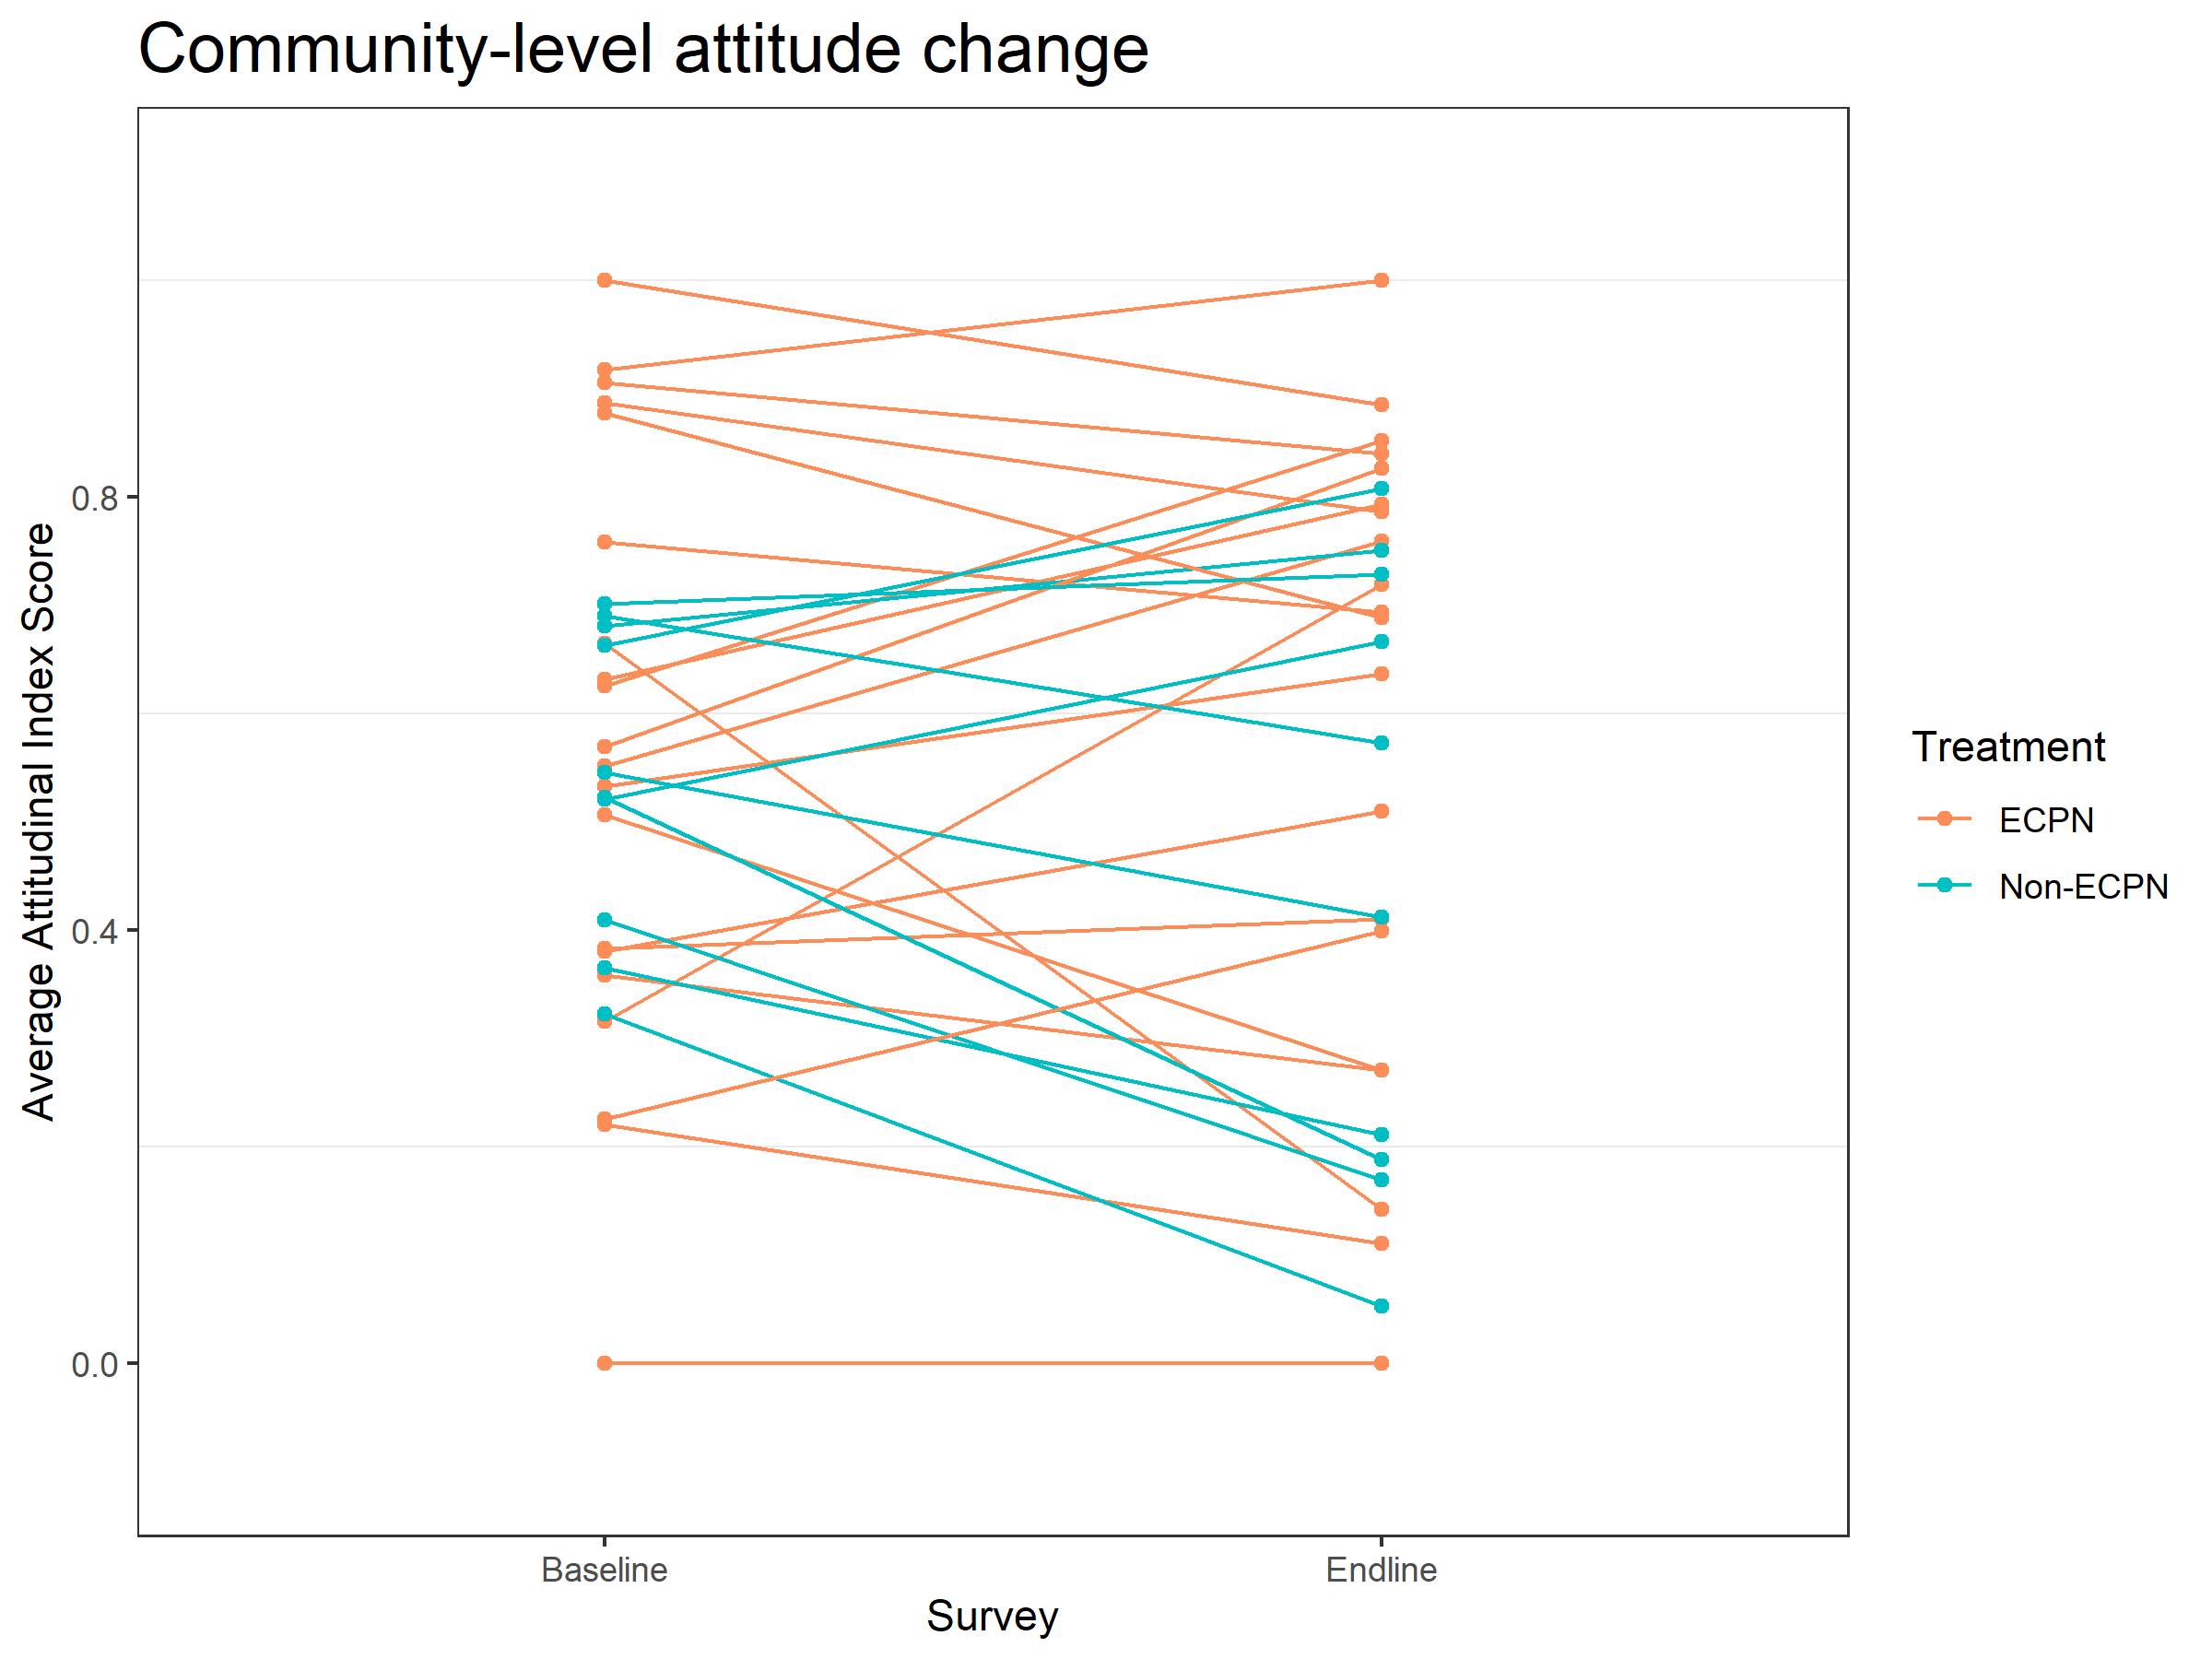
\includegraphics[width=\linewidth]{../survey_dat/figs/did_plots/attitudeComm.plot_disag.png}
\caption{Each point represents a community. This graph shows (1) that overall changes are not driven by a large change in a single community and (2) that the overall change does not reflect a ceiling or floor effect.}\label{fig:att_comm_dis}
\end{figure}

\begin{Shaded}
\begin{Highlighting}[]
\DocumentationTok{\#\# contact}
\FunctionTok{summary}\NormalTok{(ag.df}\SpecialCharTok{$}\NormalTok{contactOnly\_cw[ag.df}\SpecialCharTok{$}\NormalTok{treatment }\SpecialCharTok{\%in\%} \DecValTok{1}\NormalTok{])}
\end{Highlighting}
\end{Shaded}

\begin{verbatim}
##     Min.  1st Qu.   Median     Mean  3rd Qu.     Max. 
## -0.62941 -0.11906  0.03868  0.03011  0.14413  0.57192
\end{verbatim}

\begin{Shaded}
\begin{Highlighting}[]
\FunctionTok{summary}\NormalTok{(ag.df}\SpecialCharTok{$}\NormalTok{contactOnly\_cw[ag.df}\SpecialCharTok{$}\NormalTok{treatment }\SpecialCharTok{\%in\%} \DecValTok{0}\NormalTok{])}
\end{Highlighting}
\end{Shaded}

\begin{verbatim}
##     Min.  1st Qu.   Median     Mean  3rd Qu.     Max. 
## -0.66520 -0.24964 -0.11401 -0.10767  0.08487  0.45330
\end{verbatim}

\begin{figure}%[\sidecaptionrelwidth][t]
\centering
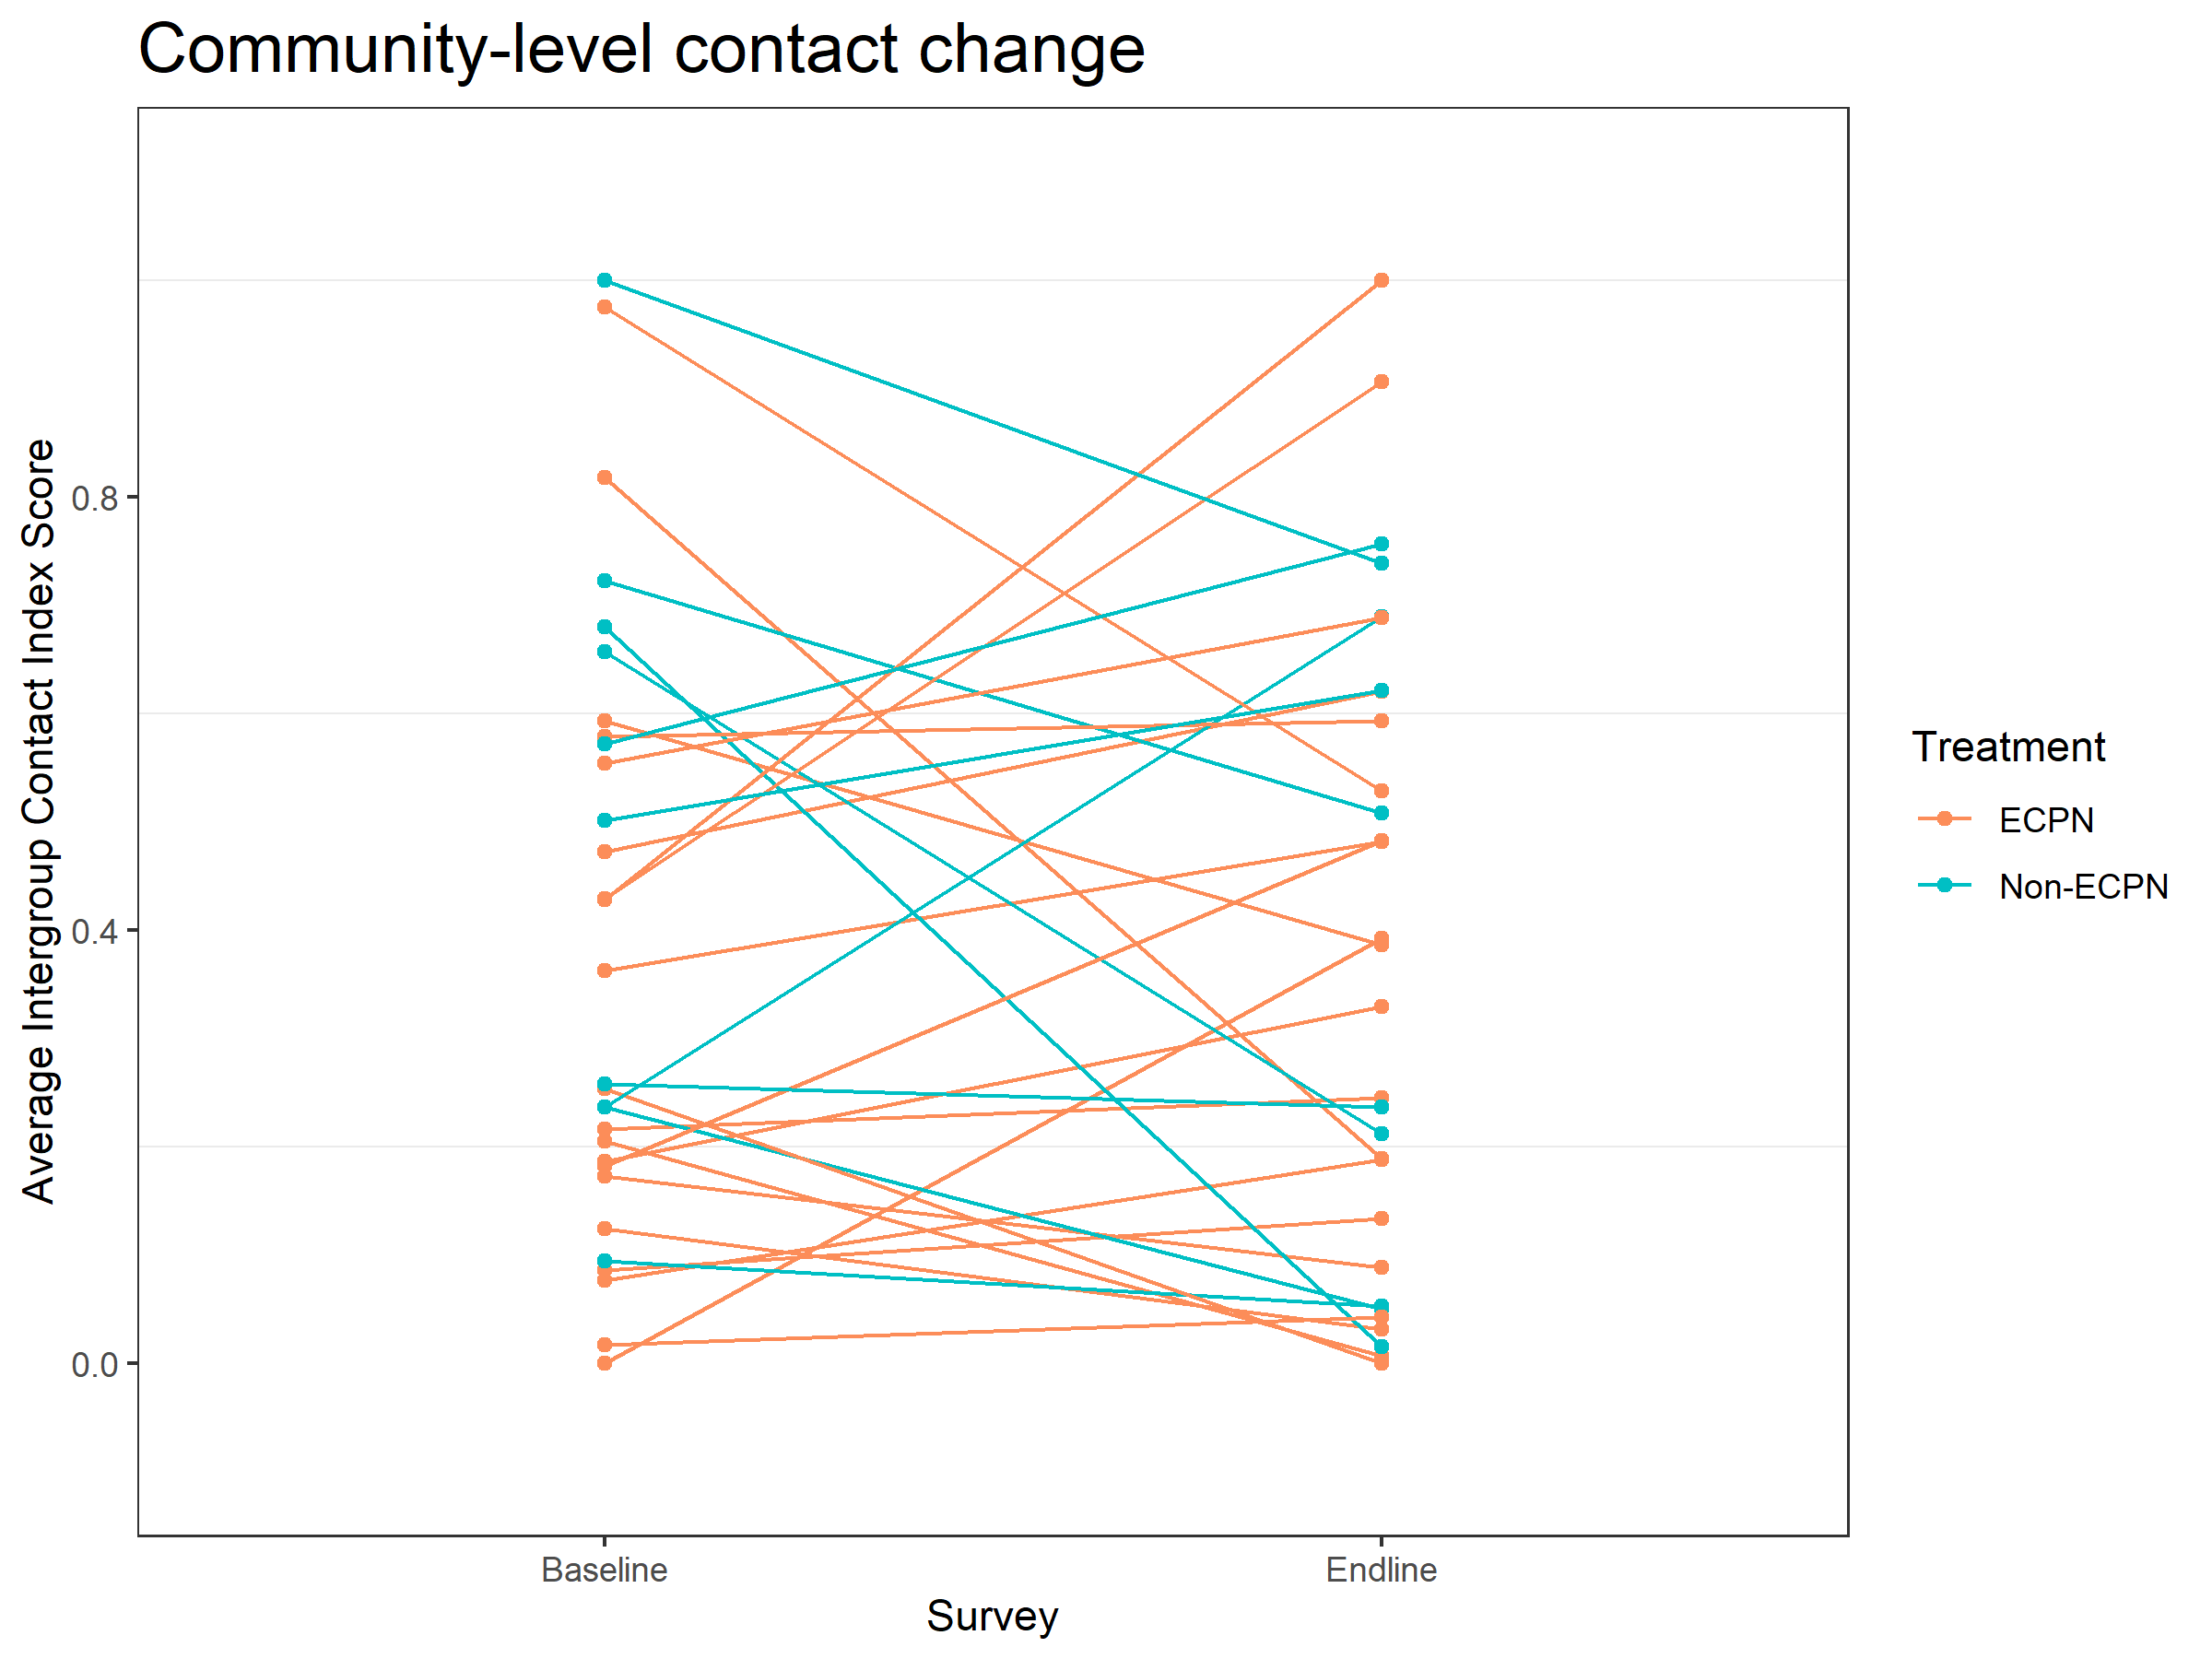
\includegraphics[width=\linewidth]{../survey_dat/figs/did_plots/conComm_plot_disag.png}
\caption{Each point represents a community. This graph shows (1) that overall changes are not driven by a large change in a single community and (2) that the overall change does not reflect a ceiling or floor effect.}\label{fig:con_comm_dis}
\end{figure}

\begin{Shaded}
\begin{Highlighting}[]
\DocumentationTok{\#\# insecurity}
\FunctionTok{summary}\NormalTok{(ag.df}\SpecialCharTok{$}\NormalTok{in\_cw[ag.df}\SpecialCharTok{$}\NormalTok{treatment }\SpecialCharTok{\%in\%} \DecValTok{1}\NormalTok{])}
\end{Highlighting}
\end{Shaded}

\begin{verbatim}
##    Min. 1st Qu.  Median    Mean 3rd Qu.    Max. 
## -0.2871  0.1813  0.2407  0.2143  0.3228  0.4934
\end{verbatim}

\begin{Shaded}
\begin{Highlighting}[]
\FunctionTok{summary}\NormalTok{(ag.df}\SpecialCharTok{$}\NormalTok{in\_cw[ag.df}\SpecialCharTok{$}\NormalTok{treatment }\SpecialCharTok{\%in\%} \DecValTok{0}\NormalTok{])}
\end{Highlighting}
\end{Shaded}

\begin{verbatim}
##     Min.  1st Qu.   Median     Mean  3rd Qu.     Max. 
## -0.17207 -0.08185 -0.04118  0.05516  0.22691  0.41297
\end{verbatim}

\begin{figure}%[\sidecaptionrelwidth][t]
\centering
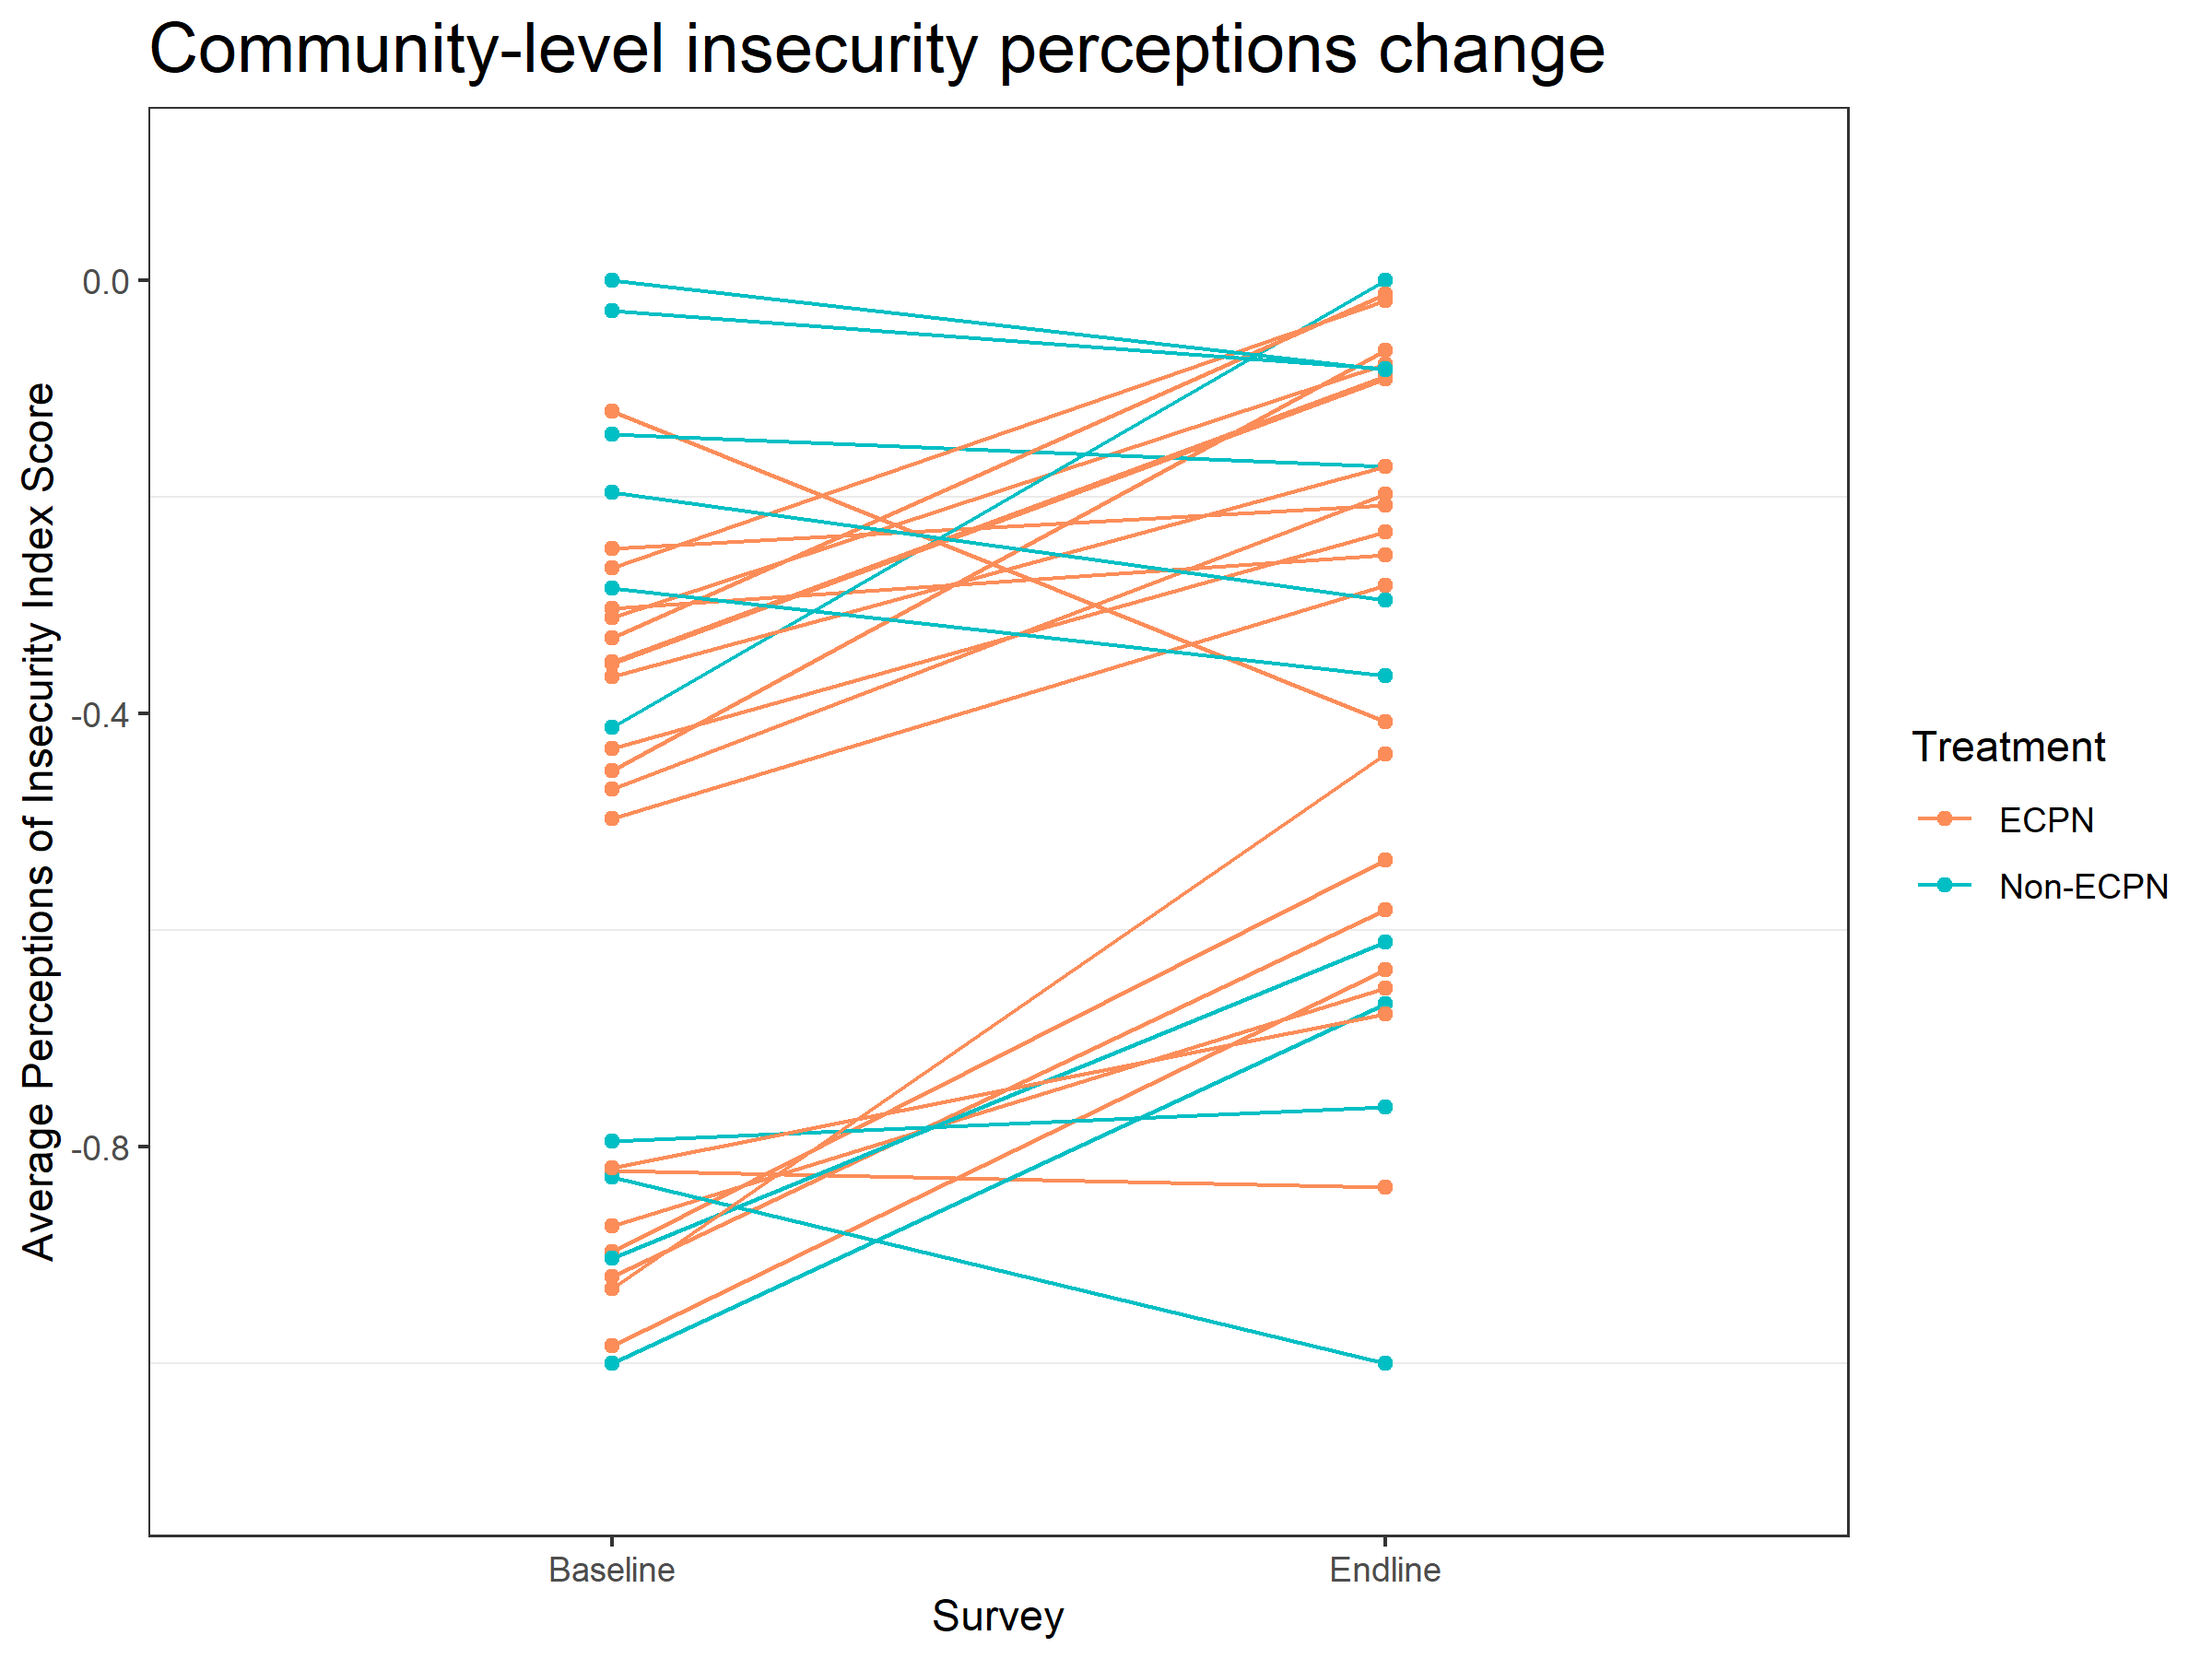
\includegraphics[width=\linewidth]{../survey_dat/figs/did_plots/inComm_plot_disag.png}
\caption{Each point represents a community. This graph shows (1) that overall changes are not driven by a large change in a single community and (2) that the overall change does not reflect a ceiling or floor effect.}\label{fig:in_comm_dis}
\end{figure}

Chris: this section also add all finished DiD plots with lines only for
TR and CO aggregated together, including endorsement exp and percent
exp.

\hypertarget{behavioral-outcomes}{%
\subsubsection{Behavioral outcomes}\label{behavioral-outcomes}}

Skipped summary stats for most of these.

\hypertarget{markets-pastoralist-index}{%
\paragraph{Markets: pastoralist index}\label{markets-pastoralist-index}}

\begin{Shaded}
\begin{Highlighting}[]
\CommentTok{\# Events: pastoralists index}
\FunctionTok{summary}\NormalTok{(events}\SpecialCharTok{$}\NormalTok{pastoralists\_index\_rank[events}\SpecialCharTok{$}\NormalTok{treatment }\SpecialCharTok{\%in\%} \DecValTok{1} \SpecialCharTok{\&}
\NormalTok{                                       events}\SpecialCharTok{$}\NormalTok{time }\SpecialCharTok{\%in\%} \DecValTok{0}\NormalTok{])}
\end{Highlighting}
\end{Shaded}

\begin{verbatim}
##    Min. 1st Qu.  Median    Mean 3rd Qu.    Max. 
##    7.50   16.00   34.00   41.07   66.00   86.00
\end{verbatim}

\begin{Shaded}
\begin{Highlighting}[]
\FunctionTok{summary}\NormalTok{(events}\SpecialCharTok{$}\NormalTok{pastoralists\_index\_rank[events}\SpecialCharTok{$}\NormalTok{treatment }\SpecialCharTok{\%in\%} \DecValTok{1} \SpecialCharTok{\&}
\NormalTok{                                       events}\SpecialCharTok{$}\NormalTok{time }\SpecialCharTok{\%in\%} \DecValTok{1}\NormalTok{])}
\end{Highlighting}
\end{Shaded}

\begin{verbatim}
##    Min. 1st Qu.  Median    Mean 3rd Qu.    Max. 
##    2.50   20.00   36.00   39.48   58.50   84.50
\end{verbatim}

\begin{Shaded}
\begin{Highlighting}[]
\FunctionTok{summary}\NormalTok{(events}\SpecialCharTok{$}\NormalTok{pastoralists\_index\_rank[events}\SpecialCharTok{$}\NormalTok{treatment }\SpecialCharTok{\%in\%} \DecValTok{0} \SpecialCharTok{\&}
\NormalTok{                                       events}\SpecialCharTok{$}\NormalTok{time }\SpecialCharTok{\%in\%} \DecValTok{0}\NormalTok{])}
\end{Highlighting}
\end{Shaded}

\begin{verbatim}
##    Min. 1st Qu.  Median    Mean 3rd Qu.    Max. 
##   22.50   39.50   54.00   59.34   80.50   92.00
\end{verbatim}

\begin{Shaded}
\begin{Highlighting}[]
\FunctionTok{summary}\NormalTok{(events}\SpecialCharTok{$}\NormalTok{pastoralists\_index\_rank[events}\SpecialCharTok{$}\NormalTok{treatment }\SpecialCharTok{\%in\%} \DecValTok{0} \SpecialCharTok{\&}
\NormalTok{                                       events}\SpecialCharTok{$}\NormalTok{time }\SpecialCharTok{\%in\%} \DecValTok{1}\NormalTok{])}
\end{Highlighting}
\end{Shaded}

\begin{verbatim}
##    Min. 1st Qu.  Median    Mean 3rd Qu.    Max. 
##    2.50   23.25   47.00   46.37   68.00   88.00
\end{verbatim}

\begin{figure}%[\sidecaptionrelwidth][t]
\centering
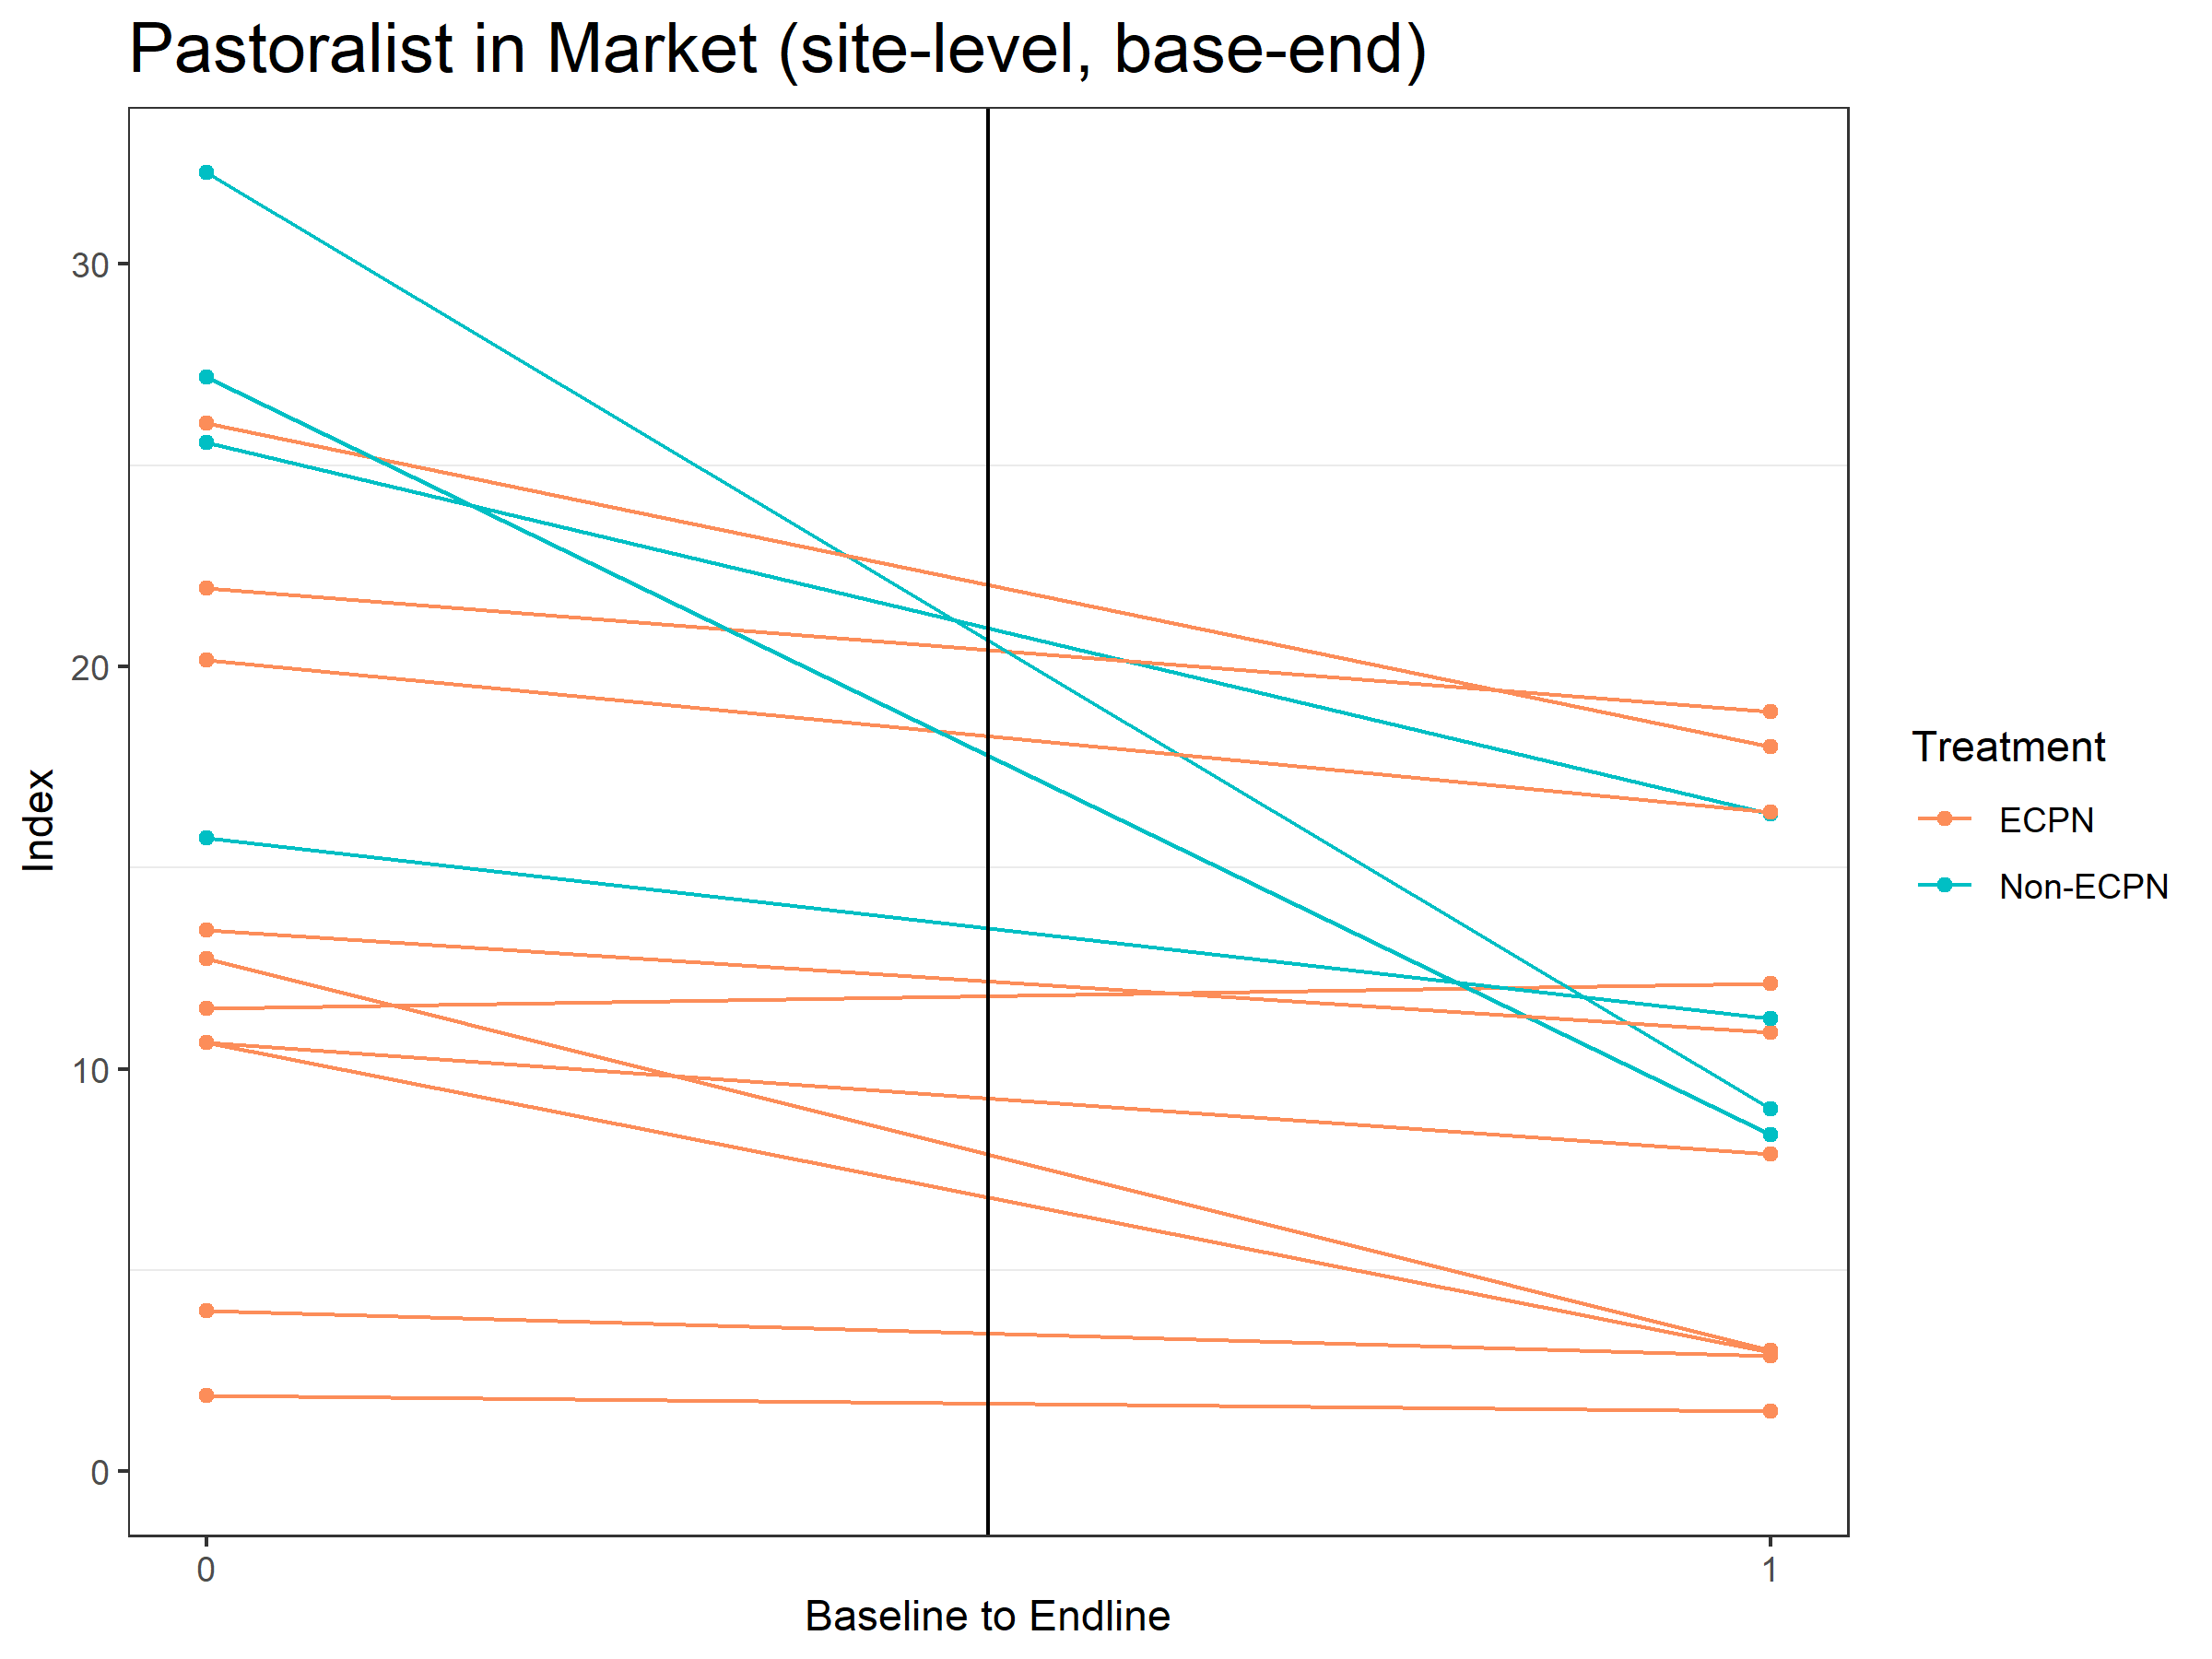
\includegraphics[width=\linewidth]{../obs_dat/b_analysis/market_pasts_siteTime.plot.png}
\caption{Each point represents a site. This graph shows (1) that overall changes are not driven by a large change in a single community and (2) that the overall change does not reflect a ceiling or floor effect.}\label{fig:market_past_siteTime}
\end{figure}

\hypertarget{markets-farmers-index}{%
\paragraph{Markets: farmers index}\label{markets-farmers-index}}

\begin{figure}%[\sidecaptionrelwidth][t]
\centering
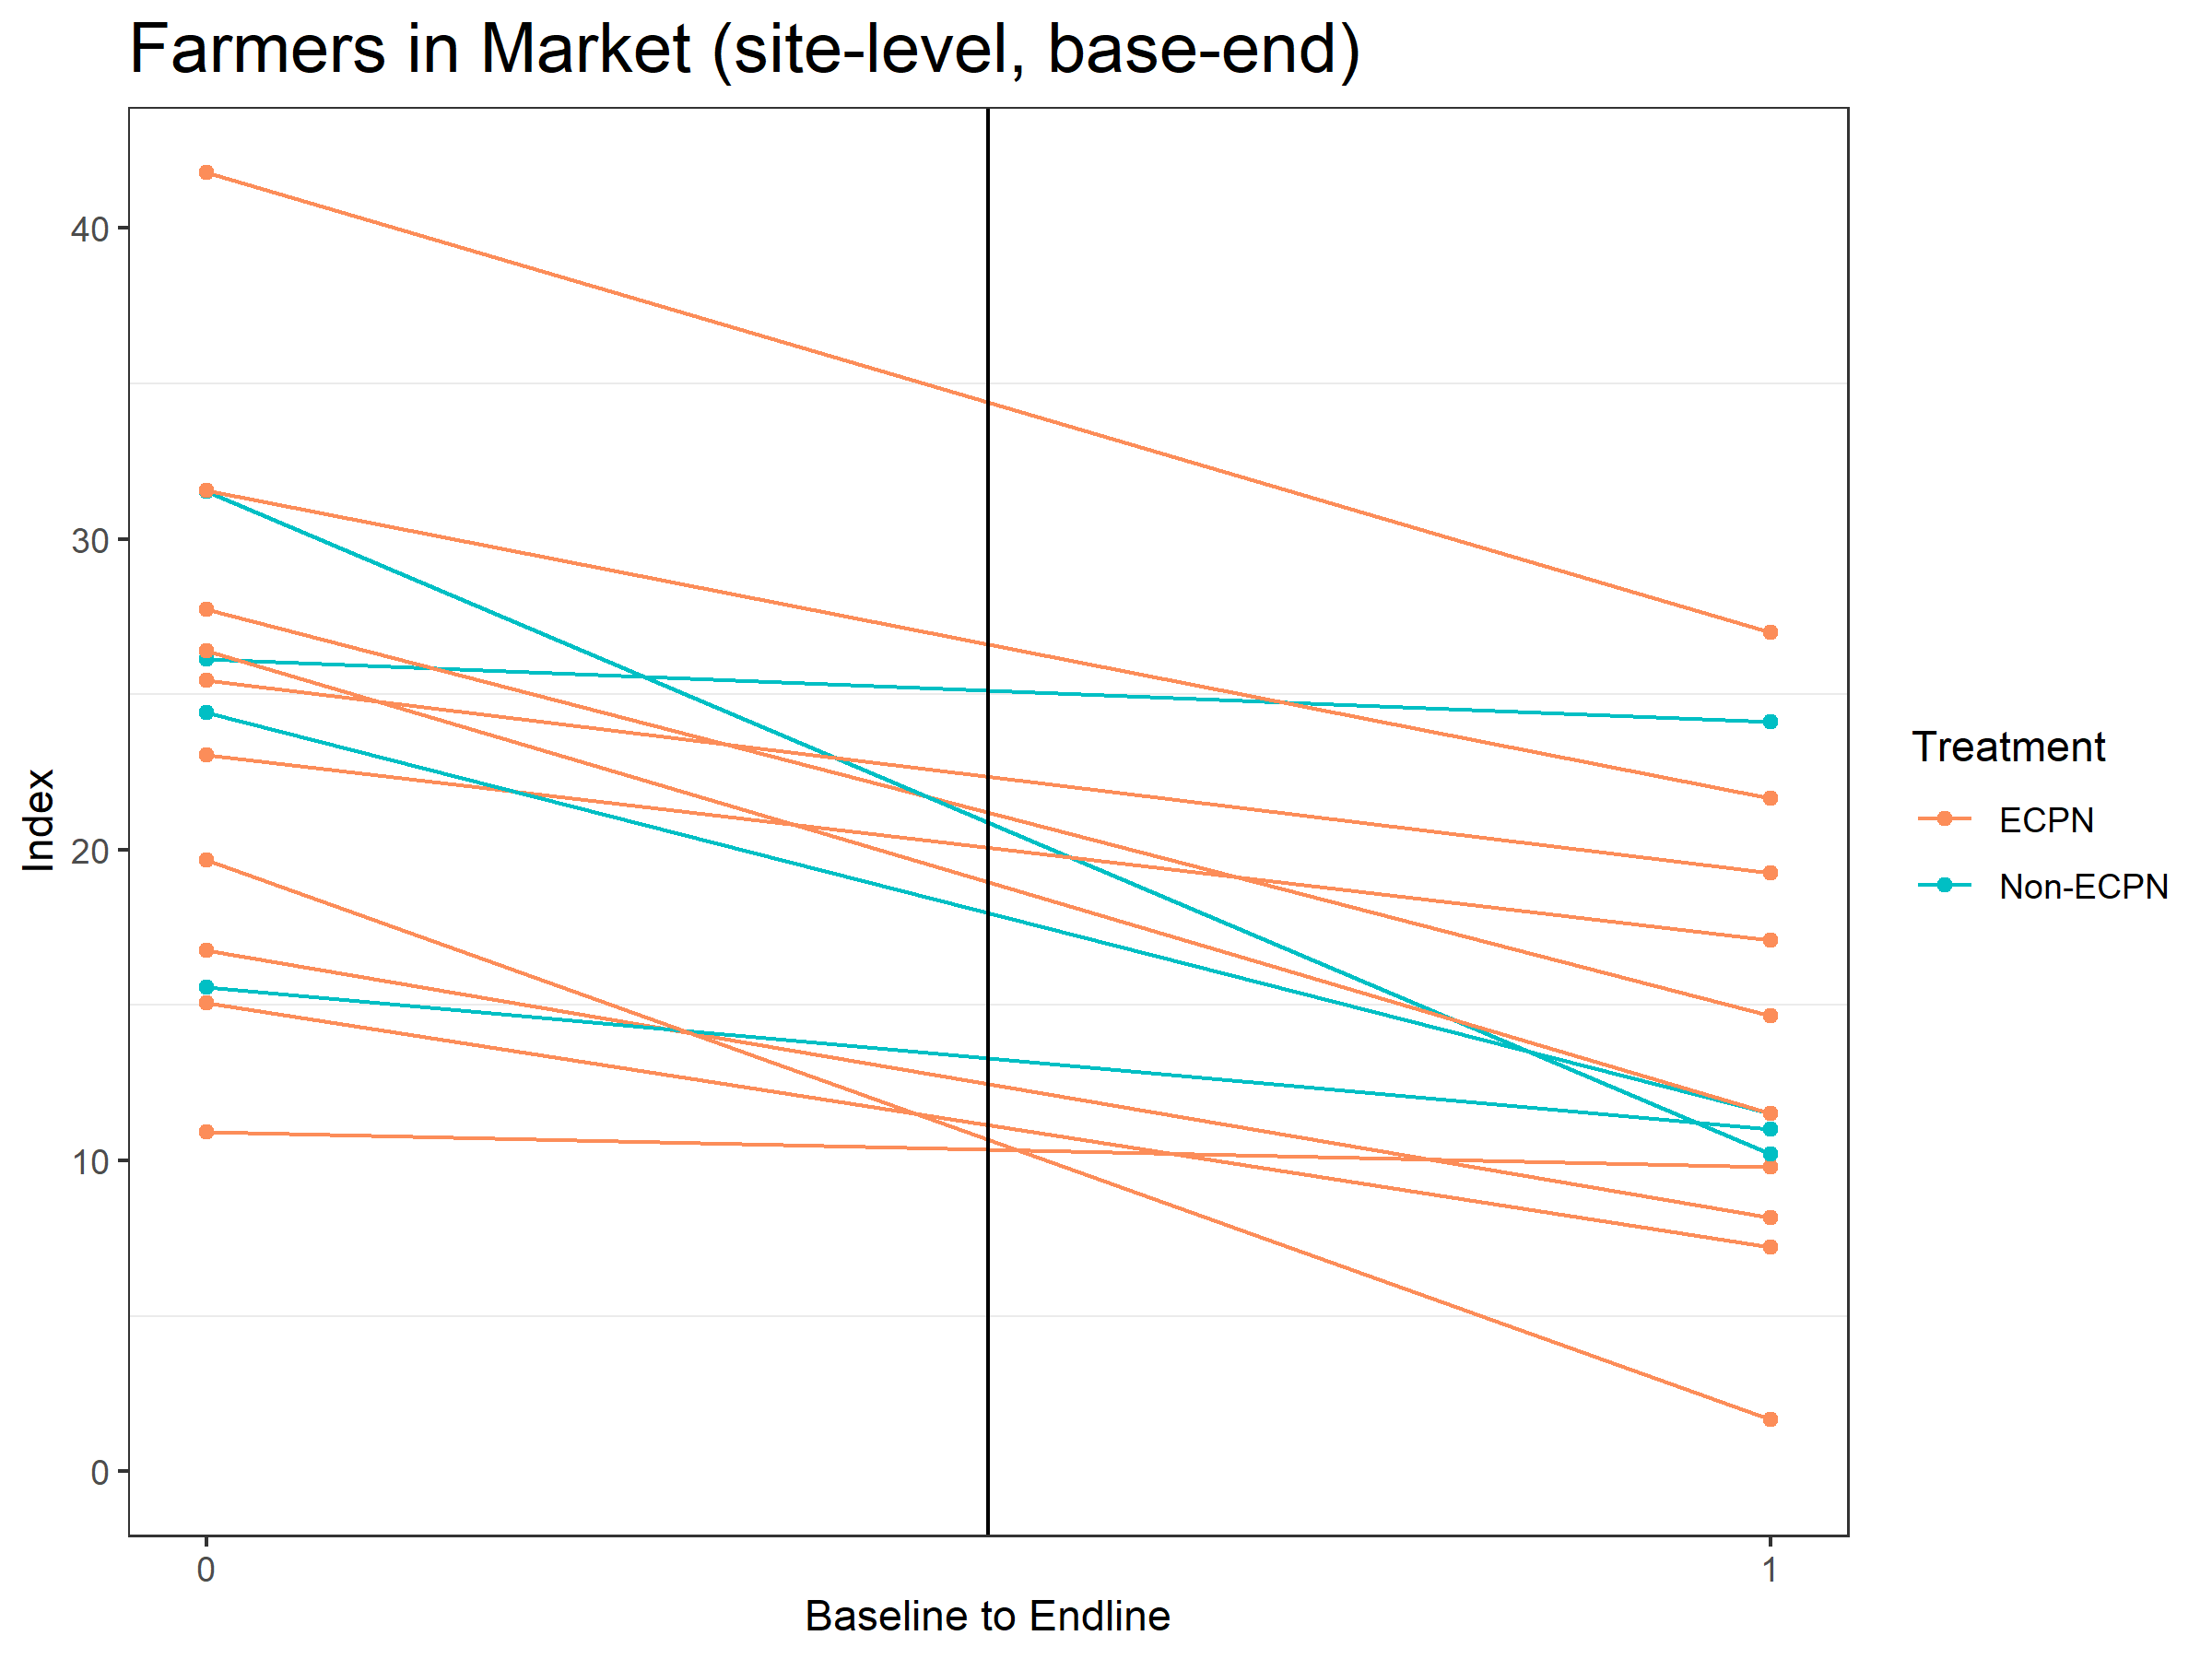
\includegraphics[width=\linewidth]{../obs_dat/b_analysis/market_farms_siteTime.plot.png}
\caption{Each point represents a site. This graph shows (1) that overall changes are not driven by a large change in a single community and (2) that the overall change does not reflect a ceiling or floor effect.}\label{fig:market_farm_siteTime}
\end{figure}

\hypertarget{events-outgroup-index}{%
\paragraph{Events: Outgroup index}\label{events-outgroup-index}}

\begin{figure}%[\sidecaptionrelwidth][t]
\centering
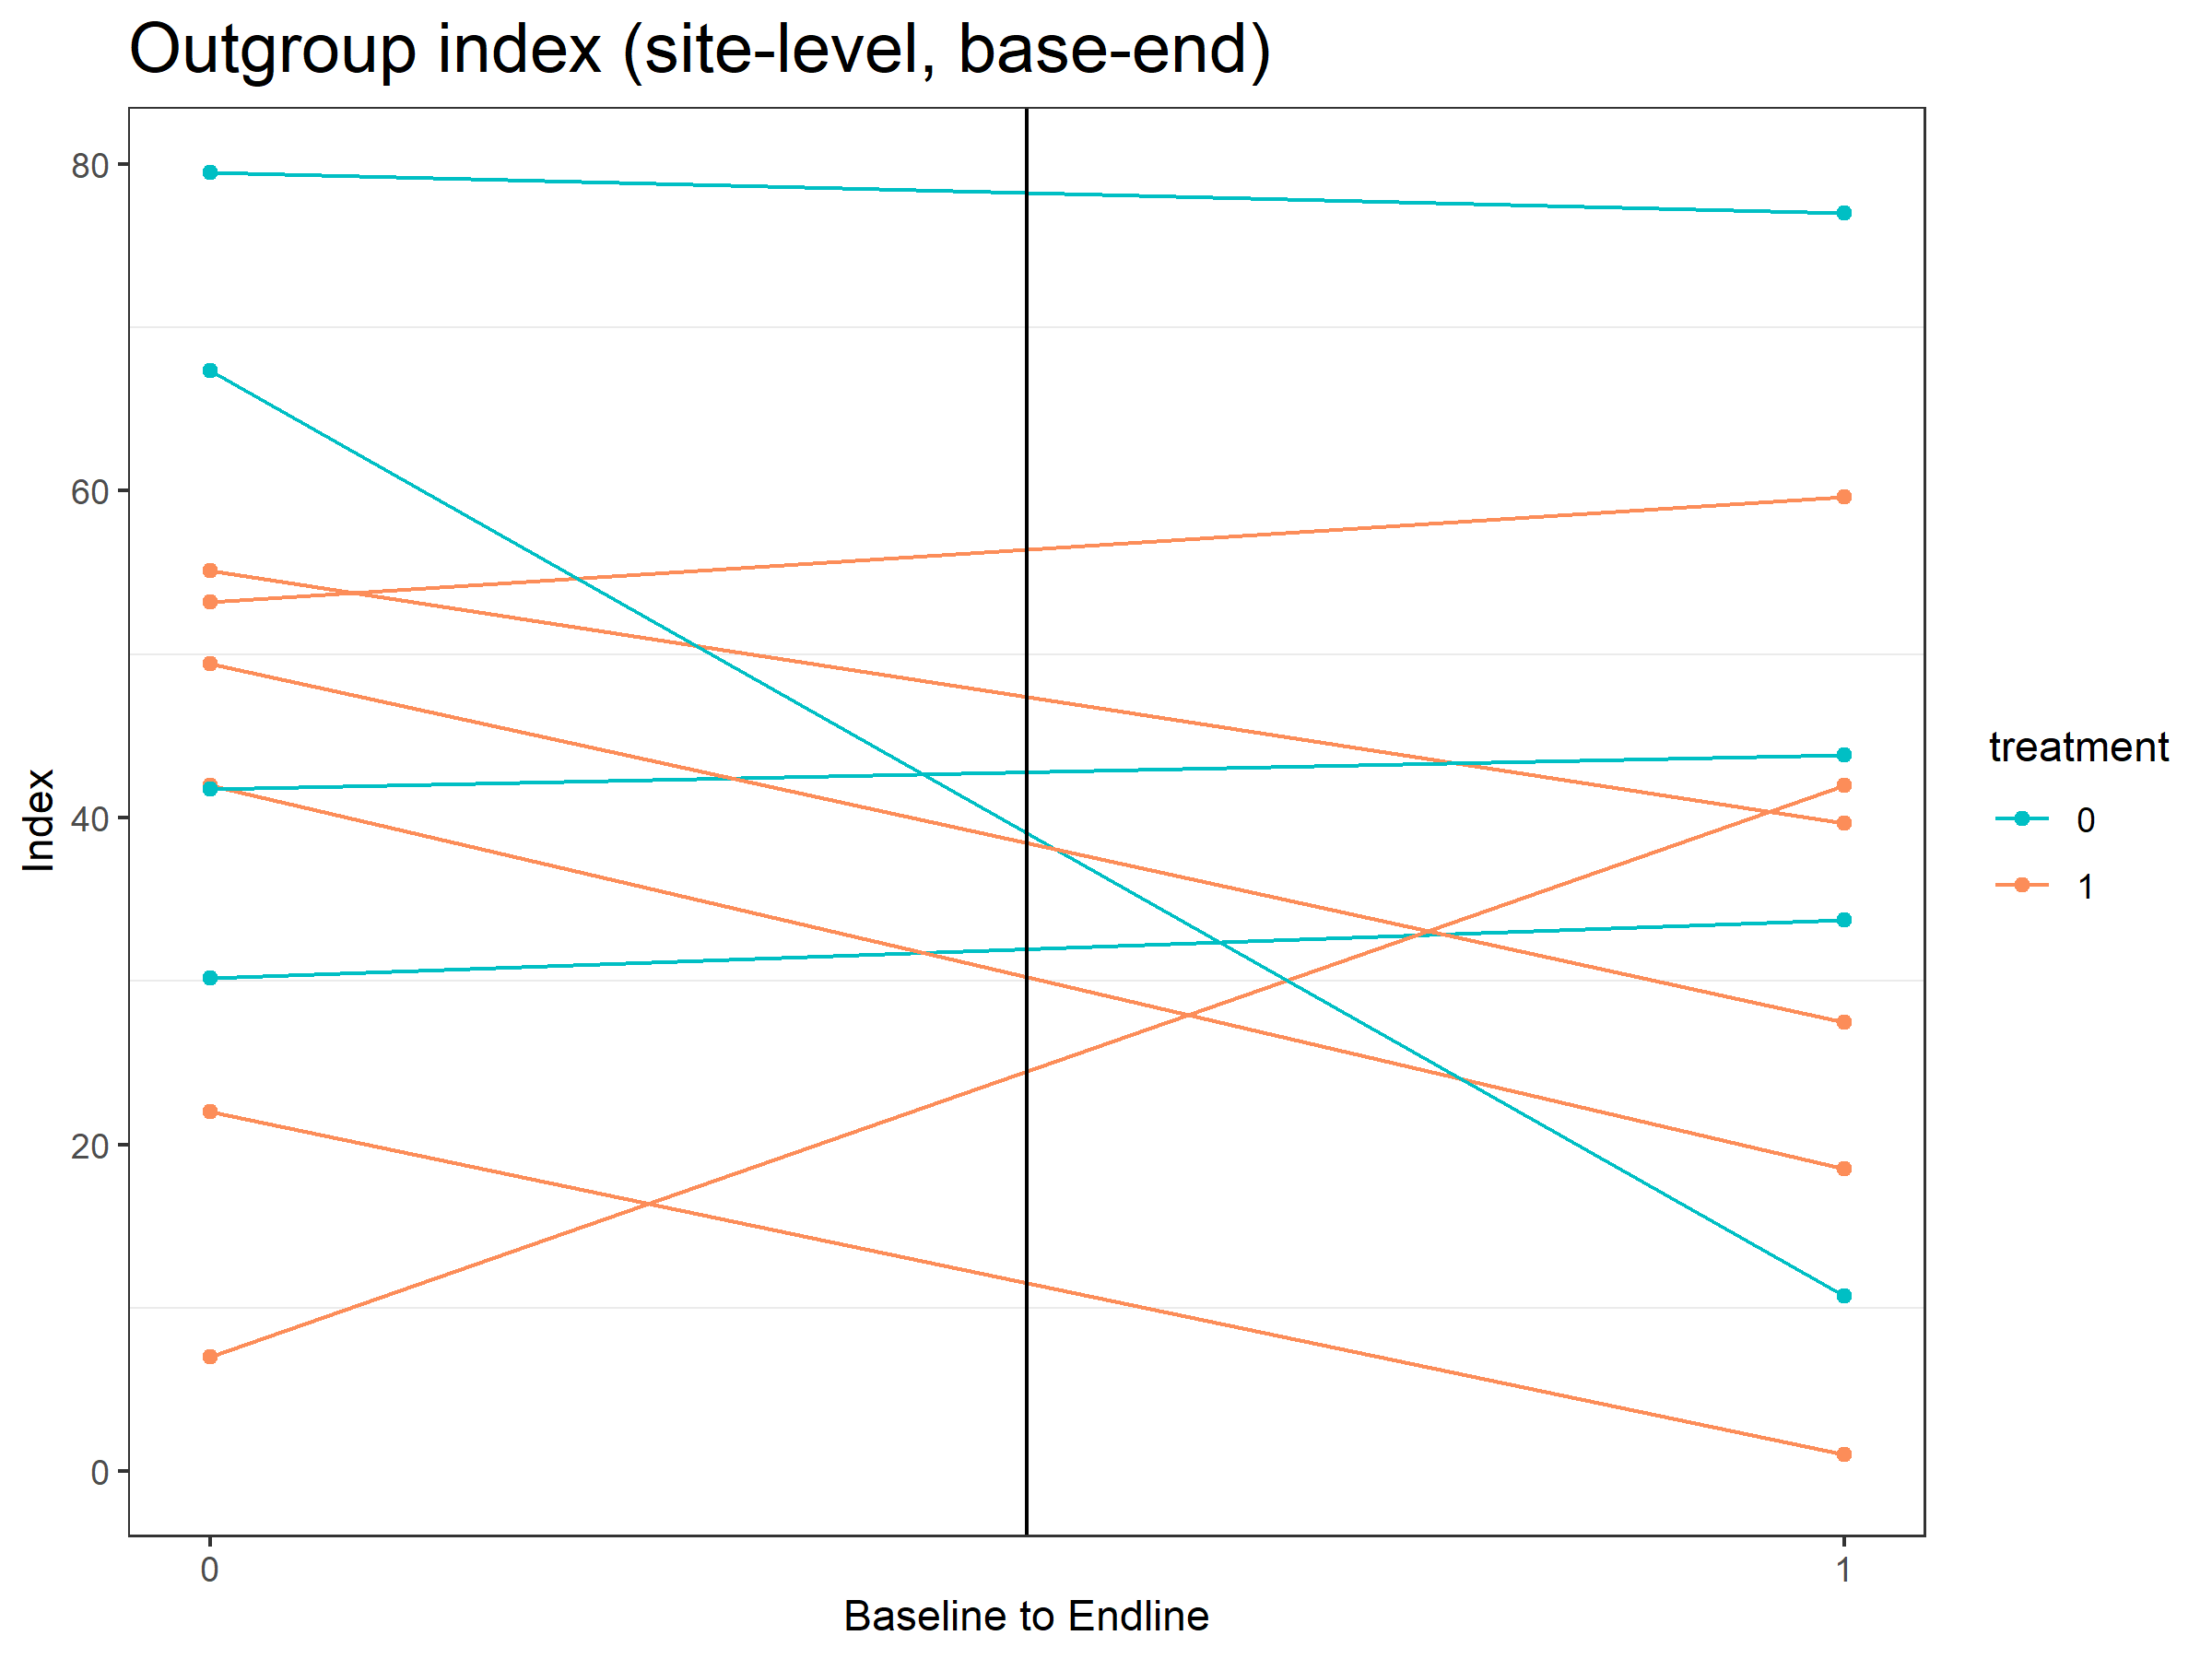
\includegraphics[width=\linewidth]{../obs_dat/b_analysis/events_outgroup_siteTime.plot.png}
\caption{Each point represents a site. This graph shows (1) that overall changes are not driven by a large change in a single community and (2) that the overall change does not reflect a ceiling or floor effect.}\label{fig:events_outgroup_siteTime}
\end{figure}

\hypertarget{comment-5}{%
\subsection{Comment 5}\label{comment-5}}

Lots of the findings are not statistically significant (e.g., Figure 3
seems to show that none of the effects on non-participants were
statistically distinguishable from zero). Sometimes such estimates are
treated as null effects and other times as impacts that are not
statistically significant. It would be helpful to understand how the
authors make such distinctions.

\textbf{Response} Thank you, that is correct that the non-participants
were not statistically different from the control group. We need to be
consistent with wording.

.1 marginal .2 a potential trend /\textgreater.2 null

\begin{Shaded}
\begin{Highlighting}[]
\CommentTok{\# For exact p{-}values: Appendix B for community{-}level analysis, Appendix C for individual{-}level.}
\end{Highlighting}
\end{Shaded}

\hypertarget{comment-6-smaller-questions}{%
\subsection{Comment 6 (smaller
questions)}\label{comment-6-smaller-questions}}

Finally, a few smaller questions: • Why are conflict and violence not
included as dependent variables? There is an assumption that violence is
caused by poor intergroup attitudes, but it is possible that attitudes
could be improved without reducing violence. This seems important both
theoretically and practically.

\textbf{Response} Good question. We have the footnote about it. It's a
good idea but we weren't able to measure that. We have: violence\_effect
``In any clash that occurred in the last year, were you or anyone in
your family negatively affected by an attack caused by {[}X group{]}''

\begin{Shaded}
\begin{Highlighting}[]
\CommentTok{\#violence\_effect}
\FunctionTok{with}\NormalTok{(rand.df[rand.df}\SpecialCharTok{$}\NormalTok{survey }\SpecialCharTok{\%in\%} \DecValTok{0}\NormalTok{,], }\FunctionTok{prop.table}\NormalTok{(}\FunctionTok{table}\NormalTok{(violence\_effect\_num, treatment),}\DecValTok{2}\NormalTok{))}
\end{Highlighting}
\end{Shaded}

\begin{verbatim}
##                    treatment
## violence_effect_num          0          1
##                 0   0.38281250 0.47322298
##                 0.2 0.10351562 0.05842259
##                 0.4 0.14062500 0.08276534
##                 0.6 0.17578125 0.15481986
##                 0.8 0.13085938 0.13047712
##                 1   0.06640625 0.10029211
\end{verbatim}

\begin{Shaded}
\begin{Highlighting}[]
\FunctionTok{with}\NormalTok{(rand.df[rand.df}\SpecialCharTok{$}\NormalTok{survey }\SpecialCharTok{\%in\%} \DecValTok{1}\NormalTok{,], }\FunctionTok{prop.table}\NormalTok{(}\FunctionTok{table}\NormalTok{(violence\_effect\_num, treatment),}\DecValTok{2}\NormalTok{))}
\end{Highlighting}
\end{Shaded}

\begin{verbatim}
##                    treatment
## violence_effect_num          0          1
##                 0   0.77976190 0.76622137
##                 0.2 0.03571429 0.03435115
##                 0.4 0.03174603 0.02958015
##                 0.6 0.04563492 0.04293893
##                 0.8 0.03571429 0.06106870
##                 1   0.07142857 0.06583969
\end{verbatim}

\begin{Shaded}
\begin{Highlighting}[]
\CommentTok{\# violence work effect}
\FunctionTok{with}\NormalTok{(rand.df[rand.df}\SpecialCharTok{$}\NormalTok{survey }\SpecialCharTok{\%in\%} \DecValTok{0}\NormalTok{,], }\FunctionTok{prop.table}\NormalTok{(}\FunctionTok{table}\NormalTok{(violence\_work\_effect, treatment),}\DecValTok{2}\NormalTok{))}
\end{Highlighting}
\end{Shaded}

\begin{verbatim}
##                     treatment
## violence_work_effect          0          1
##                    0 0.05671642 0.02086957
##                    1 0.05074627 0.04173913
##                    2 0.07164179 0.04521739
##                    3 0.21194030 0.26782609
##                    4 0.60895522 0.62434783
\end{verbatim}

\begin{Shaded}
\begin{Highlighting}[]
\FunctionTok{with}\NormalTok{(rand.df[rand.df}\SpecialCharTok{$}\NormalTok{survey }\SpecialCharTok{\%in\%} \DecValTok{1}\NormalTok{,], }\FunctionTok{prop.table}\NormalTok{(}\FunctionTok{table}\NormalTok{(violence\_work\_effect, treatment),}\DecValTok{2}\NormalTok{))}
\end{Highlighting}
\end{Shaded}

\begin{verbatim}
##                     treatment
## violence_work_effect          0          1
##                    0 0.09929078 0.13000000
##                    1 0.09929078 0.05000000
##                    2 0.07092199 0.11333333
##                    3 0.25531915 0.17666667
##                    4 0.47517730 0.53000000
\end{verbatim}

• Were the enumerators who carried out the market observations aware of
a community's treatment status? If such observations were not
treatment-blind, should we be concerned about biased reporting of
intergroup contact?

\textbf{Response} Lisa's email .

Method appendix Unaware of hypotheses Enumerator differences: take out
Israel and Hadiza?

\begin{Shaded}
\begin{Highlighting}[]
\DocumentationTok{\#\#\# robustness checks without hadiza/israel}
\FunctionTok{load}\NormalTok{(}\StringTok{"../obs\_dat/b\_analysis/obsDat\_truePs\_rb.rda"}\NormalTok{)}
\DocumentationTok{\#\#\# robustness checks with only hadiza/israel}
\FunctionTok{load}\NormalTok{(}\StringTok{"../obs\_dat/b\_analysis/obsDat\_truePs\_had.rda"}\NormalTok{)}

\CommentTok{\# without}
\NormalTok{behObs\_enumsCheck }\OtherTok{\textless{}{-}} \FunctionTok{rbind}\NormalTok{(mark\_pasts, mark\_pasts\_rb,}
\NormalTok{                           mark\_farms, mark\_farms\_rb,}
\NormalTok{                           out\_ind, out\_ind\_rb)}
\FunctionTok{colnames}\NormalTok{(behObs\_enumsCheck) }\OtherTok{\textless{}{-}} \FunctionTok{c}\NormalTok{(}\StringTok{"coefficient"}\NormalTok{, }\StringTok{"p{-}value"}\NormalTok{)}
\FunctionTok{rownames}\NormalTok{(behObs\_enumsCheck) }\OtherTok{\textless{}{-}} \FunctionTok{c}\NormalTok{(}\StringTok{"market{-}pastoralists\_all"}\NormalTok{,}
                                 \StringTok{"market{-}pastoralists\_without"}\NormalTok{,}
                                 \StringTok{"market{-}farmers\_all"}\NormalTok{,}
                                 \StringTok{"market{-}farmers\_without"}\NormalTok{,}
                                 \StringTok{"events{-}outgroup\_all"}\NormalTok{,}
                                 \StringTok{"events{-}outgroup\_without"}\NormalTok{)}
\NormalTok{behObs\_enumsCheck }\OtherTok{\textless{}{-}} \FunctionTok{round}\NormalTok{(behObs\_enumsCheck,}\DecValTok{3}\NormalTok{)}
\NormalTok{behObs\_enumsCheck\_tab }\OtherTok{\textless{}{-}}\NormalTok{ knitr}\SpecialCharTok{::}\FunctionTok{kable}\NormalTok{(behObs\_enumsCheck, }\AttributeTok{format=}\StringTok{"latex"}\NormalTok{)}

\CommentTok{\# only them}
\NormalTok{behObs\_enumsOnly }\OtherTok{\textless{}{-}} \FunctionTok{rbind}\NormalTok{(mark\_pasts\_had, mark\_farms\_had, out\_ind\_had)}
\FunctionTok{colnames}\NormalTok{(behObs\_enumsOnly) }\OtherTok{\textless{}{-}} \FunctionTok{c}\NormalTok{(}\StringTok{"coefficient"}\NormalTok{, }\StringTok{"p{-}value"}\NormalTok{)}
\FunctionTok{rownames}\NormalTok{(behObs\_enumsOnly) }\OtherTok{\textless{}{-}} \FunctionTok{c}\NormalTok{(}\StringTok{"market{-}pastoralists\_enum"}\NormalTok{,}
                                 \StringTok{"market{-}farmers\_enum"}\NormalTok{,}
                                 \StringTok{"events{-}outgroup\_enum"}\NormalTok{)}
\NormalTok{behObs\_enumsOnly\_tab }\OtherTok{\textless{}{-}}\NormalTok{ knitr}\SpecialCharTok{::}\FunctionTok{kable}\NormalTok{(behObs\_enumsOnly, }\AttributeTok{format=}\StringTok{"latex"}\NormalTok{)}

\CommentTok{\# Save}
\FunctionTok{save}\NormalTok{(behObs\_enumsCheck\_tab, }\AttributeTok{file=}\StringTok{"behObs\_enumsCheck\_tab.Rda"}\NormalTok{)}
\FunctionTok{save}\NormalTok{(behObs\_enumsOnly\_tab, }\AttributeTok{file=}\StringTok{"behObs\_enumsOnly\_tab.Rda"}\NormalTok{)}
\end{Highlighting}
\end{Shaded}

\textbf{Chris written description for appendix}: Enumerators (for
surveys and for behavioral observation) were not informed of a
community's treatment status, but two of the enumerators for behavioral
observations interacted with the research team frequently and may have
intuited the study's hypotheses. They also only made observations at
treatment sites. If their intuition of program aims affected their
observations (or if their observations became more positive over time
for other reasons), our estimates of the treatment effect could be
inflated.

We checked the change over time in outcomes they reported.
Descriptively, the two senior enumerators observed \emph{less}
interaction in treatment sites over time, suggesting that they were not
influenced by knowledge of the study's hypotheses. As a robustness
check, we then repeated the main analysis but removed observations from
these two enumerators. Coefficients with their data removed are very
similar to coefficients with their data included; \(p\)-values are
higher mainly as a result of fewer observations (and therefore degrees
of freedom).

\begin{table}[H]
\begin{center}
\label{tab:behObs_enumsOnly_tab}
\caption{\textbf{Robustness check for behavioral observations} This table shows the baseline-endline change in outcomes for the two senior enumerators who may have intuited the study's hypotheses. The first column shows coefficients from OLS regression, the second column shows $p$-values. The row names show outcomes (pastoralists in the market, farmers in the market, and outgroup attending events). The two enumerators reported decreases in market outcomes in treatment sites and no change to event outcomes in treatment sites, suggesting that they were not influenced by knowledge of the study's hypotheses.}
\smallskip

\begin{tabular}{l|r|r}
\hline
  & coefficient & p-value\\
\hline
market-pastoralists\_enum & -4.4079254 & 0.1744306\\
\hline
market-farmers\_enum & -10.8863636 & 0.0161117\\
\hline
events-outgroup\_enum & 0.1363636 & 0.9929502\\
\hline
\end{tabular}


\end{center}
\end{table}

\begin{table}[H]
\begin{center}
\label{tab:behObs_enumsCheck_tab}
\caption{\textbf{Robustness check for behavioral observations} This table shows behavioral observation outcomes with two senior enumerators removed. The first column shows coefficients from OLS regression, the second column shows $p$-values. The row names show outcomes (pastoralists in the market, farmers in the market, and outgroup attending events) and subsets of the data (all data, data without two enumerators, and data from only those two enumerators).}
\smallskip

\begin{tabular}{l|r|r}
\hline
  & coefficient & p-value\\
\hline
market-pastoralists\_all & 12.532 & 0.001\\
\hline
market-pastoralists\_without & 10.285 & 0.103\\
\hline
market-farmers\_all & 3.339 & 0.242\\
\hline
market-farmers\_without & 1.286 & 0.456\\
\hline
events-outgroup\_all & 9.228 & 0.186\\
\hline
events-outgroup\_without & 6.333 & 0.136\\
\hline
\end{tabular}


\end{center}
\end{table}

\hypertarget{review-2}{%
\section{Review 2}\label{review-2}}

\hypertarget{comment-1-1}{%
\subsection{Comment 1}\label{comment-1-1}}

The baseline for our understanding of pastoralist-farmer relations here
refers to conflict. As the authors note circa line 147, relations had
involved positive interactions that arose endogenously (see 167-68). The
intervention here, as well as some of the drivers of contemporary
conflict (ie, climate change) are largely exogenous. This could
interfere with certain aspects of the research design, discussed below.
But I believe it could be sufficiently, appropriately addressed within
the framing of the paper around intergroup theory. For example, Allport
was exploring prejudice and misinformed views about outgroups. Farmers
and pastoralists have different interests, meaning that the attitudes
shaping their interactions are not simply about a lack of information
(or experience with) the other. The authors explore this around line
163. The PGG generates a shared interest, and in his regard the failure,
or limited evidence of cooperation there, is an important limitation of
this study, as the authors concede. I would appreciate a stronger
justification, perhaps within the background about Nigeria itself, for
how the inorganic and engineered contact does not interfere with the
theorized drivers of outcomes. This seems especially important since
participants were provided with mediation training; this made me wonder
if I am observing effects and positive spillover of mediation training
or random social contact that generates ``authentic'' attitudes and
behaviors. Is the contact or the efficacy of the mediation driving
change here?

\textbf{Response} Many good points being made here. We will address each
of them.

Emphasize conditions need to be met. Why intervention was explicitly
designed to meet those conditions. Just encountering can have negative
effects (Enos) We can't disqualify that some of the spillover
contact--for example in the markets--did not also contribute to
outcomes. But that is part of the hope of contact interventions is that
it leads to positive contact outside of the intervention. This is a rare
study that we look at both in the intervention and outside (Mousa an
exception).

Mediation being driving, see response above Lack of information--contact
may apply in both when people have negative attitudes--extensions of
contact theory to situations where knowledge may not be an issues but
still negative beliefs

So in my rereading of the comment, it seems more about that in addition
to lack of knowledge there are differing interests in this situation. So
it's not just about knowledge--there is real resource scarcity. While
the resource scarcity is real, a) it's a common interest to manage it
well and b) there is a history of cooperation. Maybe Kertzer on contact
not improving attitudes if other side wants bad things for you Maybe
other stuff

Maybe concerned with: - artificiality of intervention? - real effect
caused by random social contact that our intervention generated.
Voluntary contact outside of the program is an intended outcome of the
intervention. - these groups have differing interests, intervention
trying to build on common interests. vs most contact interventions:
cause of prejudice/conflict lack of knowledge. Here groups are competing
with one another. Response Empirical question we are answering. beyond
minimal groups, unrealistic that groups have no information. contact can
do more than knowledge -- can change perceptions about degree to which
interests are aligned/misaligned. pettigrew \& tropp meta-analysis about
more than information.

Possible response solution: note that the reviewer makes good points and
this is a complex issue. Then go over the several things we think
reviewer is pointing out, responding to each point.

\hypertarget{comment-2-1}{%
\subsection{Comment 2}\label{comment-2-1}}

With regard to research design, I would appreciate a stronger
justification of the site selection. As the authors note, Benue has
embraced especially strong policies biased against pastoralists (it was
one of the first states to ban ``open grazing''). The intervention is
therefore correcting for a manufactured imbalance between the groups, in
a way: pastoralists likely feel insecure when the state sided with
farmers and organized militias on their behalf. This is also a condition
that is arguably different from Nasarawa. Perhaps this is adequately
captured in the fixed effects models noted in the supplemental info.
Secondly, the description of the group identities is standard,
characterizing pastoralists as overwhelmingly Fulani and Muslim etc.
There might be little reason to question this, but I noticed that
individual characteristics are dropped from the survey analysis in the
supplemental index\ldots if I am understanding that reference properly.

\textbf{Response} In appendix: - table showing demographic
characteristics of fulani vs farmers: (1) overall, (2) benue, (3)
nasarawa - add exploratory regression that also uses individual's
demographic characteristics? Potentially add something about site
selection or clarify the anti-grazing policies were implemented after
site selection.

\begin{Shaded}
\begin{Highlighting}[]
\CommentTok{\# table showing demographic characteristics of fulani vs farmers: (1) overall, (2) benue, (3) nasarawa}
\DocumentationTok{\#\# make variables}
\NormalTok{rand.df}\SpecialCharTok{$}\NormalTok{survey }\OtherTok{\textless{}{-}} \FunctionTok{ifelse}\NormalTok{(rand.df}\SpecialCharTok{$}\NormalTok{survey }\SpecialCharTok{\%in\%} \DecValTok{0}\NormalTok{, }\StringTok{"baseline"}\NormalTok{, }\StringTok{"endline"}\NormalTok{)}
\NormalTok{rand.df}\SpecialCharTok{$}\NormalTok{christian }\OtherTok{\textless{}{-}} \FunctionTok{ifelse}\NormalTok{(rand.df}\SpecialCharTok{$}\NormalTok{religion }\SpecialCharTok{\%in\%} \StringTok{"christian"}\NormalTok{, }\DecValTok{1}\NormalTok{, }\DecValTok{0}\NormalTok{)}
\NormalTok{rand.df}\SpecialCharTok{$}\NormalTok{muslim }\OtherTok{\textless{}{-}} \FunctionTok{ifelse}\NormalTok{(rand.df}\SpecialCharTok{$}\NormalTok{religion }\SpecialCharTok{\%in\%} \StringTok{"muslim"}\NormalTok{, }\DecValTok{1}\NormalTok{, }\DecValTok{0}\NormalTok{)}
\NormalTok{rand.df}\SpecialCharTok{$}\NormalTok{farming }\OtherTok{\textless{}{-}} \FunctionTok{ifelse}\NormalTok{(rand.df}\SpecialCharTok{$}\NormalTok{occupation }\SpecialCharTok{\%in\%} \FunctionTok{c}\NormalTok{(}\StringTok{"farm"}\NormalTok{,}\StringTok{"both"}\NormalTok{), }\DecValTok{1}\NormalTok{, }\DecValTok{0}\NormalTok{)}
\NormalTok{rand.df}\SpecialCharTok{$}\NormalTok{pastoral }\OtherTok{\textless{}{-}} \FunctionTok{ifelse}\NormalTok{(rand.df}\SpecialCharTok{$}\NormalTok{occupation }\SpecialCharTok{\%in\%} \FunctionTok{c}\NormalTok{(}\StringTok{"pastor"}\NormalTok{,}\StringTok{"both"}\NormalTok{), }\DecValTok{1}\NormalTok{, }\DecValTok{0}\NormalTok{)}
\NormalTok{rand.df}\SpecialCharTok{$}\NormalTok{trading }\OtherTok{\textless{}{-}} \FunctionTok{ifelse}\NormalTok{(rand.df}\SpecialCharTok{$}\NormalTok{occupation }\SpecialCharTok{\%in\%} \StringTok{"trade"}\NormalTok{, }\DecValTok{1}\NormalTok{, }\DecValTok{0}\NormalTok{)}
\NormalTok{rand.df}\SpecialCharTok{$}\NormalTok{fulani }\OtherTok{\textless{}{-}}\NormalTok{ rand.df}\SpecialCharTok{$}\NormalTok{ethnic2fulani}
\NormalTok{rand.df}\SpecialCharTok{$}\NormalTok{income }\OtherTok{\textless{}{-}}\NormalTok{ rand.df}\SpecialCharTok{$}\NormalTok{income\_month}

\DocumentationTok{\#\# List of group variables and summary variables}
\NormalTok{group\_vars }\OtherTok{\textless{}{-}} \FunctionTok{c}\NormalTok{(}\StringTok{"farm\_pastor"}\NormalTok{, }\StringTok{"state"}\NormalTok{, }\StringTok{"survey"}\NormalTok{)}
\NormalTok{summary\_vars }\OtherTok{\textless{}{-}} \FunctionTok{c}\NormalTok{(}\StringTok{"age"}\NormalTok{, }\StringTok{"female"}\NormalTok{, }\StringTok{"income"}\NormalTok{, }
                  \StringTok{"fulani"}\NormalTok{, }\StringTok{"christian"}\NormalTok{, }\StringTok{"muslim"}\NormalTok{,}
                  \StringTok{"farming"}\NormalTok{, }\StringTok{"pastoral"}\NormalTok{, }\StringTok{"trading"}\NormalTok{,}
                  \StringTok{"radio"}\NormalTok{)}

\CommentTok{\#show: age, gender, income, house\_size, ethnic, religion, occupation, radio}
\CommentTok{\# overall}
\NormalTok{demo\_tab\_overall }\OtherTok{\textless{}{-}}\NormalTok{ rand.df }\SpecialCharTok{\%\textgreater{}\%}\NormalTok{ dplyr}\SpecialCharTok{::}\FunctionTok{select}\NormalTok{(farm\_pastor,summary\_vars) }\SpecialCharTok{\%\textgreater{}\%}
  \FunctionTok{group\_by}\NormalTok{(farm\_pastor) }\SpecialCharTok{\%\textgreater{}\%}
  \FunctionTok{summarise}\NormalTok{(}\FunctionTok{across}\NormalTok{(}\FunctionTok{everything}\NormalTok{(), mean, }\AttributeTok{na.rm=}\NormalTok{T))}
\NormalTok{demo\_tab\_overall }\OtherTok{\textless{}{-}} \FunctionTok{cbind}\NormalTok{(demo\_tab\_overall[,}\DecValTok{1}\NormalTok{], }\FunctionTok{round}\NormalTok{(demo\_tab\_overall[,}\DecValTok{2}\SpecialCharTok{:}\FunctionTok{ncol}\NormalTok{(demo\_tab\_overall)],}\DecValTok{2}\NormalTok{))}

\CommentTok{\# by state}
\NormalTok{demo\_tab\_state }\OtherTok{\textless{}{-}}\NormalTok{ rand.df }\SpecialCharTok{\%\textgreater{}\%}\NormalTok{ dplyr}\SpecialCharTok{::}\FunctionTok{select}\NormalTok{(farm\_pastor, state,summary\_vars) }\SpecialCharTok{\%\textgreater{}\%}
  \FunctionTok{group\_by}\NormalTok{(farm\_pastor, state) }\SpecialCharTok{\%\textgreater{}\%}
  \FunctionTok{summarise}\NormalTok{(}\FunctionTok{across}\NormalTok{(}\FunctionTok{everything}\NormalTok{(), mean, }\AttributeTok{na.rm=}\NormalTok{T))}
\end{Highlighting}
\end{Shaded}

\begin{verbatim}
## `summarise()` has grouped output by 'farm_pastor'. You can override using the
## `.groups` argument.
\end{verbatim}

\begin{Shaded}
\begin{Highlighting}[]
\NormalTok{demo\_tab\_state }\OtherTok{\textless{}{-}} \FunctionTok{cbind}\NormalTok{(demo\_tab\_state[,}\DecValTok{1}\SpecialCharTok{:}\DecValTok{2}\NormalTok{], }\FunctionTok{round}\NormalTok{(demo\_tab\_state[,}\DecValTok{3}\SpecialCharTok{:}\FunctionTok{ncol}\NormalTok{(demo\_tab\_state)],}\DecValTok{2}\NormalTok{))}

\CommentTok{\# farm\_pastor,state, survey {-}{-} too complex}
\CommentTok{\#rand.df \%\textgreater{}\% dplyr::select(group\_vars,summary\_vars) \%\textgreater{}\%}
\CommentTok{\#  group\_by(farm\_pastor, survey, state) \%\textgreater{}\%}
\CommentTok{\#  summarise(across(everything(), mean, na.rm=T))}

\CommentTok{\# tables}
\NormalTok{demo\_tab\_overall1 }\OtherTok{\textless{}{-}}\NormalTok{ knitr}\SpecialCharTok{::}\FunctionTok{kable}\NormalTok{(demo\_tab\_overall, }\AttributeTok{format=}\StringTok{"latex"}\NormalTok{)}
\NormalTok{demo\_tab\_state1 }\OtherTok{\textless{}{-}}\NormalTok{ knitr}\SpecialCharTok{::}\FunctionTok{kable}\NormalTok{(demo\_tab\_state, }\AttributeTok{format=}\StringTok{"latex"}\NormalTok{)}

\CommentTok{\# Save}
\FunctionTok{save}\NormalTok{(demo\_tab\_overall1, }\AttributeTok{file=}\StringTok{"demo\_tab\_overall1.Rda"}\NormalTok{)}
\FunctionTok{save}\NormalTok{(demo\_tab\_state1, }\AttributeTok{file=}\StringTok{"demo\_tab\_state1.Rda"}\NormalTok{)}
\end{Highlighting}
\end{Shaded}

\begin{table}[H]
\begin{center}
\label{tab:demo_tab_overall1}
\caption{\textbf{Farmer and Pastoralist Demographics} This table shows demographic characteristics for farming groups and pastoralist groups}
\smallskip

\begin{tabular}{l|r|r|r|r|r|r|r|r|r|r}
\hline
farm\_pastor & age & female & income & fulani & christian & muslim & farming & pastoral & trading & radio\\
\hline
farmers & 36.31 & 0.43 & 42235.09 & 0 & 0.64 & 0.35 & 0.80 & 0.00 & 0.12 & 2.32\\
\hline
pastoralists & 34.66 & 0.46 & 30407.69 & 1 & 0.00 & 1.00 & 0.13 & 0.85 & 0.09 & 1.46\\
\hline
\end{tabular}


\end{center}
\end{table}

\begin{table}[H]
\begin{center}
\label{tab:demo_tab_state1}
\caption{\textbf{Farmer and Pastoralist Demographics by State} This table shows demographic characteristics for farming groups and pastoralist groups, separating respondents from Nasarawa and Benue}
\smallskip

\begin{tabular}{l|l|r|r|r|r|r|r|r|r|r|r}
\hline
farm\_pastor & state & age & female & income & fulani & christian & muslim & farming & pastoral & trading & radio\\
\hline
farmers & ben & 36.32 & 0.41 & 32521.10 & 0 & 0.98 & 0.00 & 0.97 & 0.00 & 0.02 & 2.50\\
\hline
farmers & nas & 36.30 & 0.44 & 48373.50 & 0 & 0.42 & 0.57 & 0.70 & 0.00 & 0.19 & 2.20\\
\hline
pastoralists & ben & 35.04 & 0.39 & 24947.04 & 1 & 0.00 & 1.00 & 0.04 & 0.88 & 0.10 & 1.55\\
\hline
pastoralists & nas & 34.40 & 0.51 & 34050.07 & 1 & 0.00 & 1.00 & 0.18 & 0.83 & 0.08 & 1.40\\
\hline
\end{tabular}


\end{center}
\end{table}

\textbf{add exploratory regression that also uses individual's
demographic characteristics for ag.df}

\begin{Shaded}
\begin{Highlighting}[]
\CommentTok{\#compare to newList coefs}
\NormalTok{compCoefs }\OtherTok{\textless{}{-}} \FunctionTok{sapply}\NormalTok{(newList, }\ControlFlowTok{function}\NormalTok{(x) x}\SpecialCharTok{$}\NormalTok{coef[x}\SpecialCharTok{$}\NormalTok{base }\SpecialCharTok{\%in\%} \DecValTok{1}\NormalTok{])}
\FunctionTok{names}\NormalTok{(compCoefs) }\OtherTok{\textless{}{-}}\NormalTok{ outcome\_list}

\CommentTok{\# make vars for ag.df that aren\textquotesingle{}t in ag.df}
\NormalTok{needVars }\OtherTok{\textless{}{-}} \FunctionTok{c}\NormalTok{(}\StringTok{"christian"}\NormalTok{, }\StringTok{"farming"}\NormalTok{, }\StringTok{"pastoral"}\NormalTok{, }\StringTok{"trading"}\NormalTok{,}
              \StringTok{"income"}\NormalTok{, }\StringTok{"community"}\NormalTok{, }\StringTok{"survey"}\NormalTok{)}
\NormalTok{demo\_df }\OtherTok{\textless{}{-}}\NormalTok{ rand.df }\SpecialCharTok{\%\textgreater{}\%} \FunctionTok{filter}\NormalTok{(survey}\SpecialCharTok{==}\StringTok{"baseline"}\NormalTok{)}\SpecialCharTok{\%\textgreater{}\%}
\NormalTok{  dplyr}\SpecialCharTok{::}\FunctionTok{select}\NormalTok{(}\FunctionTok{all\_of}\NormalTok{(needVars)) }\SpecialCharTok{\%\textgreater{}\%}
  \FunctionTok{group\_by}\NormalTok{(community) }\SpecialCharTok{\%\textgreater{}\%}
  \FunctionTok{summarise}\NormalTok{(}\FunctionTok{across}\NormalTok{(}\FunctionTok{everything}\NormalTok{(), mean, }\AttributeTok{na.rm=}\NormalTok{T))}

\CommentTok{\# merge into ag.df}
\NormalTok{new\_ag.df }\OtherTok{\textless{}{-}}\NormalTok{ ag.df }\SpecialCharTok{\%\textgreater{}\%} \FunctionTok{left\_join}\NormalTok{(demo\_df, }\AttributeTok{by=}\FunctionTok{c}\NormalTok{(}\StringTok{"comm"}\OtherTok{=}\StringTok{"community"}\NormalTok{)) }\SpecialCharTok{\%\textgreater{}\%}
  \FunctionTok{as.data.frame}\NormalTok{()}

\CommentTok{\# make vars to control for in regression}
\NormalTok{summary\_vars\_reg }\OtherTok{\textless{}{-}} \FunctionTok{c}\NormalTok{(}\StringTok{"age\_base"}\NormalTok{, }\StringTok{"female\_base"}\NormalTok{, }
                     \StringTok{"ethnic2fulani\_base"}\NormalTok{, }\FunctionTok{paste}\NormalTok{(needVars[}\DecValTok{1}\SpecialCharTok{:}\DecValTok{4}\NormalTok{]))}

\CommentTok{\# looping}
\NormalTok{contr\_reg\_coefs }\OtherTok{\textless{}{-}} \FunctionTok{data.frame}\NormalTok{(}\AttributeTok{contr\_coef =} \FunctionTok{numeric}\NormalTok{(}\DecValTok{0}\NormalTok{))}
\ControlFlowTok{for}\NormalTok{(i }\ControlFlowTok{in} \DecValTok{1}\SpecialCharTok{:}\FunctionTok{length}\NormalTok{(outcome\_list\_qip))}
\NormalTok{\{}
  \CommentTok{\#reg formula}
\NormalTok{  fmla }\OtherTok{\textless{}{-}} \FunctionTok{paste}\NormalTok{(outcome\_list\_qip[i], }\StringTok{"\textasciitilde{} treatment +state +"}\NormalTok{, }
              \FunctionTok{paste}\NormalTok{(summary\_vars\_reg, }\AttributeTok{collapse=}\StringTok{"+"}\NormalTok{))}
  
\NormalTok{  contr\_reg\_coefs[i,] }\OtherTok{\textless{}{-}} \FunctionTok{summary}\NormalTok{(}\FunctionTok{lm}\NormalTok{(fmla, }\AttributeTok{data=}\NormalTok{new\_ag.df))}\SpecialCharTok{$}\NormalTok{coefficients[}\DecValTok{2}\NormalTok{,}\DecValTok{1}\NormalTok{]}
\NormalTok{\}}
\NormalTok{comp\_df }\OtherTok{\textless{}{-}} \FunctionTok{cbind}\NormalTok{(compCoefs, contr\_reg\_coefs)}
\NormalTok{comp\_df[}\StringTok{\textquotesingle{}total (excludes pgp\_amount)\textquotesingle{}}\NormalTok{,] }\OtherTok{\textless{}{-}} \FunctionTok{colSums}\NormalTok{(comp\_df[}\SpecialCharTok{!}\FunctionTok{rownames}\NormalTok{(comp\_df) }\SpecialCharTok{\%in\%} \StringTok{"pgp\_amount\_end"}\NormalTok{,])}
\NormalTok{comp\_df}\SpecialCharTok{$}\NormalTok{difference }\OtherTok{\textless{}{-}}\NormalTok{ comp\_df}\SpecialCharTok{$}\NormalTok{compCoefs}\SpecialCharTok{{-}}\NormalTok{comp\_df}\SpecialCharTok{$}\NormalTok{contr\_coef}
\FunctionTok{names}\NormalTok{(comp\_df) }\OtherTok{\textless{}{-}} \FunctionTok{c}\NormalTok{(}\StringTok{"paper"}\NormalTok{, }\StringTok{"check"}\NormalTok{, }\StringTok{"difference"}\NormalTok{)}

\CommentTok{\# kable}
\NormalTok{comp\_df1 }\OtherTok{\textless{}{-}}\NormalTok{ knitr}\SpecialCharTok{::}\FunctionTok{kable}\NormalTok{(comp\_df, }\AttributeTok{format=}\StringTok{"latex"}\NormalTok{)}

\CommentTok{\# save}
\FunctionTok{save}\NormalTok{(comp\_df1, }\AttributeTok{file=}\StringTok{"comp\_df1.Rda"}\NormalTok{)}
\end{Highlighting}
\end{Shaded}

\begin{table}[H]
\begin{center}
\label{tab:comp_df1}
\caption{\textbf{Regressions with community-average demographic variables} This table shows coefficients from each survey regression either (1) the version in the paper that does not control for demographic characteristics, or (2) a regression that aggregated demographic characteristics to the community-level and included them as control variables. The coefficients are similar -- the sum of the coefficients when controlling for demographic characteristics is slightly larger.}
\smallskip

\begin{tabular}{l|r|r|r}
\hline
  & paper & check & difference\\
\hline
attitude & 0.1160135 & 0.0770404 & 0.0389731\\
\hline
in & 0.1590911 & 0.1681601 & -0.0090690\\
\hline
contactOnly & 0.1377790 & 0.1066938 & 0.0310852\\
\hline
rMean & 0.0621330 & -0.0080656 & 0.0701985\\
\hline
end\_exp & 0.1225162 & 0.2701144 & -0.1475982\\
\hline
pgp\_donate\_end & 0.0224200 & 0.0218400 & 0.0005800\\
\hline
pgp\_amount\_end & -35.1235007 & -32.4998039 & -2.6236968\\
\hline
total (excludes pgp\_amount) & 0.6199528 & 0.6357832 & -0.0158305\\
\hline
\end{tabular}


\end{center}
\end{table}

\textbf{add exploratory regression that also uses individual's
demographic characteristics for individual-level stuff}

\begin{Shaded}
\begin{Highlighting}[]
\CommentTok{\#compare to newList coefs}
\NormalTok{compCoefs\_ind }\OtherTok{\textless{}{-}} \FunctionTok{sapply}\NormalTok{(newList\_ind, }\ControlFlowTok{function}\NormalTok{(x) x}\SpecialCharTok{$}\NormalTok{thecoef[x}\SpecialCharTok{$}\NormalTok{base }\SpecialCharTok{\%in\%} \DecValTok{1} \SpecialCharTok{\&} \FunctionTok{grepl}\NormalTok{(}\StringTok{"{-}part"}\NormalTok{, }\FunctionTok{rownames}\NormalTok{(x))])}
\FunctionTok{names}\NormalTok{(compCoefs\_ind) }\OtherTok{\textless{}{-}} \FunctionTok{c}\NormalTok{(outcome\_list[}\FunctionTok{c}\NormalTok{(}\DecValTok{1}\SpecialCharTok{:}\DecValTok{3}\NormalTok{,}\DecValTok{6}\SpecialCharTok{:}\DecValTok{7}\NormalTok{)])}

\CommentTok{\# make vars that aren\textquotesingle{}t in panel.df}
\NormalTok{panel.df}\SpecialCharTok{$}\NormalTok{christian\_y0 }\OtherTok{\textless{}{-}} \FunctionTok{ifelse}\NormalTok{(panel.df}\SpecialCharTok{$}\NormalTok{religion\_y0 }\SpecialCharTok{\%in\%} \StringTok{"christian"}\NormalTok{, }\DecValTok{1}\NormalTok{, }\DecValTok{0}\NormalTok{)}
\NormalTok{panel.df}\SpecialCharTok{$}\NormalTok{farming\_y0 }\OtherTok{\textless{}{-}} \FunctionTok{ifelse}\NormalTok{(panel.df}\SpecialCharTok{$}\NormalTok{occupation\_y0 }\SpecialCharTok{\%in\%} \FunctionTok{c}\NormalTok{(}\StringTok{"farm"}\NormalTok{,}\StringTok{"both"}\NormalTok{), }\DecValTok{1}\NormalTok{, }\DecValTok{0}\NormalTok{)}
\NormalTok{panel.df}\SpecialCharTok{$}\NormalTok{pastoral\_y0 }\OtherTok{\textless{}{-}} \FunctionTok{ifelse}\NormalTok{(panel.df}\SpecialCharTok{$}\NormalTok{occupation\_y0 }\SpecialCharTok{\%in\%} \FunctionTok{c}\NormalTok{(}\StringTok{"pastor"}\NormalTok{,}\StringTok{"both"}\NormalTok{), }\DecValTok{1}\NormalTok{, }\DecValTok{0}\NormalTok{)}
\NormalTok{panel.df}\SpecialCharTok{$}\NormalTok{trading\_y0 }\OtherTok{\textless{}{-}} \FunctionTok{ifelse}\NormalTok{(panel.df}\SpecialCharTok{$}\NormalTok{occupation\_y0 }\SpecialCharTok{\%in\%} \StringTok{"trade"}\NormalTok{, }\DecValTok{1}\NormalTok{, }\DecValTok{0}\NormalTok{)}
\NormalTok{panel.df}\SpecialCharTok{$}\NormalTok{female\_y0 }\OtherTok{\textless{}{-}} \FunctionTok{ifelse}\NormalTok{(panel.df}\SpecialCharTok{$}\NormalTok{gender\_y0 }\SpecialCharTok{\%in\%} \StringTok{"female"}\NormalTok{, }\DecValTok{1}\NormalTok{, }\DecValTok{0}\NormalTok{)}
\NormalTok{panel.df}\SpecialCharTok{$}\NormalTok{fulani\_y0 }\OtherTok{\textless{}{-}} \FunctionTok{ifelse}\NormalTok{(panel.df}\SpecialCharTok{$}\NormalTok{ethnic2\_y0 }\SpecialCharTok{\%in\%} \StringTok{"fulani"}\NormalTok{, }\DecValTok{1}\NormalTok{, }\DecValTok{0}\NormalTok{)}
\NormalTok{panel.df}\SpecialCharTok{$}\NormalTok{income\_y0 }\OtherTok{\textless{}{-}}\NormalTok{ panel.df}\SpecialCharTok{$}\NormalTok{income\_month\_y0}

\CommentTok{\# make vars to control for in regression}
\NormalTok{summary\_vars\_reg\_ind }\OtherTok{\textless{}{-}} \FunctionTok{c}\NormalTok{(}\StringTok{"age\_y0"}\NormalTok{, }\StringTok{"female\_y0"}\NormalTok{, }\StringTok{"income\_y0"}\NormalTok{, }
                     \StringTok{"fulani\_y0"}\NormalTok{, }\StringTok{"christian\_y0"}\NormalTok{,}
                     \StringTok{"farming\_y0"}\NormalTok{, }\StringTok{"pastoral\_y0"}\NormalTok{, }\StringTok{"trading\_y0"}\NormalTok{)}

\CommentTok{\# looping}
\NormalTok{outcome\_list\_ind }\OtherTok{\textless{}{-}}\NormalTok{ outcome\_list\_qip[}\FunctionTok{c}\NormalTok{(}\DecValTok{1}\SpecialCharTok{:}\DecValTok{3}\NormalTok{,}\DecValTok{6}\SpecialCharTok{:}\DecValTok{7}\NormalTok{)]}
\NormalTok{outcome\_list\_ind }\OtherTok{\textless{}{-}} \FunctionTok{gsub}\NormalTok{(}\StringTok{"\_end"}\NormalTok{, }\StringTok{"\_y1"}\NormalTok{, outcome\_list\_ind)}
\NormalTok{contr\_reg\_coefs }\OtherTok{\textless{}{-}} \FunctionTok{data.frame}\NormalTok{(}\AttributeTok{contr\_coef =} \FunctionTok{numeric}\NormalTok{(}\DecValTok{0}\NormalTok{))}
\ControlFlowTok{for}\NormalTok{(i }\ControlFlowTok{in} \DecValTok{1}\SpecialCharTok{:}\FunctionTok{length}\NormalTok{(outcome\_list\_ind))}
\NormalTok{\{}
  \CommentTok{\#reg formula}
\NormalTok{  fmla }\OtherTok{\textless{}{-}} \FunctionTok{paste}\NormalTok{(outcome\_list\_ind[i], }\StringTok{"\textasciitilde{} treatment +state +"}\NormalTok{, }
              \FunctionTok{paste}\NormalTok{(summary\_vars\_reg\_ind, }\AttributeTok{collapse=}\StringTok{"+"}\NormalTok{))}
  
\NormalTok{  contr\_reg\_coefs[i,] }\OtherTok{\textless{}{-}} \FunctionTok{summary}\NormalTok{(}\FunctionTok{lm}\NormalTok{(fmla, }\AttributeTok{data=}\NormalTok{panel.df))}\SpecialCharTok{$}\NormalTok{coefficients[}\DecValTok{2}\NormalTok{,}\DecValTok{1}\NormalTok{]}
\NormalTok{\}}
\NormalTok{comp\_df\_ind }\OtherTok{\textless{}{-}} \FunctionTok{cbind}\NormalTok{(compCoefs\_ind, contr\_reg\_coefs)}
\NormalTok{comp\_df\_ind[}\StringTok{\textquotesingle{}total (excludes pgp\_amount)\textquotesingle{}}\NormalTok{,] }\OtherTok{\textless{}{-}} \FunctionTok{colSums}\NormalTok{(comp\_df\_ind[}\SpecialCharTok{!}\FunctionTok{rownames}\NormalTok{(comp\_df\_ind) }\SpecialCharTok{\%in\%} \StringTok{"pgp\_amount\_end"}\NormalTok{,])}
\NormalTok{comp\_df\_ind}\SpecialCharTok{$}\NormalTok{difference }\OtherTok{\textless{}{-}}\NormalTok{ comp\_df\_ind}\SpecialCharTok{$}\NormalTok{compCoefs}\SpecialCharTok{{-}}\NormalTok{comp\_df\_ind}\SpecialCharTok{$}\NormalTok{contr\_coef}
\FunctionTok{names}\NormalTok{(comp\_df\_ind) }\OtherTok{\textless{}{-}} \FunctionTok{c}\NormalTok{(}\StringTok{"paper"}\NormalTok{, }\StringTok{"check"}\NormalTok{, }\StringTok{"difference"}\NormalTok{)}

\CommentTok{\# kable}
\NormalTok{comp\_df\_ind1 }\OtherTok{\textless{}{-}}\NormalTok{ knitr}\SpecialCharTok{::}\FunctionTok{kable}\NormalTok{(comp\_df\_ind, }\AttributeTok{format=}\StringTok{"latex"}\NormalTok{)}

\CommentTok{\# save}
\FunctionTok{save}\NormalTok{(comp\_df\_ind1, }\AttributeTok{file=}\StringTok{"comp\_df\_ind1.Rda"}\NormalTok{)}
\end{Highlighting}
\end{Shaded}

\begin{table}[H]
\begin{center}
\label{tab:comp_df_ind1}
\caption{\textbf{Regressions with individual demographic variables} This table shows coefficients from each survey regression either (1) the version in the paper that does not control for demographic characteristics, or (2) a regression that includes individual-level demographic characteristics as control variables. The coefficients are similar -- the sum of the coefficients when controlling for demographic characteristics is slightly smaller.}
\smallskip

\begin{tabular}{l|r|r|r}
\hline
  & paper & check & difference\\
\hline
attitude & 0.0602411 & 0.0515518 & 0.0086894\\
\hline
in & 0.0495368 & 0.0461179 & 0.0034189\\
\hline
contactOnly & 0.0975058 & 0.0451252 & 0.0523806\\
\hline
pgp\_donate\_end & 0.0203803 & 0.0405599 & -0.0201796\\
\hline
pgp\_amount\_end & -53.7397532 & -38.3723911 & -15.3673621\\
\hline
total (excludes pgp\_amount) & 0.2276640 & 0.1833548 & 0.0443092\\
\hline
\end{tabular}


\end{center}
\end{table}

\hypertarget{misc}{%
\section{Misc}\label{misc}}

\hypertarget{power-analysis}{%
\subsection{Power analysis}\label{power-analysis}}

Chris: I tried to run a randomization inference power analysis. It takes
too long to run.

But that will probably be conservative because it does not use
randomization inference, so here it is with the rand inference function
we used for p-values, but with tau added to endline outcomes. - simulate
an effect: - make new treatment variable by shuffling site-level TR
within states. - SD scale real baseline outcome - make new endline
outcome by shuffling baseline outcome (within state) \& adding tau - get
true p-value - get sim\_coef from
lm(endline\_outcome\textasciitilde newtr+baseline\_outcome+state) - get
null distribution - make null\_tr by shuffling newtr at site-level,
within states. - do nsims (e.g.~3000) regressions to make null
distribution - compare sim\_coef to null distribution: what \% of coefs
are bigger? - save true p-value: \% of larger coefs - get power: how
many true p-vals are below 0.05? - run true p-val function over several
taus

\begin{Shaded}
\begin{Highlighting}[]
\NormalTok{var}\OtherTok{=}\NormalTok{outcome\_list\_qip[}\DecValTok{2}\NormalTok{]; tr}\OtherTok{=}\StringTok{"treatment"}
\NormalTok{big\_truePow.fn }\OtherTok{\textless{}{-}}\ControlFlowTok{function}\NormalTok{(nsims, }\AttributeTok{var=}\NormalTok{outcome\_list\_qip[}\DecValTok{2}\NormalTok{], tau)\{}

\NormalTok{truePow.fn }\OtherTok{\textless{}{-}} \ControlFlowTok{function}\NormalTok{(var,tr,}\AttributeTok{nsims=}\DecValTok{1000}\NormalTok{, }\AttributeTok{dat=}\NormalTok{ag.df, }\AttributeTok{tau=}\DecValTok{0}\NormalTok{)}
\NormalTok{\{}
  \CommentTok{\#(1) simulate an effect}
  
  \CommentTok{\#make new treatment variable by shuffling site{-}level TR within states.}
  \DocumentationTok{\#\# real exp had 6 TR sites from Nas, 4 from Ben}
\NormalTok{  newtr\_nas }\OtherTok{\textless{}{-}} \FunctionTok{sample}\NormalTok{(}\FunctionTok{unique}\NormalTok{(dat}\SpecialCharTok{$}\NormalTok{psu[dat}\SpecialCharTok{$}\NormalTok{state }\SpecialCharTok{\%in\%} \StringTok{"nas"}\NormalTok{]), }\AttributeTok{size=}\DecValTok{6}\NormalTok{)}
\NormalTok{  newtr\_ben }\OtherTok{\textless{}{-}} \FunctionTok{sample}\NormalTok{(}\FunctionTok{unique}\NormalTok{(dat}\SpecialCharTok{$}\NormalTok{psu[dat}\SpecialCharTok{$}\NormalTok{state }\SpecialCharTok{\%in\%} \StringTok{"ben"}\NormalTok{]), }\AttributeTok{size=}\DecValTok{4}\NormalTok{)}
\NormalTok{  newtr }\OtherTok{\textless{}{-}} \FunctionTok{c}\NormalTok{(}\FunctionTok{as.character}\NormalTok{(newtr\_nas), }\FunctionTok{as.character}\NormalTok{(newtr\_ben))}
\NormalTok{  dat[,}\StringTok{"newtr"}\NormalTok{] }\OtherTok{\textless{}{-}} \FunctionTok{ifelse}\NormalTok{(dat}\SpecialCharTok{$}\NormalTok{psu }\SpecialCharTok{\%in\%}\NormalTok{ newtr, }\DecValTok{1}\NormalTok{, }\DecValTok{0}\NormalTok{)}
  
  \CommentTok{\#SD scale real baseline outcome}
\NormalTok{  dat[, }\FunctionTok{paste0}\NormalTok{(var,}\StringTok{"\_base"}\NormalTok{)] }\OtherTok{\textless{}{-}}\NormalTok{ (dat[,}\FunctionTok{paste0}\NormalTok{(var,}\StringTok{"\_base"}\NormalTok{)]}\SpecialCharTok{{-}}\FunctionTok{mean}\NormalTok{(dat[,}\FunctionTok{paste0}\NormalTok{(var,}\StringTok{"\_base"}\NormalTok{)]))}\SpecialCharTok{/}\FunctionTok{sd}\NormalTok{(dat[,}\FunctionTok{paste0}\NormalTok{(var,}\StringTok{"\_base"}\NormalTok{)])}
  
  \CommentTok{\#make new endline outcome by shuffling baseline outcome (within state) \& adding tau}
\NormalTok{  dat }\OtherTok{\textless{}{-}}\NormalTok{ dat }\SpecialCharTok{\%\textgreater{}\%}\NormalTok{ dplyr}\SpecialCharTok{::}\FunctionTok{group\_by}\NormalTok{(state) }\SpecialCharTok{\%\textgreater{}\%}
    \FunctionTok{mutate}\NormalTok{(}\AttributeTok{newout =} \FunctionTok{sample}\NormalTok{(dat[, }\FunctionTok{paste0}\NormalTok{(var,}\StringTok{"\_base"}\NormalTok{)], }\AttributeTok{replace=}\NormalTok{F)) }\SpecialCharTok{\%\textgreater{}\%}
    \FunctionTok{as.data.frame}\NormalTok{(.)}
\NormalTok{  dat}\SpecialCharTok{$}\NormalTok{newout }\OtherTok{\textless{}{-}}\NormalTok{ dat}\SpecialCharTok{$}\NormalTok{newout }\SpecialCharTok{+}\NormalTok{ tau}
  
  \CommentTok{\#(2) get true p{-}value}
  
  \CommentTok{\#get sim\_coef from lm(endline\_outcome\textasciitilde{}newtr+baseline\_outcome+state)}
\NormalTok{  thelm }\OtherTok{\textless{}{-}} \FunctionTok{lm}\NormalTok{(newout}\SpecialCharTok{\textasciitilde{}}\NormalTok{newtr}\SpecialCharTok{+}\NormalTok{dat[, }\FunctionTok{paste0}\NormalTok{(var,}\StringTok{"\_base"}\NormalTok{)]}\SpecialCharTok{+}\NormalTok{state, }\AttributeTok{data=}\NormalTok{dat)}
\NormalTok{  thecoef }\OtherTok{\textless{}{-}}\FunctionTok{coef}\NormalTok{(thelm)[}\DecValTok{2}\NormalTok{]}
  
  \CommentTok{\#(2a) get null distribution}
\NormalTok{  null\_dist }\OtherTok{=} \FunctionTok{rep}\NormalTok{(}\ConstantTok{NA}\NormalTok{,nsims)}
  
  \CommentTok{\#make null\_tr by shuffling newtr at site{-}level, within states.}
  \ControlFlowTok{for}\NormalTok{(i }\ControlFlowTok{in} \DecValTok{1}\SpecialCharTok{:}\NormalTok{nsims)\{}
\NormalTok{    nulltr\_nas }\OtherTok{\textless{}{-}} \FunctionTok{sample}\NormalTok{(}\FunctionTok{unique}\NormalTok{(dat}\SpecialCharTok{$}\NormalTok{psu[dat}\SpecialCharTok{$}\NormalTok{state }\SpecialCharTok{\%in\%} \StringTok{"nas"}\NormalTok{]), }\AttributeTok{size=}\DecValTok{6}\NormalTok{)}
\NormalTok{    nulltr\_ben }\OtherTok{\textless{}{-}} \FunctionTok{sample}\NormalTok{(}\FunctionTok{unique}\NormalTok{(dat}\SpecialCharTok{$}\NormalTok{psu[dat}\SpecialCharTok{$}\NormalTok{state }\SpecialCharTok{\%in\%} \StringTok{"ben"}\NormalTok{]), }\AttributeTok{size=}\DecValTok{4}\NormalTok{)}
\NormalTok{    nulltr }\OtherTok{\textless{}{-}} \FunctionTok{c}\NormalTok{(}\FunctionTok{as.character}\NormalTok{(nulltr\_nas), }\FunctionTok{as.character}\NormalTok{(nulltr\_ben))}
\NormalTok{    dat[,}\StringTok{"nulltr"}\NormalTok{] }\OtherTok{\textless{}{-}} \FunctionTok{ifelse}\NormalTok{(dat}\SpecialCharTok{$}\NormalTok{psu }\SpecialCharTok{\%in\%}\NormalTok{ nulltr, }\DecValTok{1}\NormalTok{, }\DecValTok{0}\NormalTok{)}
    
    \CommentTok{\#do nsims (e.g. 3000) regressions to make null distribution}
\NormalTok{    null\_lm }\OtherTok{\textless{}{-}} \FunctionTok{lm}\NormalTok{(newout}\SpecialCharTok{\textasciitilde{}}\NormalTok{nulltr}\SpecialCharTok{+}\NormalTok{dat[, }\FunctionTok{paste0}\NormalTok{(var,}\StringTok{"\_base"}\NormalTok{)]}\SpecialCharTok{+}\NormalTok{state, }\AttributeTok{data=}\NormalTok{dat)}
\NormalTok{    null\_dist[i] }\OtherTok{\textless{}{-}} \FunctionTok{coef}\NormalTok{(null\_lm)[}\DecValTok{2}\NormalTok{]}
\NormalTok{  \}}
  
  \CommentTok{\#compare sim\_coef to null distribution: what \% of coefs are bigger?}
\NormalTok{  thep }\OtherTok{\textless{}{-}} \FunctionTok{mean}\NormalTok{(null\_dist}\SpecialCharTok{\textless{}}\NormalTok{thecoef)}
  \CommentTok{\#true p{-}value == \% of larger coefs}
  \FunctionTok{return}\NormalTok{(thep)}
\NormalTok{\}}

  \CommentTok{\# get power: how many true p{-}vals are below 0.05?}
\NormalTok{  check }\OtherTok{\textless{}{-}} \FunctionTok{do}\NormalTok{(nsims)}\SpecialCharTok{*}\FunctionTok{truePow.fn}\NormalTok{(}\AttributeTok{var=}\NormalTok{var, }\AttributeTok{tau=}\NormalTok{tau)}
\NormalTok{  pval }\OtherTok{\textless{}{-}} \FunctionTok{mean}\NormalTok{(check}\SpecialCharTok{\textless{}}\FloatTok{0.05}\NormalTok{)}
  \FunctionTok{return}\NormalTok{(pval)}

\NormalTok{\}}
\end{Highlighting}
\end{Shaded}

Run over taus. chris: nevermind, this didn't run in 3 hours. Based on
how long it takes to run 10 times, if time scales linearly it will run
for 166 hours. Non randomization inference power analysis is fine.

\begin{Shaded}
\begin{Highlighting}[]
\NormalTok{possibleTaus }\OtherTok{\textless{}{-}} \FunctionTok{seq}\NormalTok{(}\DecValTok{0}\NormalTok{,}\DecValTok{1}\NormalTok{,}\FloatTok{0.1}\NormalTok{)}
\NormalTok{possibleTaus }\OtherTok{\textless{}{-}} \FunctionTok{as.data.frame}\NormalTok{(possibleTaus)}
\FunctionTok{system.time}\NormalTok{(}
\ControlFlowTok{for}\NormalTok{(i }\ControlFlowTok{in} \DecValTok{1}\SpecialCharTok{:}\FunctionTok{nrow}\NormalTok{(possibleTaus))}
\NormalTok{\{}
\NormalTok{  possibleTaus[i, }\StringTok{"pow"}\NormalTok{] }\OtherTok{\textless{}{-}} \FunctionTok{big\_truePow.fn}\NormalTok{(}\AttributeTok{nsims=}\DecValTok{1000}\NormalTok{, }\AttributeTok{tau=}\NormalTok{possibleTaus[i,}\DecValTok{1}\NormalTok{])}
\NormalTok{\}}
\NormalTok{)}
\NormalTok{possibleTaus}

\CommentTok{\#save}
\FunctionTok{save}\NormalTok{(possibleTaus, }\AttributeTok{file=}\StringTok{"new\_power\_truep.Rdata"}\NormalTok{)}
\end{Highlighting}
\end{Shaded}

\begin{Shaded}
\begin{Highlighting}[]
\FunctionTok{load}\NormalTok{(}\StringTok{"new\_power\_truep.Rdata"}\NormalTok{)}
\end{Highlighting}
\end{Shaded}


\end{document}
